%!TEX root = /Users/cr409/Dropbox/thesis/thesis.tex
%input macros (i.e. write your own macros file called MacroFile1.tex)
\include{Macros/MacroFile1}

 \documentclass[oneside,12pt]{Classes/CUEDthesisPSnPDF}

\usepackage{times,url}
\usepackage{subfigure}
\usepackage{xspace}
\usepackage{color}
\usepackage{setspace}
\usepackage{xspace}
\usepackage{alltt}
\usepackage{listings}
\usepackage{multirow}
\usepackage{pifont}
\usepackage{multirow}
\usepackage{array}
\usepackage[]{natbib}
% \usepackage[colorlinks=false]{hyperref}


\ifpdf
    \pdfinfo { /Title  (Scalable Software Defined Networking)
               /Creator (TeX)
               /Producer (pdfTeX)
               /Author (Charalampos Rotsos Chralampos.Rotsos@cl.cam.ac.uk)
               /CreationDate (D:20030101000000)  %format D:YYYYMMDDhhmmss
               /ModDate (D:20030815213532)
               /Subject (Writing a PhD thesis in LaTeX)
               /Keywords (PhD, Thesis)}
    \pdfcatalog { /PageMode (/UseOutlines)
                  /OpenAction (fitbh)  }
\fi
\title{Scalable Software Defined Networking}

\ifpdf
  \author{\href{mailto:Charalampos.Rotsos@cl.cam.ac.uk}{Charalampos Rotsos}}
  \collegeordept{\href{http://www.cl.cam.ac.uk}{Computer Laboratory}}
  \university{\href{http://www.cam.ac.uk}{University of Cambridge}}
% insert below the file name that contains the crest in-place of 'UnivShield'
  \crest{
\includegraphics[width=30mm]{UnivShield}}
\else
  \author{Charalampos Rotsos}
  \collegeordept{Computer Laboratory}
  \university{University of Cambridge}
% insert below the file name that contains the crest in-place of 'UnivShield'
  \crest{
\includegraphics[bb = 0 0 292 336, width=30mm]{UnivShield}}
\fi
%
% insert below the file name that contains the crest in-place of 'UnivShield'
\crest{\IncludeGraphicsW{UnivShield}{40mm}{14 14 73 81}}
%
%\renewcommand{\submittedtext}{change the default text here if needed}
\degree{Doctor of Philosophy}
\degreedate{Yet to be decided}

% turn of those nasty overfull and underfull hboxes
\hbadness=10000
\hfuzz=50pt

% Put all the style files you want in the directory StyleFiles and usepackage like this:
\usepackage{StyleFiles/watermark}
\newcommand{\etal}{\emph{et al}}
\newcommand{\oflops}{OFLOPS}
\def\etal{{\it et al.}}

\usepackage{color}
\makeatletter \newcommand \listoftodos{\section*{Todo list} \@starttoc{tdo}}
  \newcommand\l@todo[2]
      {\par\noindent \textit{#2}, \parbox{10cm}{#1}\par} \makeatother

\newcommand{\todo}[1]{
  % Add to todo list
    \addcontentsline{tdo}{todo}{\protect{#1}}
  % print text
  \emph{\color{red}{#1}}
    }


% Comment out the next line to get single spacing
\onehalfspacing
% \twospacing

\begin{document}

%\language{english}

% A page with the abstract on including title and author etc may be
% required to be handed in separately. If this is not so, then comment
% the below 3 lines (between '\begin{abstractseparte}' and 
% 'end{abstractseparate}'), normally like a declaration ... needs some more
% work, mind as environment abstracts creates a new page!
\begin{abstractseparate}
  
% Thesis Abstract -----------------------------------------------------


%\begin{abstractslong}    %uncommenting this line, gives a different abstract heading
\begin{abstracts}        %this creates the heading for the abstract page

What is my main moto? <<evolving control on the edges, can optimize the current
bottlenect in the network, nd thus improve overall performance, but also it can
scale sufficiently. >>

The evolution of human communication needs has been radical in the recent years.
Internet connectivity has become nowadays vital from many aspects of society, 
and Internet accesibility is slowly recognised as a fundamental human right. 
Network innovation hasn't been proportional. Network perfromance requirements
are enhanced, but modern networks have become highly complex, as well as 
network performance requirements. 
Although, link rates have inceased significantly, the complexity of modern 
networks hardenis the optimization task. A number of measurement analysis papers
have recently moved the netowkr bottleneck close to the edges of the network. 
This is a direct concequence of the low-cost requirement of computer networks. 
In order to enhance the edges, ISPs need to invest a large amount of money 
in order to replace the connection medium and upgrade equipment in the last 
mile. 

Keeping in accordance with the  end-to-end principle of computer networks, a 
approach would be to develop more efficient protocols. Unfortunately, 
the requirement for fast connectivity at low cost, has assimilate to the network
a number of 
strong assumtpions, that make it impossible to develop and propose new network
protocol that address aforthmentioned problem. An alternative approach to the 
problem is to provde evolution through the control plane. Such approaches have
been explored in the past without a lot of adaption. A recent development in the 
field is called {\it SDN} and gains a lot of interest from the comunity. 

In my thesis, I will firstly present a set of evaluation platform and results
that try to understand the impact of the SDN paradigm, and especially its popular
implementation {\it OpenFlow}. The result show that the protocol implementation are not yet sufficiently mature to be deployed across the network. Although, 
software implementations of the protocol are exceptionally efficiently. 

This observation drives my exploration on the possibilities of deploying 
OpenFlow in the edge of the network, close to end-users. 




\end{abstracts}
%\end{abstractlongs}


% ----------------------------------------------------------------------


%%% Local Variables: 
%%% mode: latex
%%% TeX-master: "../thesis"
%%% End: 

\end{abstractseparate}

% Using the watermark package which is in StyleFiles/
% and to remove DRAFT COPY ONLY appearing on the top of all pages comment out below line
%\watermark{DRAFT COPY ONLY}

\maketitle

%set the number of sectioning levels that get number and appear in the contents
\setcounter{secnumdepth}{3}
\setcounter{tocdepth}{3}


\frontmatter % book mode only
\pagenumbering{roman}
\include{Dedication/dedication}
% Thesis Acknowledgements ------------------------------------------------


%\begin{acknowledgementslong} %uncommenting this line, gives a different acknowledgements heading
\begin{acknowledgements}      %this creates the heading for the acknowlegments


I would like to thank my supervisor Andrew W. Moore for his guidance and
support during my PhD and the significant patience he exhibitted over the years
of my PhD. In addition, I wish to express my gratitude to Richard Mortier,
Steve Uhlig, and Peter Newman for the internship opportunity they provided to
me in the University of Notingham, the TU-Berlin, and the SRI\@. I wish also to
thank Nadi Sarrar and Rob Sherwood for their help in \oflops, Dimos
Pediadiatakis for his fruitful input to \sdnsim and its descendents, and Narseo
Vallina-Rodriguez, Anil Madhavapeddy, Sebastian Probst Eide, Jon Crowcroft,
Heidi Howards, and Andrius Aucinas for their inputs in the design of \signpost.
Finally, I would like additionally to thank Simon Moore and Robert N. M. Watson
for the opportunities they provided me to work in the (MRC)$_2$ project during
my write up.

During my PhD years in Cambridge, I would like to express my gratitude to the
following people for their academic and social support: Christos Efstratiou,
George Parisis, Georgina Kalogeridou, Jury Audzevich, Gianni Antichi, Salvatore
Scelato, Ilias Leontiadis, Liam McNamara, Tasos Noulas, Ilias Marinos, Maria
Bakali.

I would also like to thank Elisavet Christou for her support and patience
during a difficult period of our life. Last but not least, I wish to thank my
family, Ioannis Rotsos and Olympia Lianoudaki-Rotsou, for their continuous
support and encouragement throughtout my life. This work is dedicated to
Elisavet and my parents. 

\end{acknowledgements}
%\end{acknowledgmentslong}

% ------------------------------------------------------------------------

%%% Local Variables: 
%%% mode: latex
%%% TeX-master: "../thesis"
%%% End: 


% Thesis Abstract -----------------------------------------------------


%\begin{abstractslong}    %uncommenting this line, gives a different abstract heading
\begin{abstracts}        %this creates the heading for the abstract page

What is my main moto? <<evolving control on the edges, can optimize the current
bottlenect in the network, nd thus improve overall performance, but also it can
scale sufficiently. >>

The evolution of human communication needs has been radical in the recent years.
Internet connectivity has become nowadays vital from many aspects of society, 
and Internet accesibility is slowly recognised as a fundamental human right. 
Network innovation hasn't been proportional. Network perfromance requirements
are enhanced, but modern networks have become highly complex, as well as 
network performance requirements. 
Although, link rates have inceased significantly, the complexity of modern 
networks hardenis the optimization task. A number of measurement analysis papers
have recently moved the netowkr bottleneck close to the edges of the network. 
This is a direct concequence of the low-cost requirement of computer networks. 
In order to enhance the edges, ISPs need to invest a large amount of money 
in order to replace the connection medium and upgrade equipment in the last 
mile. 

Keeping in accordance with the  end-to-end principle of computer networks, a 
approach would be to develop more efficient protocols. Unfortunately, 
the requirement for fast connectivity at low cost, has assimilate to the network
a number of 
strong assumtpions, that make it impossible to develop and propose new network
protocol that address aforthmentioned problem. An alternative approach to the 
problem is to provde evolution through the control plane. Such approaches have
been explored in the past without a lot of adaption. A recent development in the 
field is called {\it SDN} and gains a lot of interest from the comunity. 

In my thesis, I will firstly present a set of evaluation platform and results
that try to understand the impact of the SDN paradigm, and especially its popular
implementation {\it OpenFlow}. The result show that the protocol implementation are not yet sufficiently mature to be deployed across the network. Although, 
software implementations of the protocol are exceptionally efficiently. 

This observation drives my exploration on the possibilities of deploying 
OpenFlow in the edge of the network, close to end-users. 




\end{abstracts}
%\end{abstractlongs}


% ----------------------------------------------------------------------


%%% Local Variables: 
%%% mode: latex
%%% TeX-master: "../thesis"
%%% End: 


\tableofcontents
\listoffigures
\listoftables
\printnomenclature  %% Print the nomenclature
\addcontentsline{toc}{chapter}{Nomenclature}

\newpage
\listoftodos
\newpage


\mainmatter % book mode only


% \Chapter{My List of publications}
\addcontentsline{toc}{chapter}{List of Publications}

\chapter*{List of Publications} \label{sec:intro:pubs}
As part of my PhD work the following work was published by me:
\begin{itemize}
  \item \textbf{Charalampos Rotsos}, Jurgen Van Gael, Andrew W. Moore, and Zoubin
        Ghahramani. 2010. Probabilistic graphical models for semi-supervised
        traffic classification. In Proceedings of the 6th International Wireless
        Communications and Mobile Computing Conference (IWCMC '10). ACM, New
        York, NY, USA, 752-757.
    
  \item Mortier, R., Ben Bedwell, Glover, K., Lodge, T., Rodden, T., Rotsos, C.,
    et al. (2011). Supporting novel home network management interfaces with
    openflow and NOX. Presented at the SIGCOMM '11: Proceedings of the ACM
    SIGCOMM 2011 conference,  ACM. doi:10.1145/2018436.2018523

  \item Richard Mortier, Ben Bedwell, Kevin Glover, Tom Lodge, Tom Rodden,
    \textbf{Charalampos Rotsos}, Andrew W. Moore, Alexandros Koliousis, and Joseph
        Sventek. 2011. DEMO: Supporting novel home network management interfaces with
        openflow and NOX. SIGCOMM Comput. Commun. Rev. 41, 4 (August 2011),
        464-465.

  \item Madhavapeddy, A., Mortier, R., Gazagnaire, T., Proust, R., Scott, D.,
        Singh, B., et al. (2011). Constructing a “Functional” Cloud (Mirage
        2011), 1–10.
 
  \item Mortier, R., Rodden, T., Lodge, T., McAuley, D., \textbf{Rotsos, C.},
        Moore, A.W., Koliousis, A., Sventek, J., "Control and understanding:
        Owning your home network," Communication Systems and Networks
        (COMSNETS), 2012 Fourth International Conference on , vol., no.,
        pp.1,10, 3-7 Jan. 2012
  
  \item \textbf{Charalampos Rotsos}, Nadi Sarrar, Steve Uhlig, Rob Sherwood,
        and Andrew W. Moore. 2012. OFLOPS: an open framework for openflow
        switch evaluation. In Proceedings of the 13th international
        conference on Passive and Active Measurement (PAM'12), Nina Taft and
        Fabio Ricciato (Eds.). Springer-Verlag, Berlin, Heidelberg, 85-95. 

  \item Chaudhry, A., Madhavapeddy, A., \textbf{Rotsos, C.}, Mortier,
        R., Aucinas, A., Crowcroft, J., et al. (2012). DEMO: Signposts:
        end-to-end networking in a world of middleboxes. Presented at
        the SIGCOMM '12: Proceedings of the ACM SIGCOMM 2012 conference
        on Applications, technologies, architectures, and protocols for
        computer communication,  ACM.

  \item \textbf{Rotsos, C.}, Mortier, R., Madhavapeddy, A., Singh, B., \& Moore,
        A. W. C.  I. 2. I. I. C. O. (n.d.). Cost, performance \& flexibility in
        OpenFlow: Pick three. Presented at the Communications (ICC), 2012 IEEE
        International Conference on, vol., no., pp.6601,6605, 10-15 June 2012

  \item Anil Madhavapeddy, Richard Mortier, \textbf{Charalampos Rotsos}, David Scott,
        Balraj Singh, Thomas Gazagnaire, Steven Smith, Steven Hand, and Jon
        Crowcroft. 2013. Unikernels: library operating systems for the cloud.
        SIGPLAN Not. 48, 4 (March 2013), 461-472. 
\end{itemize}




%%% Thesis Introduction --------------------------------------------------
\chapter{Introduction}
\ifpdf
    \graphicspath{{Introduction/IntroductionFigs/PNG/}{Introduction/IntroductionFigs/PDF/}{Introduction/IntroductionFigs/}}
\else
    \graphicspath{{Introduction/IntroductionFigs/EPS/}{Introduction/IntroductionFigs/}}
\fi

Internet has become the predominant mode of communication in the modern
societies of our times. Currently, 1/3 of earth population is connected to the
Internet~\cite{itufacts2011}, while Internet-related business is estimated to
account for 3.4\% of the global GDP~\cite{duRausas:2011un}. In paraller, a large
fraction of our everyday social life requires network/Internet connectivity.
Regardless the vital role of computer networking in our life, its strong
backwards compatibility ties create a gap on our ability to evolve functionality
in order to fulfil current resource short-term requirements. As a result,
although the social setting requires novel functional properties from its global
network, it is rather difficult to provide it, without disconnect a portion of
it.

My work focuses on the evolvability problem of modern networks. The key idea of
this work focuses on ways to evolve computer network functionality through
the control plane. In this dissertation we argue the thesis that: 

\begin{quotation}
  Computer network should compat the problem of network ossification through
  context-aware evolved control planes, in order to provide new properties to
  their inter-connecting fabric. Such novel control plane implentations should focus
  on the requirements of the deployment environment and customly understand and
  fit their properties and functionalities. Such approach have to be
  deployed on the edges in order to obey the end-to-end principle.  
\end{quotation}

For the remainder of this introduction we justify the importance of this thesis. In
section \ref{sec:intro:motivations} we present in details some of the limitation
that current Internet faces and the inherent limitations of current architecture
in terms of evolvability. In section \ref{sec:intro:contributions}, we
list briefly the main contributions of this thesis and in section
\ref{sec:intro:outline}, we present briefly the content of each chapter of the
thesis. Finally, in section \ref{sec:intro:pubs} we list the publications
relating to the content of this thesis. 

% Todays Internet depends to a great extend on protocols and systems designed by
% its creators from the 70's. The requirement for wide heterogeneity and backwards
% compatibility reduces our ability to innovate and evolve current network
% systems. In parrallel though, computer networks are currently a significant
% asset for the development of humanity, a state which imposes a set of
% multi-functional requirements over their deployment. The thesis of this
% dissertation is : 
% \begin{quote}
% Modern computer networks can enhance their ability to provide better user experience through
% control plane evolution. By enhancing the control plane of an SDN architecture with user
% requirement, we can enable optimal resource allocation. 
% \end{quote}
% 
% \begin{quotation}
% In the recent years, the Internet has met an incredible development in terms of
% infrastructure as well as connectivity. This development has been driven by two
% main causes: the significant reduction of the cost of network-enabled device and
% the subsequent widespread adoption from users and
% the wider utilization from companies of the Internet as a medium to interconnect and
% expand their market. Although significant, Internet development has been highly
% asymetric. The capacity of the core of the Internet has increased
% exponentially over the recent years and routing has become stable. 
% As a result, the network bottleneck has moved to the edges of the Internet, a
% point where link upgrades have a significantly higher aggregate cost and access 
% technologies have seen little innovation.
% In this work, I argue that edge networks performance is further reduce due to
% a great extend to the way many internet scale protocols are deployed.
% Further, I believe that in order to handle more efficiently
% resources in the edges, functionality of network devices should be customized to
% the needs of the specific environment and network processing should be developed
% over newer abstractions, that match the flow primitives of the specific
% environment. In this work I focus in the case of home networking and I present
% a number of novel network designs that leverage the ability to control and use
% home networks.
% \end{quotation}

% In the introduction I think it is important to mention the following points:
% % I am planning to present 2 main points:
% \begin{itemize}
% \item The core of the Internet is highly optimized and can perform really
% well the task of packet forwarding end-to-end. Although the programmability
% of the core is restricted due to the low cost principle and the high
% multiplexing of network connections. On the other hand, edge
% networks exhibit lower connection multiplexing which make programmability 
% to be handle using restricted resources. Further, in the edges we are able 
% to integrate in the
% packet processing process useful input from the users. There a number of
% measurement studies that present this differentiation both for the ADSL/cable
% (Netanalyzer, bufferbloat, ADSL measurement studies) world, as well as 3g 
% (e.g. 3gtest).
% \item The concept of network programmability is not a new concept. It has already
% been discussed in different forms (e.g. ATM controllers/switchlets, active networks) 
% which though never manage to get deployed in the real world. I need to discuss
% for the most significant cases, why these mechanisms failed to meet their
% requirements and why the SDN approach solves some of their problems. 
% \item An additional problem that I should discuss in this chapter is the
% different abstractions perceived by network applications and service
% providers. This difference in abstractions result in a significant loss of
% information that could potentially be used by both sides in order to optimize
% network utilisation.
%
% \end{itemize}
%%% ----------------------------------------------------------------------
\section{Motivation}
\label{sec:intro:motivations}

\subsubsection*{Conputer network evolution}

\begin{figure}[ht]
\centering
\subfigure[global mobile traffic trend]{
    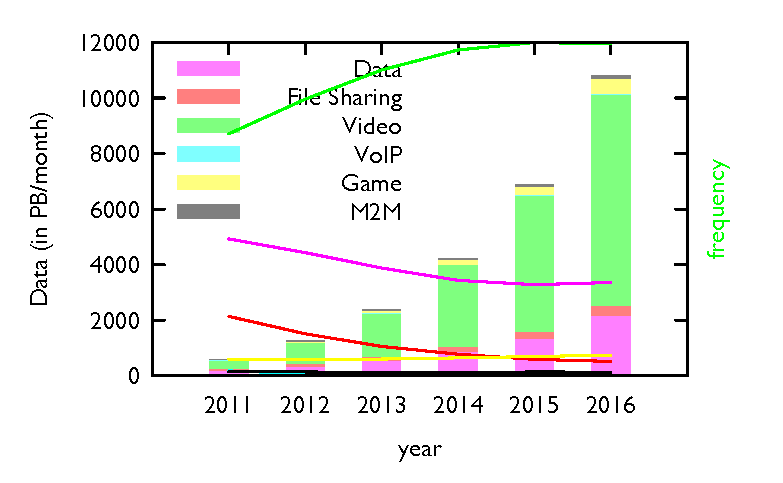
\includegraphics[width=0.45\textwidth]{mobile}
    \label{fig:internet}
}
\subfigure[global Internet traffic trend]{
    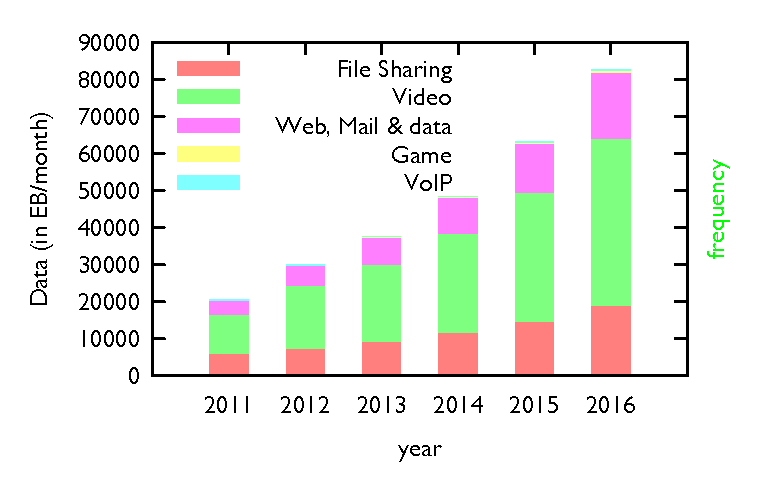
\includegraphics[width=0.45\textwidth]{internet}
    \label{fig:mobile}
}
\caption{Cisco Visual Network Index reports on global network
  traffic per application. Subfigure~\ref{fig:internet} provides details on the global Internet
  traffic trends, while Subfigure~\ref{fig:mobile} focuses on Mobile Internet
  traffic.}
\label{fig:internet_applications}
\end{figure}


\begin{table}
\begin{center}
\begin{tabular}{ | l | c c c c | }
  \hline
  Application  & rate & latency & jitter  & \# connections \\
  \hline
  web          & 0    & 0       & 0      & 0\\
  video        & 0    & 0       & 0      & 0\\
  p2p          & 0    & 0       & 0      & 0\\
  voip         & 0    & 0       & 0      & 0\\
  game         & 0    & 0       & 0      & 0\\
  \hline
\end{tabular}
\end{center}
\caption{Network performance requirement for a set of popular traffic classes.}
\label{tbl:application_requirement}
\end{table}



% a historical prespective on computer networks 
One of the ideas that formed the subjective condition of the digital revolution
of our era, was the concept of computer networking. The initial goal of this
concept was to develop a new communication architecture that would allow
continuous communication over a redundant network, even when a significant
number of vertex was destroyed.  The main building block of computer networks is
the idea of packet-switched networks~\cite{Licklider1963}.  This idea gave birth
to the pioneer of today's Internet, the {\it ARPANET}~\cite{Mills:1987tt},
allowing for the first time in computing history communication between multiple
computers over a mess network. The initial set of applications
that were standardised where : e-mail~\cite{RFC0561},
ftp~\cite{RFC0354} and voice~\cite{RFC0741}. This initial implementation was
later replaced by the NSFNET in the 80's, which finally devolved in today's
Internet. Additionally, the first transition to the NSFNET gave birth to the 
currently default protocol suite of TCP/IP~\cite{Clark:1988}, which has
seen minimum changes on its semantics and format since then.

% why computer networking is successful from the user perspective
Since the time of the ARPANET, computer networks have seen a significant
elevation on their role in the social apparatus of our world due to a number of
reasons. One of the most important trends, that boost their role, was the radical
reduction in cost, size and capabilities of network-enabled personal
computers, following Moore's Law model. In addition, the programmable nature of
the computer CPU, makes it an elegant platform to develop applications that
introduce seamlessly new functionalities. Nowadays, programmable CPUs are
integrated in a number of multipurpose devices, like mobile phones, display
devices etc, while personal computers, with their ability to transform in size,
introduce new personal computers concepts, such as laptops, tablets and other.
As a result, the paradigm of one computer per household of the 90's rapidly
shifted to the paradigm of multiple devices per user, replacing
a number of everyday single-purpose devices~\cite{Dholakia:2006vn}.  On one hand, this
augmentation in computational devices requires new modes of communication that
allow devices to share consistently state, driving a significant development in
computer network technologies. A number of network-enabled applications are
developed to address these requirements, while new network concepts are
introduced like home networks and hotspots. On the other hand, the elevated role
of computer networks and the introduction of the cloud computing paradigm,
introduce a number of internet-wide services with a global scope. These new
applications introduce a number of new assumptions on performance and connectivity
over the Internet abstraction. 

% why computer become important for the global economy too? 
In parallel with the development of the personal computer paradigm, computer
network are widely adopted as an integral asset for industry.
Currently the Internet produces 4,3\% of the global GDP. Computer Networking
and the Internet, provide the middleware to interconnect modern multinational
businesses. In the business domain computer network have become popular and
important for two main reasons: computer networks provide a cheap and fast
medium communication medium to interconnect the business logic, and the provide
a global medium to provide content to users. The adaptation of computer network
has further augmented through the utilisation of the cloud as a medium to
offload infrastructures to 3rd party cloud providers, reducing to a great extend
the cost of running services in house.\todo{add a reference to the value of the
cloud industry.} 

% How computer application mix looks in the wire? 
This wide adaptation of computer networks has introduce a number of new use cases and
applications for computer networks. Such applications introduce new assumptions over the
network abstraction. Further the popularity of network applications has a high churn over
the years, making longterm resource allocation through networking planning difficult.  In order to exhibit this trend,
we plot in Figure~\ref{fig:internet_apllications} the global prediction on traffic volumes
per applications for five years. We use data from cisco visualization index white
papers~\cite{Mobile:2012vd,Cisco:2012wu}. In histogram we can see that network traffic is
expected to increase an order of magnitude for the mobile environment, while the global
Internet traffic is expected to increase four times. In parallel, this volume increase is
uneven between traffic classes. File sharing services are expected to reduce their share
of the total volume, replaced by web and video delivery services. 

% what about the application requirements 
The problem of resource allocation is further augmented by the diverse nature of network
applications. In order to describe better the impact of these traffic changes, we list in
Table~\ref{tbl:application_requirement}, some key properties and requirements for each
traffic class. We can see in the list that applications in general have pretty diverse
properties and their requirements are difficult to fulfil during congestion. 

% How does the network look like on the edge. 
High diversity is also observed on the connection medium of the computer
networks. Currently, ethernet is currently the predominant link layer protocol
in the Internet. This dominance didn't occur since the beginning of computer
network. The main philosophy of the OSI protocol, and in respect of the TCP/IP
protocol, was the bstraction of the link layer details in order to hide the
running war between the different technologies (ATM, Token Ring). In the 80's
the low cost difference of Ethernet establish it as the leader of the market
ever since. As a result, this monoculture in the link layer, lead to the
standarization of the protocol as the de-facto link layer protocol. Since then,
although the Ethernet abstraction is global, the link layer technologies are
diverse, Introducing a number of different mediums in the Ethernet abstraction.
Currently Ethernet is exposed over coper and optical links, as well as
off-licence radio frequencies and mobile networks. Although the Ethernet
abstraction is persistent among all these mediums, the properties of the link
are diverse and difficult to keep the performance abstraction consistent.

In respect, the Internet is a highly heterogeneous 


\subsubsection{Computer network ossification}

% how does computer networks look like, How the Internet looks like?

% Introduce the reason behind protocol ossification and computer network
% evolution limitations 

% Some concrete examples of how computer networks are insufficient 

Further, the connectivity costs have reduced to a great extend, allowing
intermittent user connectivity.  Additionally, Internet since its first days,
through its simple network abstraction and it ability to self-configure and
self-heal, provides an excellent medium to interconnect heterogenious devices
and provide the connecting medium for a number of services. A connecting entity
is solely required to implement a TCP/IP stack and peer with a forwarding
entity, in order to reach any exposed Internet service.  Because of these
properties, there is a long discussion in govermental level to proclaim Internet
connectivity as a fundamental human right~\cite{klang2005human}.

% What are the communcation pattern of modern Internet?  

% How the communcation medium has changed? 

% wrap-up - Things are tricky. 

Currently, the set of Internet-wide services over the Internet in the last
decade increased exponentially. This increase in internet use cases introduced
in the network a number of new performance requirements which made traditional
network resource allocation mechanisms and network planning innefective.

In computer network literature a number of clean slate architectures has been
introduced that can address the hard problem of resource allocation, through the
design of new protocols. 
The type of the provided is diverse and thus they require
from the network diverse properties. 

\todo{Add a case for Amdahl's law.}

\section{Contributions}
\label{sec:intro:contributions}

\section{Outline}
\label{sec:intro:outline}

\section{Publications}
\label{sec:intro:pubs}

%%% Local Variables: 
%%% mode: latex
%%% TeX-master: "../thesis"
%%% End: 

\chapter{Background} \label{ch:background}

This chapter provides an extensive discussion on network control in
packet-switched networks.  We motivate the discussion on network control,
describing the architecture of network devices and their inherent physical
limitations (Section~\ref{sec:background:forwarding}) and elaborate on existing
network control mechanisms for production networks
(Section~\ref{sec:background:netcontrol}).  Furthermore, we present three
significant efforts in flexible network control, namely Active Network,
Devolved Control of ATM Networks (DCAN) and Software Defined Networking (SDN),
proposed by the research community to address limitations in network control
schemes (Section~\ref{sec:background:netcontrol}). Finally, we focus on the SDN
paradigm and present some of its applications in a series of current network
problems (Section~\ref{sec:background:ofapp}).

\section{Forwarding Devices and Control} \label{sec:background:forwarding}

This section focuses on Ethernet networks and provides a high-level design
overview of a common forwarding device, the \emph{switch}. Using this model we
highlight the physical limits of network performance in the control and data
plane and motivate our discussion on control effectiveness.

\begin{figure}
  \centering
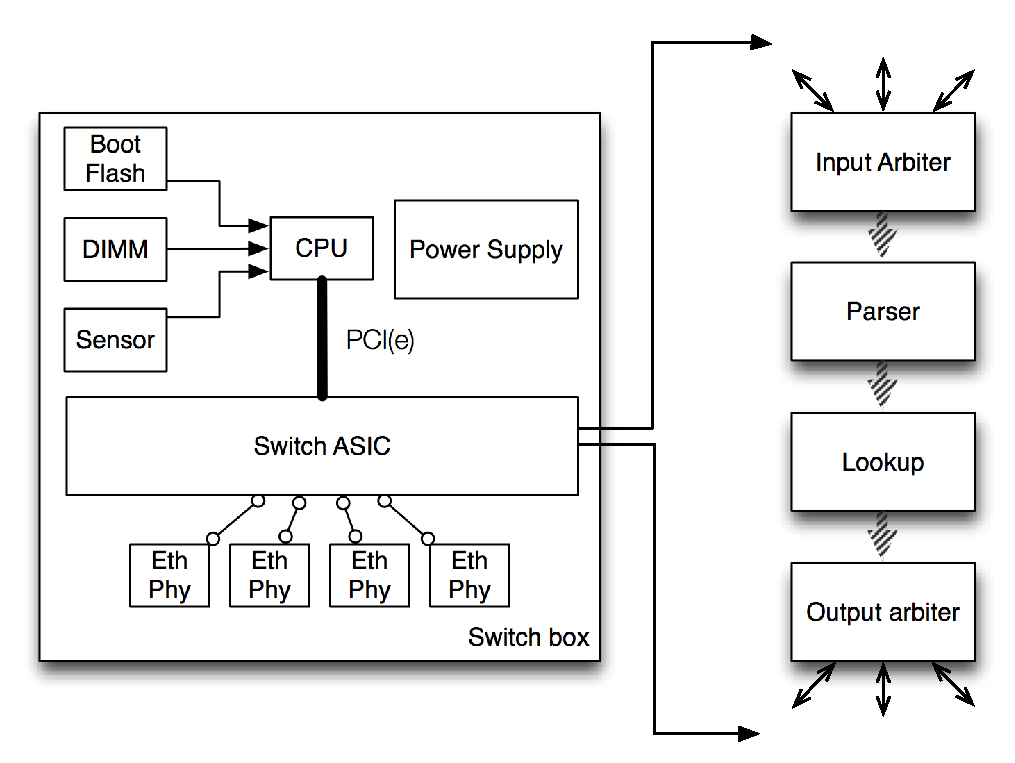
\includegraphics[width=0.6\textwidth]{Background/BackgroundFigs/switch_design}
\caption{Generic design model of hardware switches.}
\label{fig:background:switch_design}
\end{figure}

Ethernet switches multiplex Ethernet broadcast domains and provide
collision-free connectivity between network segments.  Network vendors provide
a wide range of switch types with variable functional capabilities (e.g. VLAN
support, multilayer switches).  For example, an unmanaged switch provides
elementary non-configurable functionality with low 1 GbE port density, while a
distribution switch provides high 10 or 40 GbE port density and a range of
traffic management applications.  We use the Top-of-Rack~(ToR) switch type to
elaborate on the architecture of modern hardware switches.  ToR switches are
used in datacenter and enterprise networks to multiplex traffic between
the edge and distribution network layers. Forwarding functionality is
implemented  using Application-Specific Integrated Circuit~(ASIC) silicons,
providing multi-GbE line-rate non-blocking traffic forwarding.
Figure~\ref{fig:background:switch_design} presents a model for ToR switch architectures
which consists of the following components:

\begin{itemize}
  \item \emph{Co-processor/Management CPU}: Switch devices use a programmable
      CPU to fulfil control plane computation requirements. The CPU hosts a
      minimal operating system, responsible for translating the device
      configuration into appropriate ASIC manipulations at run-time. Vendors
      usually employ low-power CPUs, like SoC PowerPC and ARM processors. The
      CPU is equipped with runtime (Boot Flash and RAM) and persistent (e.g.~SD
      cards) memory modules. In general, switch CPUs provide sufficient
      computation resources to run the switch control-plane functionality, but
      they cannot accommodate intensive processing tasks. The switch OS usually
      provides elementary remote control services, like telnet and SSH, command
      line/web interfaces and SNMP access to the switch state. 
 
  \item \emph{Switch ASIC}: The switch
      ASIC~\mycite{hp-asic,broadcom-asic,intel-asic} implements in hardware the
      data plane functionality. The capabilities of an ASIC are variable,
      depending on the vendor and the cost, and define the data plane
      performance limits of the device.  ASICs have an expensive development
      cycle, consisting of long design and testing periods, and require
      significant human labour and material resources requirements. As a result,
      ASIC innovation has a high latency before reaching production, while the design
      details remain undisclosed.  

    The ASIC packet processing pipeline commonly consists of four stages.  The
    \emph{input arbiter} stage multiplexes and synchronizes packets from the
    Ethernet ports to the main processing pipeline of the silicon. The arbiter
    ensures non pre-emptive packet processing, by bridging the mismatch between
    the silicon processing clock rate and the link rate. The pipeline also
    contains a \emph{protocol parsing} stage and a \emph{memory lookup} stage.
    The protocol parser extracts significant packet fields from network
    packets, used by the memory lookup module to define packet processing and
    forwarding.  The lookup stage uses a memory module, integrated or external
    to the ASIC, which contains the forwarding policy.  Memory modules exhibit 
    trade-offs between cost and access speed and  memory cost and memory
    management complexity\footnote{A 32-bit TCAM lookup pcore running on a
        Virtex-5 FPGA~\mycite{virtex5} with 550 MHz clock rate requires 1 clock
        cycle for a lookup, translating into a 2 ns delay. A DDR3-2400 SDRAM
        memory module operating at 1200 MHz and requiring 9 clock cycles per
        data access has a 9 ns lookup latency, while a PC133 SDRAM operating at
        133 MHz and requiring 3 clock cycles per data access has a 20 ns
    lookup latency.}. Finally, the \emph{output arbiter} module is responsible for
    applying modifications to the packet and forwarding it to the appropriate
    output queue. The processing pipeline may contain additional modules which
    extend functionality, providing access control list (ACL), virtual network
    queues, and flow statistics monitoring.

  \item \emph{ASIC-CPU interconnection}: The management CPU is connected to the ASIC
    over a PCI or PCI-express channel. The interconnection provides an
    elementary bi-directional channel allowing the CPU to program the ASIC
    through its register API, and the ASIC to propagate exceptional packets to
    the CPU\@. The channel provides sufficient bandwidth for basic control plane
    communication, but it is not designed to handle high rate information. For
    example, current Broadcom Trident chipsets use a PCIe 4x or 8x bus,
    achieving 2 to 4 Gbps capacity.  

  \item \emph{Memory}: Apart from in-ASIC memory modules, switches
    also use multiple memory types to support the run-time requirements of the
    firmware. A switch is usually equipped with CPU Boot Flash, to boot the
    OS/firmware, DIMM RAM and multiple memory slots, for control plane logging
    and configuration persistence.

  \item \emph{Ethernet ports}: The receipt and transmission of Ethernet packets
    is implemented by a separate hardware module, 
    implementing the physical and MAC layers of the protocol. The port module 
    connects with the  ASIC through a Media Independent Interface (MII) and
    contains small packet buffers to reduce packet loss.  
\end{itemize}

In terms of data plane performance,  the forwarding capabilities of an ASIC are
upper-bound by the transistor density and size, as in general purpose CPU
silicones. A ToR switch uses a single ASIC, supporting up to 100 Gbps of processing
capacity.  In terms of control plane performance, the primary limitations are the
capacity of the communication bus between the coprocessor and the ASIC, the
design of the interface between the two entities, and the processing capabilities
of the switch CPU\@.  For a ToR switch, the vendors usually provide a PCIe
communication bus, supporting capacities on the order of a few Gbps, while
CPUs have limited processing capabilities (Section~\ref{sec:oflops-switches} provides details
on some off-the-self ToR switches).

ToR switches are simple switch devices and provide low to medium forwarding
capacity. Vendors provide network devices that support higher link capacities
and enhanced functionalities that have more complex architectures.
Multi-chassis switches and routers, used in the core of large networks, cannot
fit their processing pipeline requirements in a single ASIC\@.  Packet
processing is distributed between multiple silicons, interconnected using
complex CLOS crossbar fabrics with non-blocking Terabit backplane
capacities~\mycite{juniper_t_series}. Network control in such devices exhibits
similar high complexity, and uses distributed forwarding tables and cache
coherent protocols to ensure state consistency~\mycite{cisco_cef}. In such
devices, ASIC control is complex, inflexible and slow.  

\section{Forwarding Control in Production Networks} \label{sec:background:netcontrol}

Current network architectures and technologies set dynamic control as a
fundamental design goal.  Existing standardized approaches provide
\textit{distributed}, \textit{autonomous} and \textit{resilient} control,
influenced extensively by the end-to-end Internet principle. The administrator
is responsible for defining the local policy of a device, and at run-time
distributed protocols reconstruct the global network state.  Using the global
network state, the forwarding logic determines an optimal forwarding policy
which optimizes specific aspects of network performance.  For the rest of this
section we present the control plane functionality in the data-link and network
layers of the network stack. 
% existing production-level protocols that enable distributed network control. We
% focus on the Data-Link and Network layer protocols as these layer define the
% hop-by-hop forwarding policy.

\subsection{Data-Link Layer Control}

Data-link layer control protocols provide loop-detection, VLAN and QoS
configuration automation. Loop detection is used to avoid packet loops in
networks with redundant connectivity, as Ethernet specification doesn't
support packet timeout functionality.  The Spanning Tree Protocol~(STP) was a
first attempt to address this problem, standardised by IEEE in
802.1D-1998~\mycite{ieee_802_1d_1998}. The protocol implements the distributed
spanning tree construction algorithm, presented in~\mycite{Perlman1985}. The
algorithm uses broadcast messages to discover a spanning tree over the network
graph, with respect to a common root switch. For each port, the switch maintains
a state machine, which disables packet forwarding when the respective link is
not part of the spanning tree.  Because the initial definition of the protocol
faced significant convergence delay after a network change, IEEE introduced the
Rapid Spanning Tree Protocol~(RSTP), an evolved version of
STP~\mycite{ieee_802_1d_2004}.  In addition,  IEEE Multiple Spanning Tree
Protocol~(MSTP)~\mycite{ieee_802_1q} developed a modified version of the protocol,
optimized for VLAN-based networks. MSTP constructs a spanning tree for each
VLAN, which effectively  reduces unnecessary port blocking. Cisco has developed a
series of proprietary protocols to address the problem in a similar
manner~\mycite{pvst,pvst+}.  Finally, IEEE recently defined an STP protocol to
detect and use redundant paths in the IEEE 802.1aq standard~\mycite{ieee_802_1aq}.

In terms of configuration automation, network vendors and standardization bodies
have developed a number of protocols to disseminate device status between
neighbouring nodes. This functionality differs significantly between vendors.
In this class of protocols we consider Link Layer Discovery Protocol
(LLDP)~\mycite{ieee_802_1ab}, Cisco Discovery Protocol
(CDP)~\mycite{cdp},  Extreme Discovery Protocol~(EDP) and Nortel Discovery
Protocol~(NDP). Finally Cisco has developed the VLAN Trunking Protocol (VTP), a
protocol which reduces the VLAN configuration burden in inter-switch trunk
links.

In the class of data-link layer protocols, we also consider the MPLS
protocol~\mycite{RFC3031}.  MPLS is a circuit-based technology and uses labels
to forward packets, effectively reducing forwarding table sizes.  MPLS circuit
creation is automated through the Label Distribution Protocol
(LDP)~\mycite{RFC5036}, which uses an underlying routing protocol to compute
and setup labels across the network. The IETF defines an RSVP resource
allocation mechanism over MPLS~\mycite{RFC3209} and
\textit{Autobandwidth}~\mycite{osborne02}, an automatic mechanism to enforce
such resource allocation.  Because MPLS does not support resource policing,
autobandwidth monitors the bandwidth requirements for each circuit and
reconfigures circuits in order to fulfil measured requirements.
\mycitet{Pathak2011} analyse an autobandwidth deployment on the MSN network and
highlight significant latency effects as a result of the autobandwidth
functionality.

% In Data-Link layer we can also consider the MPLS protocol 

\subsection{Network Layer Control}

Control in the network layer is responsible for collectively constructing an optimal
forwarding table between the routers of a network.  Routing protocols are generally
categorized into three classes: \emph{Link State}; \emph{Distance Vector}; and
\emph{Path Vector}. Link state protocols theory build on-top of the Djikstra
algorithm~\mycite{Djikstra1959}. Routers disseminate their local forwarding
configuration to the rest of the network.  Using this global state exchange,
each router is able to construct the global connection graph. Each router can
use the graph to calculate the minimum spanning tree of the network, using
Djikstra's algorithm.  Currently there is a plethora of Link State protocol
specification in the network community.  IETF has developed the OSPF
protocol~\mycite{RFC2328}, an IPv4 specific routing protocol, while the Open
Systems Interconnection~(OSI) organisation has defined the IS-IS
protocol~\mycite{RFC1142}, a network layer agnostic routing protocol.  Link
State routing protocols provide high flexibility in defining the optimisation
function of the routing system.  Each router has a view over the complete graph of
the network, and routers can propagate multiple link performance indexes
(e.g.~link load, link speed ).  Nonetheless, the optimization function must be
homogeneous across the network, in order to avoid routing loops.

Distance Vector protocols follow a different routing approach, based on
Belman-Ford~\mycite{bellman1956}. The routing table is constructed using
information from adjacent routers. Network changes are slowly propagated across
the network, through point-to-point information exchanges, until all routers
converge.  IETF developed the RIP  protocol~\mycite{RFC2453} to implement Distance
Vector routing, while Cisco has developed the proprietary IGMP
protocol~\mycite{Rutgers1991}. Distance Vector protocols are less extensible in
comparison to Link State protocols, but exhibit lower computational and memory
requirements.

Finally, Path Vector protocols evolve Distance Vector protocols to support
inter-domain routing. Path Vector routing discloses minimal information in
terms of the forwarding policy of an Autonomous System (AS), advertising only
supported network paths, As a result, Path Vector protocols do not define a
routing algorithm.  The BGP protocol~\mycite{RFC1265} is currently the
predominant Path Vector routing implementation.  As Internet increases in size,
BGP deployment has experienced significant scalability problems and motivated
some of the network control frameworks presented in
Section~\ref{sec:background:netcontrol}.  A significant scalability problem in
BGP is the impact of path updates in the functionality of routers in large
ASes. Path updates are handed by the iBGP protocol using a full-mess
dissemination approach, which incurs significant router load and memory usage.
A widely used approach in addressing this problem uses Route Reflectors
(RR)~\mycite{RFC4456} hosts, which form a hierarchical update dissemination
mechanism and reduce forwarding information on each router. A further
improvement on iBGP scalability was developed by~\mycitet{Caesar2005} as part of
the Routing Control Platform~(RCP), proposing control centralisation similar to
the SDN paradigm. RCP basically proposed the centralisation of the BGP routing
table calculation within an AS.

Due to their distributed nature, routing protocols provide long-term routing
resilience, while their mathematical foundations are provably correct.
Nonetheless, the control abstraction of these protocols is not a good fit for
an administrator to exercise dynamic control over the network. For example, the
ability of a network manager to estimate the impact of a significant forwarding
policy update is reduced as the network size increases.  In 2008, the global
Internet was severely affected by a BGP misconfiguration in the Pakistani
national ISP in an effort to control traffic from the YouTube
service~\mycite{bgp_config_error}.  In addition, routing inconsistencies during
routing changes can significantly impact network performance.
\mycitet{Watson2003} evaluate that OSPF functionality in a regional ISP exhibits
high routing churn, even during periods with low control plane activity, while
the latency in convergence after a network change is, on average, on the order of
seconds. Similar results have been observed in BGP\@.  \mycitet{Kushman2007}
highlight a strong correlation of BGP instability and VoIP
performance. Modern high speed networks require higher flexibility and
responsiveness in the control abstraction. 

\section{Programmable Network Control} \label{sec:background:prog_control}

The limitations of current standardized network control frameworks have
motivated the research community to reconsider their design.  The rest of this
section presents three significant efforts, namely Active Network, Devolved
Control of ATM Networks (DCAN) and Software Defined Networking (SDN). 

\subsection{Active Network}

The network research community has highlighted the ``inevolvability'' of network
functionality, often termed \textit{protocol ossification}, since the early
90's.  \mycitet{OMalley1992} challenged the generality of the OSI network model
and suggested synthesizable protocol parsers, which can incorporate variable
numbers of layers in forwarding devices.  Motivated by these observations, DARPA
funded the \emph{Active Network} project~\mycite{darpa_active_net} to develop
next generation network devices supporting seamless network upgradability. 

Active Networks evolve the packet processing pipeline. Specifically, they
introduce the notion of \emph{capsules};  network packets carrying data and
processing code. On each hop, the default packet processing logic is extended
with the capsule code. Active Networks provide user-driven protocol upgrades
without any device or driver modification.  
% In addition, the development of novel
% programming languages, like Java, provided the building blocks to implement code
% distribution frameworks.

Active Network research defined two primary design aspects:
the {\bf capsule API and format} and the {\bf switch architecture}. In
terms of capsule format, the Active Network community defined the Active Network
Encapsulation Protocol~(ANEP)~\mycite{alexander1997a}, adopted by the ANTS and
Sprocket capsule programming frameworks.  Sprocket~\mycite{Schwartz2000} was
developed by BBN technologies and defined a capsule programming language, based
on C. Sprocket removed all insecure C structures, like pointers,
and provided native support for SNMP browsing.  Its compiler produced MIPS
assembly code and the capsule code was executed using a MIPS VM on each networks
device.  Sprocket did not persist any state on the switch, but allowed
capsule code to modify packet data.  ANTS~\mycite{Wetherall1998} was an attempt
by the MIT Active Network group to develop a JAVA-based capsule programming
environment.  ANTS used a restricted version of the Java language, and switch and
capsule integration was defined using Java interfaces. Capsule code could
persist state on switches and modify packet content. An interesting
functionality of the ANTS framework was the code dissemination mechanism. An
end-node would deploy its protocol functionality solely to the local Internet
gateway, and the code would be forwarded along the network towards the
destination, hop-by-hop. Finally, the University of Pennsylvania's Active Network
group developed PLAN~\mycite{Hicks1998}, an OCaml-based approach to capsule
programming.  PLAN did not follow the ANEP packet format. A PLAN capsule
contained code and data, with the capsule code replacing the network header
information. In order to secure switch infrastructure, the language disallowed
packet data modification or switch state persistence.  Ultimately, the language
provided a framework for programmable control plane.

In terms of Active Network platform architecture, the community developed a
number of architectures, addressing many efficiency aspects in capsule
processing. The University of Pennsylvania developed the SwitchWare Execution
Environment (EE)~\mycite{Alexander1998}.  The architecture developed an OCaml
capsule processing framework providing enhanced security for the switch and
capsule execution environment.  SwitchWare used SANE~\mycite{Alexander1998b}, a
trustworthy operating system, to secure the functionality of the switch, and
build on top of its primitives to provide higher level of security. The platform
addressed issues regarding secure execution and authentication as well as
capsule code verification.  PLANet~\mycite{Hicks1999} and Active
Bridge~\mycite{Alexander1997b} used the SwitchWare framework to implement novel
functionality in Active Network. 

The Active Network group in the University of Arizona presented a switch
architecture which optimized multi-layer packet processing using the
communication-oriented Scout OS~\mycite{Montz1995}. On top of Scout, the group
developed the Liquid Software API~\mycite{Hartman1999}, providing a tight
integration between the OS and the JVM, and improved capsule processing using
the JIT JAVA compiler. 

The CANEs project~\mycite{Chae2002} from the Georgia Tech Active Network group
proposed a switch architecture, which improved flexibility in multi-protocol
packet processing. Specifically, it defined a number of abstractions, which
allowed multiple protocol stacking on the forwarding path. CANEs project build
on top of the Bowman Switch OS~\mycite{merugu1999} and established a simple and
efficient abstraction over switch resources.  Researchers from Columbia
University developed the NetScript switch programming
language~\mycite{daSilva2001}, designed for flexible protocol processing
definition and composition. The language provided seamless extensibility in
protocol implementation logic, providing three types of protocol composition:
layered composition; composition through protocol bridging; and end-to-end
composition.

Finally, a joint effort between ETH and the University of St. Louis, developed a
high performance capsule-enabled switch design. The High Performance Active
Network Node (ANN) switch architecture~\mycite{Decasper1999} used an FPGA-based
CPU on each ATM interface to handle capsule execution.  The CPU could run the
ANTS EE and provided an IPv4 and IPv6 protocol processor supporting Gigabit rates. 

Active Networks addressed a number of interesting problems in control plane
functionality, especially issues like controllability and evolvability, and
motivated recent efforts in the field.  Nonetheless, proposed architectures
followed a complex and clean-slate approach, and thus reduced their applicability
in production environments. In addition, Active Network functionality
benefited highly from the relatively low link rates of the time, which were manageable
by the CPU chipsets. The exponential increase in link capacities, supporting up
to Gigabit rates, restricts our ability to support the rich programmability of
Active Network.  Finally, the flexibility provided by Active Networks raised
significant concerns on network security and resource controllability.  

\subsection{Devolved Control of ATM Networks}

\begin{figure}
  \begin{center}
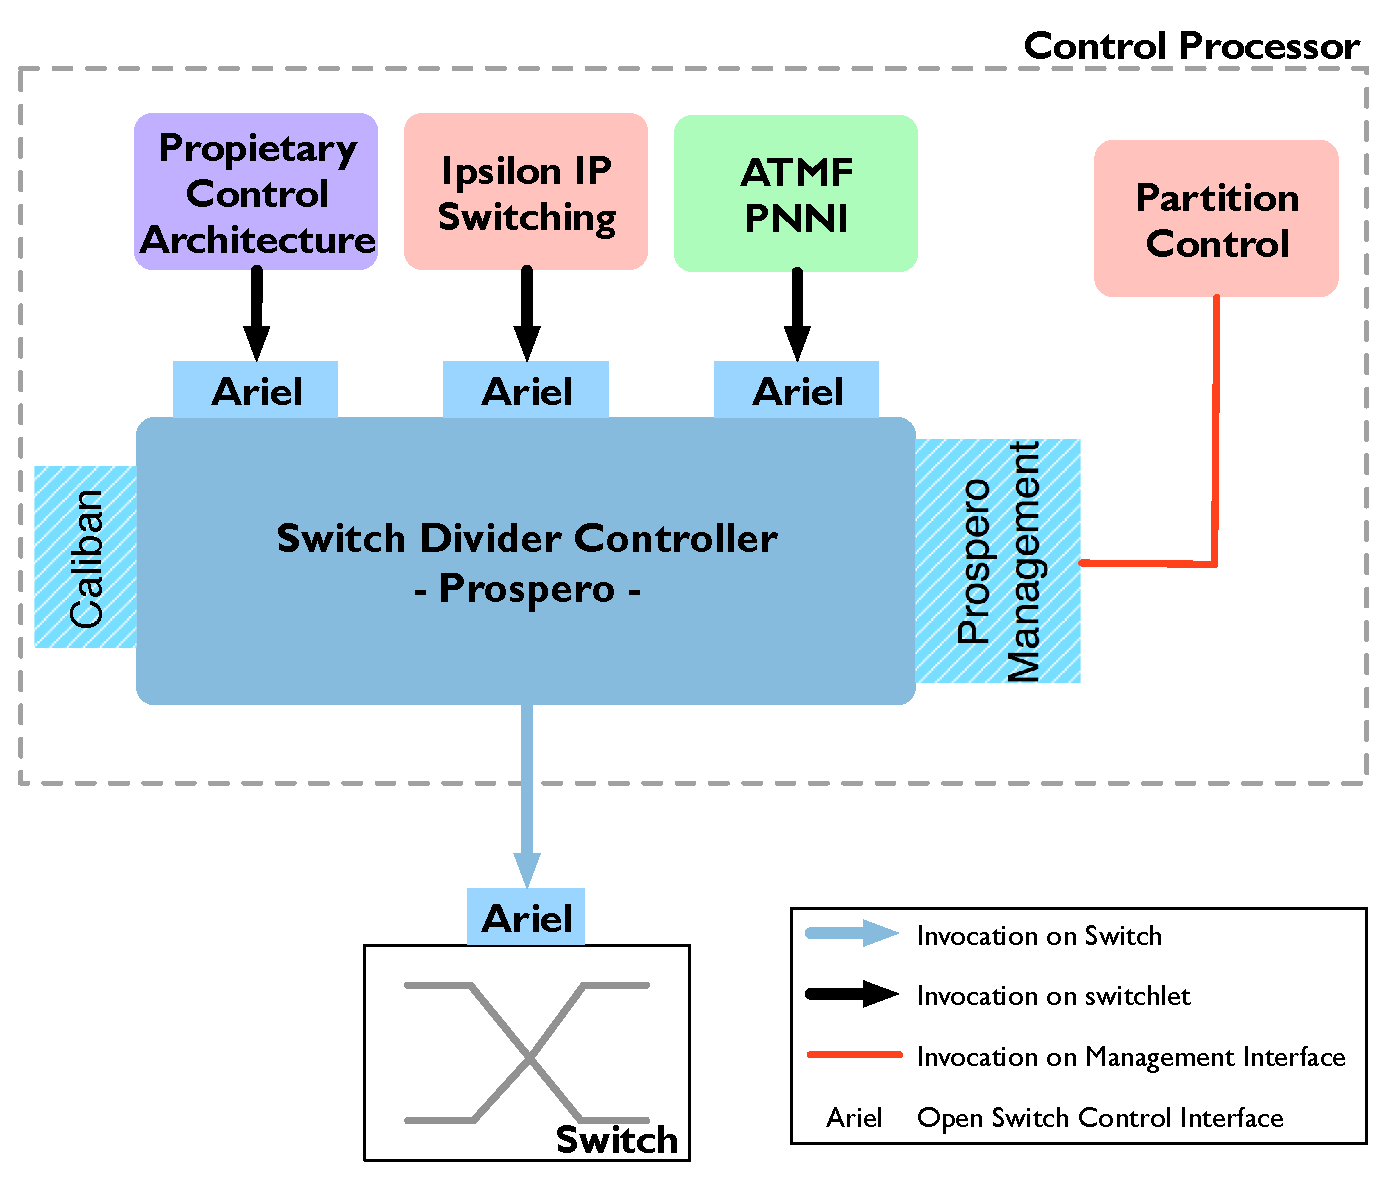
\includegraphics[width=0.7\textwidth]{Background/BackgroundFigs/tempest_arch}
\caption{Tempest switch architecture~\mycite{Merwe98}.}
\label{fig:background:tempest_arch}
\end{center}
\end{figure}

Active Networks focused extensively on Ethernet technologies and strived to
develop protocol evolvability. A similar approach was developed in the
University of Cambridge for the DCAN~\mycite{dcan} project, focusing
primarily on control evolvability and network virtualisation in ATM networks.
DCAN tried primarily to simplify the control plane of ATM devices, in order to
support network multi-functionality. Similar efforts were developed by IETF
through the General Switch Management Protocol (GSMP)~\mycite{RFC3292}.

\mycitet{Rooney1998} presented Tempest, a novel ATM switch architecture, which
enabled clean separation of the control and forwarding plane of an ATM
switch. Similar to the SDN approach,  the control plane was centralised in a
single programmable entity, which could implement intelligent and dynamic
forwarding.  The implementation of Tempest was logically divided between three
subsystems, depicted in Figure~\ref{fig:background:tempest_arch}. The figure
presents how a single switch is able to function in parallel as an IP router, an
ATM switch and a Hollowman controller~\mycite{Rooney1997}, a devolved ATM
control framework. 

\paragraph{Prospero Switch Divider} 

The \emph{Prospero} abstraction provides a mechanism for virtualising ATM switch
resources into multiple virtual switches, called \emph{switchlets}, through a
resource control interface.  A switchlet controls a subset of switch ports,
VCI and VPI mappings, packet buffers and bandwidth. Prospero used the ATM QoS
principles to implement packet buffer and bandwidth virtualisation.
Fundamentally, Prospero is responsible for mapping the control interface, exposed to
controllers, to the underlying switch functionality. 

\paragraph{Ariel Switch Independent Control Interface} 

Switchlets exposed forwarding control through the Ariel Interface. The Ariel
Interface organises network control through six control objects:
\emph{Configuration}, \emph{Port}, \emph{Context}, {\it Connections},
\emph{Statistics} and \emph{Alarms}.  The Configuration object provides details
for the switch configuration; the Port object provides primitive controllability
of ports (e.g.~state, loopback functionality); the Context object enables QoS
policy control; the Connection object exposes control of VPI/VCI mappings; the
Statistics object exposes packet and byte counters; and the Alarms object pushes
state change notifications to the controller. Tempest switches executes an Ariel
server and translates Ariel requests to Prospero control requests. Ariel
was fundamentally an abstraction layer between the switch silicon and the
Prospero control interface. 

\paragraph{Caliban Switch Management Interface}

In addition to network control, Tempest also supports evolved network
management through the Caliban interface. The interface functionality is
similar to the SNMP protocol. Caliban provides fine level SNMP-style
information, as well as higher level aggregation operations over the switch
state. 

In addition to the redefinition of the network control abstraction, Tempest also
proposed a relaxed network resource management scheme.  Specifically, the
architecture proposed a measurement-based admission control mechanism for
circuit establishment~\mycite{Lewis1998}. The measurement scheme redefined the
static resource allocation scheme in an ATM network, and used effective bandwidth
measurement techniques to estimate available resources and provide higher
utilisation of network resources, with minimum relaxation of the QoS guarantees. 

Tempest defined a highly efficient network control abstraction, which motivated
modern network control approaches, like the SDN, to reimplement it over Ethernet
devices.  The simplicity of the control abstraction permitted
integration of the technology with existing forwarding devices, and enabled line
rate forwarding and efficient resource control.  Nonetheless, its strong
reliance on the ATM technology made the approach less relevant for the modern
Ethernet-dominated networks~\mycite{Crosby2002}. 

\subsection{Software Defined Networking}\label{sec:background:sdn} 

SDN~\mycite{sdn}, the most recent network control paradigm, provides a pragmatic
approach to control evolvability. SDN employs  a clean separation between the
control and forwarding plane of a network device. The control logic is
removed from the network device and implemented by a separate service.  A well
defined protocol establishes the integration between the two entities. 

The SDN paradigm is motivated by relevant earlier attempts in network
programmability(Active Network and DCAN), but follows an evolutionary approach.
The paradigm is motivated by two key observations.  Firstly, the evolution of
computer networks has collapsed the layers of the OSI and TCP/IP models.
Production networks use network devices (e.g.~firewall, NAT, layer-5 switches)
which operate on multiple layers of the network and engage extensively in layer
violation.  The SDN paradigm provides a unifying cross-layer control model which
fits such functionality under a single interface.  Secondly, although network
complexity has increased, network devices still expose stand-alone,
decentralised and inflexible configuration mechanisms (e.g.~remote logic, CLI
interfaces), and employ proprietary control protocols, which reduce device
interoperability within the network. The SDN architecture establishes
centralised and unified management, supporting reactive control.  The \of
protocol is currently the pre-dominant implementation of the SDN paradigm.

\subsubsection*{\of Protocol} 

\begin{figure}
  \begin{center}
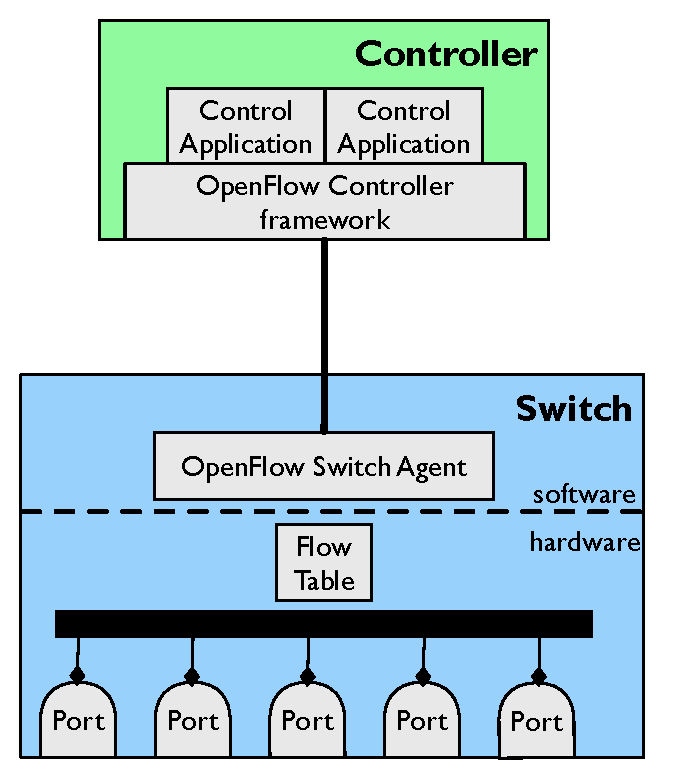
\includegraphics[width=0.40\textwidth]{Background/BackgroundFigs/openflow-schema}
\caption[An elementary \of setup]{An elementary \of setup, consisting of a
switch and a controller.  implementating \of has motivated the definition of
additional abstractions for control application and silicon adaption 
agents.}
\label{fig:background:openflow-schema}
\end{center}
\end{figure}
\begin{table}
\begin{minipage} []{0.99\textwidth} 
    \begin{tabular}{|p{4cm}  | p{2cm} |p{0.1cm}|p{4cm}  | p{2cm} |} 
      \hline
      Field & \of Version & & Field & OpenFlow Version \\ 
      \hline
      Src \& Dst MAC addr. & 1.0~\footnote{Since version 1.1 the protocol
        permits masked mac address matching} & & input port & 1.0 \\ \hline
      VLAN ID & 1.0 & &VLAN PCP & 1.0 \\ \hline
      IPv4 src/dst addr. & 1.0 & & IPv4 ToS & 1.0 \\ \hline
      ICMPv4 Type \& Code & 1.0 & & TCP/UDP/SCTP src/dst port & 1.0 \\ \hline
      MPLS label & 1.1 & & Metadata & 1.1 \\ \hline
      MPLS class & 1.1 & & IPv6 src/dst addr. & 1.2 \\ \hline 
      IPv4 proto & 1.0 & & IPv6 flow label & 1.2 \\ \hline
      ARP opcode & 1.0 & & ICMPv6 type \& code & 1.2 \\ \hline 
      ARP src/dst IPv4 address & 1.0 & & ICMPv6 Network Discovery target address & 1.2 \\ \hline 
      ARP src/dst MAC address & 1.2 & & ICMPv6 Network Discovery src/dst MAC address & 1.2 \\ \hline 
    \end{tabular}
%%  \end{minipage}
%%  \begin{minipage} []{0.49\textwidth} 
%%    \begin{tabular}{} 
%%      \hline
%%      Field & OpenFlow Version \\  \hline
%%      IPv4 ToS & 1.0 \\ \hline 
%%      ICMPv4 Type \& Code & 1.0 \\ \hline
%%      TCP/UDP/SCTP src/dst port & 1.0 \\ \hline
%%      Metadata & 1.1 \\ \hline
%%      IPv6 src/dst addr. & 1.2 \\ \hline
%%      IPv6 flow label & 1.2 \\ \hline
%%      ICMPv6 type \& code & 1.2 \\ \hline
%%      ICMPv6 Network Discovery target address & 1.2 \\ \hline
%%      ICMPv6 Network Discovery src/dst MAC address & 1.2 \\ \hline
%%    \end{tabular}
\end{minipage}
    \caption{\of tuple fields} \label{tbl:background:openflow_tupple}
\end{table}
  \begin{table}
  \centering
  \begin{minipage} [b]{0.99\textwidth} 
    \begin{tabular}{| p{4cm} | p{6cm}  | p{1.8cm} |} 
      \hline
      Field & Operation & OpenFlow Version \\ \hline
      OUTPUT & output packet to a port & 1.0 \\ \hline
      SET\_QUEUE & output packet to a port queue & 1.0 \\ \hline
      SET\_VLAN\_VID & modify VLAN id & 1.0 \\ \hline 
      SET\_VLAN\_PCP & modify VLAN PCP & 1.0 \\ \hline
      SET\_DL\_SRC SET\_DL\_DST & modify src/dst mac addr. & 1.0 \\ \hline
      SET\_NW\_(SRC,DST) & modify IPv4 src/dst addr. & 1.0 \\ \hline
      SET\_NW\_TOS & modify IPv4 ToS & 1.0 \\ \hline
      SET\_NW\_ECN & modify IPv4 ECN bits & 1.1 \\ \hline
      SET\_TP\_(SRC,DST) & modify TCP/UDP/SCTP src/dst port & 1.0 \\ \hline
      COPY\_TTL\_(OUT,IN) & copy TTL value for IPv4 tunnels & 1.1  \\ \hline
      SET\_MPLS\_LABEL & modify MPLS label & 1.1 \\ \hline
      SET\_MPLS\_TC & modify MPLS traffic class & 1.1 \\ \hline
      (SET,DEC)\_MPLS\_TTL & modify/decrement MPLS TTL & 1.1 \\ \hline
      (PUSH,POP)\_VLAN & Add/remove a VLAN header & 1.1~\footnote{\of 1.0 defined
        a primitive to remove a VLAN header only} \\ \hline
      (PUSH,POP)\_MPLS & add/remove MPLS tag & 1.1 \\ \hline
      (SET,DEC)\_NW\_TTL & modify/decrement IPv4 TTL value & 1.1 \\ \hline
      (PUSH,POP)\_PBB & remove/add a PBB service tag & 1.3 \\ \hline

    \end{tabular}
  \end{minipage}
  \caption{\of packet actions} \label{tbl:background:openflow_actions}
\end{table}

The \of protocol was originally defined by the \of Consortium, an organisation
of academic institutes, but currently the protocol development is steered by the
ONF, a standards definition committee comprised of academic institutions ,
service providers and network vendors. \of has been a highly successful approach
to network control. It is readily available in a series of production
devices as well as in large enterprise
networks~\mycite{google_of,Kobayashi:vn}.

Figure~\ref{fig:background:openflow-schema} presents an elementary \of setup,
consisting of two entities: the \textit{controller} and the \textit{switch}.
The two entities communicate over a TCP \textit{control channel}.  The \of
controller executes the network control logic and disseminates it to switches
over the control channel. The controller is usually divided into two layers. A
\textit{controller framework} encapsulates the low level \of logic and exposes
a higher level abstraction to the developer.  Table~\ref{tbl:controller}
presents a complete list of available \of frameworks.  Network control is
implemented in \textit{control applications}, running over the controller
framework. 


The \of switch, also called \textit{datapath}, abstracts the control of a
forwarding device. It consists of a set of \textit{flow tables}
and a set of \textit{ports}. The flow table is a memory module containing flow
entries which encode the active network policy. The data of a flow entry comprises of
three structures: the flow tuple; the flow statistics; and the flow
action list.  The tuple defines packet matches using header fields to group packets into
flows.  The fields of the tuple have evolved over the years and
Table~\ref{tbl:background:openflow_tupple} presents the tuple fields
supported in each protocol version. Each tuple is associated with a field mask and permits
wildcard matching.  Flow statistics store packet and byte counters for each
flow. The action list contains the list of actions applied to each matched
packet.  We present in Table~\ref{tbl:background:openflow_actions} the packet
processing actions defined by the \of protocol.  The protocol defines a simple
packet processing algorithm.  For each packet, the datapath extracts a set
of header fields and matches them against the entries of the flow tables.  If a
matching flow is found, then the flow statistics are updated and the action list
is applied on the packet. If there is no matching entry in the flow table, then
the packet is sent to the controller. The implementation of the \of switch
abstraction in production switches is usually split between the hardware and
software plane of the device. An \of agent runs on the switch co-processor,
translating \of operations into an ASIC configuration.  

The protocol defines a number of message types for controlling datapath resources.
\of messages can be grouped into two categories: \emph{forwarding control} and
\emph{switch configuration}. The rest of the section presents further details on
available \of messages, and discusses the evolution of the protocol.  We focus
our protocol presentation on version 1.0 of the protocol.  ONF has released
three revisions of the protocol, versions 1.1, 1.2 and 1.3, which
significantly change the protocol specification. Nonetheless, the majority of
production systems support version 1.0.

\paragraph{Forwarding control}

\of has two main control modes: \emph{reactive} and \emph{proactive} control.
In reactive control, the switch forwards every unmatched packet to the
controller, which is then responsible for responding with an appropriate
modification in the flow table. The protocol defines the {\tt pkt\_in} message
to encapsulate the header of a data plane packet when forwarded to the
controller, and the {\tt flow\_mod} message to manipulate the flow table. The
reactive control approach provides fine control over the traffic dynamics, but
introduces significant load on the control plane. In proactive control, the
controller is responsible for pre-installing all required flows in the flow
table and avoiding any packet handling exceptions. The \of protocol provides
the \texttt{flow\_stats\_req/flow\_stats\_resp},
\texttt{port\_stats\_req/port\_stats\_resp} and
\texttt{aggr\_stats\_req/aggr\_stats\_resp} controller messages to poll for
flow and port statistics and infer network resource utilisation. In order to
ensure operational atomicity, the protocol provides the
\texttt{barrier\_req/barrier\_reply} message to synchronise message execution
between the controller and the switch. A {\tt barrier\_reply} is send by a
switch as a response to a {\tt barrier\_req} from the controller, when all
previously sent operations are processed.  Finally, the \of protocol provides
two additional message types to enhance control capabilities: the {\tt
pkt\_out} and the {\tt flow\_removed}. The {\tt pkt\_out} message enables the
controller to inject traffic in the data plane and the {\tt flow\_removed}
message can notify the controller when a flow entry is removed from the flow
table, due to timer expirartion or explicit removal by the user.

\paragraph{Switch configuration} 

In addition to flow table control, the protocol provides switch configuration
capabilities. A \of controller can use the \texttt{switch\_config\_req
/switch\_config\_resp} message types, to discover the switch operational
support of \of functionality.  In addition, the protocol provides capabilities
for controlling port states with the {\tt port\_mod} message type. The switch
is also able to notify the controller when a port changes its state (e.g.~link
is detected to be inactive in the physical layer) with the {\tt port\_status}
message. In recent revisions of the protocol, the steering committee has
introduced the capability for controlling per port traffic shaping queues. 

\paragraph{Protocol evolution} 

Since the specification of version 1.0 of the protocol, the \of steering
committee has produced 3 non-backwardly compatible revisions. This
protocol evolution is driven both by the osmosis between the hardware and
software community and the introduction of new deployment use-cases. 

Version 1.1  modifies the main protocol processing pipeline and exposes a switch
abstraction which better matches the design of an ASIC\@. Specifically, the packet
lookup process searches sequentially, instead of in parallel, between the switch
flow tables.  The packet must match an entry in each of the tables, otherwise a
{\tt pkt\_in} message is generated. In addition, in order to persist partial
results between tables, the protocol defines a 64-bit per-packet metadata field
and the action list is augmented with operations over the metadata field and
over the table search process (e.g.~terminate lookup, skip table).  Secondly,
the protocol introduces a primitive to express multipath support
using a new forwarding table, i.e.~the group table.  Group table entries consists of
group entries containing flow actions and an assigned output port. A flow table
entry can forward a matching packet to a group entry. The group selection action
can forward a packet to all the buckets of the entry (ALL) or to a random
bucket, similar to Equal Cost Multiple Path routing (ECMP)~\mycite{RFC2992}
functionality; (SELECT) or select a specific bucket (INDIRECT); or to the first
group entry with a non-blocked output port (FAST\_FAILOVER).  Thirdly, the
protocol introduces MPLS support.

Version 1.2 of the protocol extends data plane protocol support. This revision
introduces support for IPv6 and Provider Bridge Network (PBB - Mac-in-Mac)
traffic. In addition, the protocol uses a flexible type-length-format (TLV) for
flow tuple definitions.  Finally, it defines a model for efficient
multi-controller switch connectivity, in an effort to improve control channel 
resilience.

Version 1.3 introduces protocol support of QoS control. The protocol defines a
new table abstraction, the metering table, which contains queue definitions. In
addition, this protocol defines a control plane improvement using multiple
parallel control channels to the controller, in order to parallelise {\tt
  pkt\_in} transmission, and defines a mechanism to support message
fragmentation.  

Because the protocol complexity has increased significantly in recent
versions, the vision for future \of functionality is to
differentiate support between devices, and only optimize a subset of the
functionality. For example, a firewall device can support only network and
transport layer field match to improve flow table capacity. 

\section{SDN Applications} \label{sec:background:ofapp}

\begin{table}
  \center
  \begin{tabular}{|c  | l |}
    \hline
    Language & Controller \\
    \hline
    Python & NOX~\mycite{gude08}, POX~\mycite{pox}, Pyretic~\mycite{Monsanto13} \\
    C++ & NOX~\mycite{gude08} \\
    JAVA & Maestro~\mycite{cai2011}, Floodlight~\mycite{floodlight} \\
    Haskell & Nettle~\mycite{nettle} \\
    C & Mul~\mycite{mul} \\
    Javascript & Nodeflow~\mycite{nodeflow} \\
    Ruby & Trema~\mycite{trema} \\
    \hline

  \end{tabular}
  \caption{List of \of controllers, organised by programming language}
  \label{tbl:openflow-controller}
\end{table}
 
\begin{table}
  \center
  \begin{tabular}{|c  | c | c |}
    \hline
    Vendor & Model & \of version \\
    \hline

    HP & 8200zl, 6600, 6200zl, 5400zl, and 3500/3500yl & v1.0 \\
    Brocade & NetIron CES 2000 Series & v1.0 \\
    IBM & RackSwitch G8264 & v1.0 \\
    NEC & PF5240, PF5820 & v1.0 \\
    Pronto & 3290, 3780 & v1.0 \\
    Juniper & Junos MX-Series & v1.0 \\
    Pica8 &  P-3290, P-3295, P-3780 and P-3920 & v1.2 \\
    \hline
  \end{tabular}
  \caption{List of hardware switches with \of support }
  \label{tbl:openflow-switch}
\end{table}
 
The SDN paradigm has proven extremely effective, both for the network community
and the industry. A number of vendors provide production-level hardware SDN
support (Table~\ref{tbl:openflow-switch}), while the SDN community provides \of
support for the majority of programming languages
(Table~\ref{tbl:openflow-controller}).  In this section we iterate a series of
network problem classes and present the design of a series of effective SDN
applications which address these problems.

\subsection{Network Virtualisation Applications}

The introduction of OS virtualisation and the subsequent rise of the cloud
computing paradigm, has created new opportunities for ICT to reduce
infrastructure costs and provide unprecedented application resilience.
Although OS virtualisation platforms, like Xen, provide high precision resource
allocation and performance isolation, there is still a significant mismatch in
the network abstraction.  The introduction of the SDN abstraction in the
datacenter provides novel opportunities to extend the virtualisation abstraction
in network resources. 

\mycitet{flowvisor-ccr} presented \flv, an early network virtualisation approach
based on \of.  \flv is an \of proxy between switches and controllers,
which transforms control over a set of switches into a single big
virtual switch abstraction.  \flv employs a simple network topology discovery
and resource control mechanism, while appropriate message processing allows to
translate the view between the two abstractions.  The administrator can
partition the \of tuple, delegate network control to different controllers and,
effectively, allow multiple tenants to exercise network control for their own
network subnet over the same network infrastructure.  \flv quickly
transformed into a network product by BigSwitch. Furthermore,
\mycitet{Corin12}~developed a topology virtualisation extension for \flv.
FlowN~\mycite{Drutskoy13} follows a different approach and integrates
virtualisation into the  programming framework.  The framework uses VLAN tags to
multiplex data plane traffic and synchronizes controller states through an SQL
database. Finally, Nicira provides the Nicira Network Virtualization Platform
(NVP), a production level network virtualisation and control isolation
framework. However, it is proprietary and its implementation details are
undisclosed. 

\subsection{Security and Access Control Applications}

% Network security is currently a primary requirement for network functionality.
SDN provides fast  prototyping for secure network applications and
unprecedented control reactivity to threat detection frameworks.
Ethane~\mycite{casado07:_ethan}, an  early attempt to define the SDN
abstraction, established a policy expression language to control interactions
between user identities and network services.  \mycitet{Ballard10} focus on the
problem of effective network monitoring and present OpenSAFE, a policy
expression language for efficient traffic interception and inspection.  Finally,
\mycitet{Porras12} present FortNOX, an security extension  for network
virtualisation applications. FortNOX enables users to assign priorities and
roles to control applications and automates policy inconsistency resolution.

\subsection{Load Balancing Applications}

The high popularity of network services with a global scope has introduced a
requirement for novel indirection mechanisms, with high responsiveness and
resilience. Current approaches employ proprietary load balancing devices, which
dynamically distribute user requests between servers.  SDN can integrate the
indirection functionality in the network fabric. \mycitet{Wang11}~present an
in-network proactive load balancing framework which uses the range of the \of
wildcard matching to distribute client load between servers.
\mycitet{handigol09,Handigol10} follow a reactive approach to the problem. For
each new client, their Plug-and-Serve controller chooses on-the-fly a
destination server, based on an allocation algorithm and the overall system
load.

\subsection{Inter-domain and Intra-domain Routing Applications}

The SDN community has developed a series of applications to improve the
performance of existing control plane protocols.  \mycitet{Rothenberg12} present
an integration of the 
% Quagga~
\mycite{quagga} routing framework with the \of protocol, in an effort to
revisit Route Reflectors in BGP routing~\mycite{RFC4456}. Similarly,
\mycitet{Kotronis12} revisit the problem of BGP routing instabilities and
proposes a framework for \of-based BGP calculation offloading to third parties.

The SDN has also motivated explorations on forwarding state compressibility.
\mycitet{Sarrar12} present a programming library for routing applications 
which exposes an FIB abstraction.  The library at run-time analyses the FIB table and
traffic pattern, and calculates the minimum set of flow entries which can
serve a specific subset of the traffic on the fast-path of the network.
\mycitet{Yu10} present DIFANE, a valiant routing framework achieving significant
FIB table compressibility.  The proposed mechanism uses \of to
partition effectively the network IP space and aggregate subsets of the FIB on
each network device. 

\subsection{Network Management Applications}

SDN control primitives can support the development of innovative network
management frameworks. One of the first efforts was the Onix management
framework~\mycite{Koponen10}. Onix provides a centralised control abstraction
through its development API, which at run time was transparently distributed
across the network. 

The SDN paradigm has found significant applications in the formalisation of 
network management. \mycitet{Foster11} presented Frenetic, a declarative
programming language for network control policies, providing inherent support for
significant network control programming requirements, like race conditions.
\mycitet{Monsanto12a} developed NetCore, a policy expression language providing
dynamic policy adaptation to traffic and topology changes and automatic
optimization of the forwarding state. \mycitet{Guha13} introduced verifiability to
the NetCore language, while \mycitet{Monsanto13} proposed an extension which
provides seamless integration between control applications. Such control
abstraction has also been discussed in the context of network upgradability.
\mycitet{Reitblatt12} present a verifiable framework which ensured network
operability during updates. Finally, \mycitet{Voellmy12} present a declarative
policy language exposing a functional reactive programming model  and providing
flexible interface development.

\subsection{Energy Control Applications}

In recent years, energy consumption has become an important measure of
the efficiency of a system's architecture. Currently the network is estimated to
contribute approximately 20\% of the total power consumption of a datacenter.
Unlike CPUs, which can reduce power consumption when idle, network cards exhibit
a constant high power consumption, due to continuous physical layer frame
synchronisation. As a result the most efficient mechanism to reduce network
power consumption is to shutdown the interfaces.  \mycitet{Heller10} present a
power-aware control plane architecture, built on top of the \of abstraction. The
application takes advantage of link redundancy and turns off interfaces when
network utilisation is low. 

\subsection{Network Debugging and Measurement Applications}

The SDN paradigm provides novel mechanisms for
network troubleshooting and debugging. \mycitet{Wundsam11} present OFRewind, a mechanism
for intercepting and recording network policy inconsistencies for debugging purposes.
\mycitet{Handigol12b}~present NDB, a control plane debugger which replicates the
GDB abstraction in \of applications. NDB enables developers to register data
plane breakpoint conditions and receive rich state information when these
conditions are met.  Finally, a number of applications have been proposed to
enable control plane monitoring in order to detect potential network
misconfigurations.  \mycitet{Khurshid12} present an \of proxy service which
detects flow modifications that create forwarding policy inconsistencies.
\mycitet{Canini12} present a model-checking mechanism which uses symbolic
execution to detect flow modifications that create significant inconsistencies
in data plane forwarding policy.  Recent efforts in remote network debugging have
introduced \of-based solutions for home networks.  \mycitet{Calvert10} propose a
network controller providing precise home network logging, in an effort to
enable ISPs to troubleshoot home broadband connectivity problems. 

\subsection{Resource Control Applications}

SDN reactivity enables fine-level resource control, and a number of applications
have been developed for datacenter environments.  \mycitet{Al-Fares10} presented
Hedera, a novel datacenter control architecture, providing better network
utilisation in comparison to the ECMP~\mycite{RFC2992} network load-balancing
mechanism. Hedera uses \of statistics to discover progressively
network-limited flows and reroute them over underutilised network paths.
\mycitet{Benson11} presented a network load distribution mechanism designed to
exhibit fairness towards short-lived flows. \mycitet{Even12} employ \of as a
network embedding mechanism for datacenter job assignments and to provide strong
resource guarantees.

Resource control has also been proposed in the context of home networks.
\mycitet{Yiakoumis11} propose home network virtualisation in an effort to improve
resource allocation on the edges, and enable core infrastructure sharing between
ISPs.  Furthermore, \mycitet{Yiakoumis12} evolve this idea and introduce a simple
user interface which can translate user resource requirement into ISP-wide
network policies. 

\subsection{Network Mobility Applications}

The SDN paradigm provides novel control capabilities in mobile networks.
\mycitet{Huang10} present PhoneNet, a mobile application development framework
which provides the ability for dynamic multicast groups setup.
\mycitet{Yap09,Yap10} present OpenRoads, a network control plane for wireless
networks, enabling seamless Access Point~(AP) hand-overs and network
virtualisation.  Finally, \mycitet{Li12} discuss SDN applicability for
cellular networks.

\subsection{Network Experimentation}

Currently, a number of large-scale shared experimentation infrastructures provide
\of support. The GENI testbed~\mycite{geni} funded by the NSF, and the Ofelia
testbed~\mycite{ofelia} funded by the EU, FP7 framework provide network and
computing resources for running cost-free large-scale experiments.  \mycitet{Erickson11}
present Virtue, a large-scale Xen-based emulation framework which uses \of
to enable scalable user experimentation with network topologies, and VM
placements in a multi-tenant data center environment. Similarly,
Mininet~\mycitet{Handigol12}  provides a scalable platform  for \of
experimentation and reproducibility. Mininet uses the LXC~\mycite{lxc} Linux
user-space virtualisation framework and network namespaces to run large scale
topologies in a single host and experiment with network functionality.  Mininet
has been used in the Stanford Computer Science department to introduce students
to recent research efforts~\mycite{cs244}. 

\section{Summary}

In this section we provided an in-depth analysis of available network control
mechanisms.  We started the discussion by presenting a generic architectural
model for network devices, and highlighted the inherent limitations of network
control. Furthermore, we presented the current production  control mechanisms
and, motivated by their limitations, we presented three experimental network
control frameworks, i.e.~Active Network, Devolved Control for ATM Network and
Software Defined Networking. Finally, we provided an extensive presentation of
recent efforts to improve modern network functionality through control plane
redesign. In the next chapter we present an extensive study on the scalability
of the SDN paradigm. 

\chapter{SDN control mechanism evaluation}
\ifpdf
    \graphicspath{{Chapter1/Chapter1Figs/PNG/}{Chapter1/Chapter1Figs/PDF/}{Chapter1/Chapter1Figs/}}
\else
    \graphicspath{{Chapter1/Chapter1Figs/EPS/}{Chapter1/Chapter1Figs/}}
\fi

In this chapter we present an extensive performance analysis of available SDN
technologies. Our exploration aims to provide an in depth presentation of the
limitations of existing implementation efforts and understand their impact in
forwarding plane performance, as well as , provide a set of tools that enables
SDN developers to study the performance of their network designs. The work
focuses oni implementations of version 1.0 of the \of protocol, the only
production-level protocol instantiation of the SDN paradigm.  We conduct our
analysis using two measurement platforms: \oflops and \sdnsim.  \oflops is a
high precision \of switch micro-benchmark platform. Using \oflops, we develop a
set of test scenarios that benchmark the performance of elementary \of protocol
interactions. On the other hand, \sdnsim is a macro-benchmark \of platform,
which extends the Unikernel abstraction and provides support for large scale
\of-based network simulations and emulations. Using \sdnsim, developers are able
to import \oflops switch profiles in their experiment and test the
performance of their SDN design.

\todo{A bit strange. need to rephrase}
In this Chapter, we present the motivations (Section~\ref{sec:oflops-intro}) and
the design overview of the \oflops platform (Section~\ref{sec:oflops-design}).
We select a number of off-the-self \of switches
(Section~\ref{sec:oflops-switches}) and run against them a number of measurement
experiments, in order to assess the elementary protocol interaction performance
(Section~\ref{sec:oflops-result}). Furthermore, we present the \sdnsim platform
(Section~\ref{sec:sdnsim-intro}) and its design approach
(Section~\ref{sec:sdnsim-design}). Finally, we assess the performance of the
\sdnsim implementation along with a measurement study of different control
architectures over the fat-tree topology (Section~\ref{sec:sdnsim-precision})
and conclude (Section~\ref{sec:conclusion}). 

% intro about SDN
\section{Network Control Micro-Characterisation} \label{sec:oflops-intro}

% OpenFlow\footnote{\url{http://www.openflow.org/}}, an instance of
% software-defined networking (SDN), gives access deep within the network
% forwarding plane while providing a common, simple, API for network-device
% control. Implementation details are left to the discretion of each vendor. This
% leads to an expectation of diverse strengths and weaknesses across the existing
% OpenFlow implementations, which motivates our work.


% As we have discussed in Chapter~\ref{ch:background}, SDN techology can
% enhance the functional capabilities of a network and provide high resolution 
% flow control mechanisms in order to fulfil network application requirements. 
% Although the short period since the introduction of the SDN paradigm, 
% many novel control architectures have been proposed~\cite{plug_n_serv,difane,flowvisor-osdi}. 
% One the most successful instantiations of the SDN paradigm is the \of protocol, 
% standardized and developed by a joint consortium of educational and industrial
% institutes, the Open Network Foundation (ONF). Currently \of is the sole SDN 
% protocol that provides production support from a wide range of network vendors, 
% while educational funding in US~\cite{ofelia} and Europe~\cite{ofelia} have 
% develops large scale \of testbeds in order to support earch nnovativation in the
% field.

%\of is increasingly adopted, both by hardware vendors as well as by the
%research community \cite{plug_n_serv,difane,flowvisor-osdi}.

Despite the recent introduction of the SDN paradigm, the research community
has already proposed a wide range of applications that take advantages of the
protocol capabilities~\cite{plug_n_serv,difane,flowvisor-osdi}. These
architectures address significant problem of modern networking, but their
deployment in production environments is not straightforward.  Computer network
have become a vital asset for modern enterprises, and high availability and
performance is critical. Modifying
established network control mechanisms must ensure these requirements and 
requires extensive testing and
performance characterisation.  An example of an early \of deployment that faced significant
problems in a production environment is reported in~\cite{Weissmann:va}. Authors
describe their experience in deploying the first \of production network in the
Computer Science department in Stanford University. In their article, they point
out that the initial deployment exhibited significant performance and
reliability problems, as the deployed hardware switching platform was unable to
handle the rate of the control channel. A significant reason of this problem can
be traced back to the fact that in the SDN application ecosystem, there is a
luck of an established and global mechanism to assess switch performance.
In existing switching devices, performance is defined through
the speed and capacity of the switching fabric as well as the size of the mac
cache. 
The \of protocol increases significantly the degrees of freedom in user - device 
interaction and the characterisation task is complex. 

In order to address this issue we developed
\oflops~\footnote{\oflops is under GPL licence and can be downloaded from
  \url{http://www.openflow.org/wk/index.php/Oflops}}, a measurement framework
that enables rapid development of performance tests for both hardware and software
\of switch implementations. To better understand the behaviour of the tested
\of implementations, \oflops combines measurements from the \of
control channel with data-plane measurements. To ensure sub-millisecond-level
accuracy of the measurements, we bundle the \oflops software with specialized
hardware in the form of the NetFPGA
platform\footnote{\url{http://www.netfpga.org}}.  Note that if the tests do not
require millisecond-level accuracy, commodity hardware can be used instead of
the NetFPGA \cite{pam-accuracy}.

% We use \oflops to test publicly available OpenFlow software
% implementations as well as several OpenFlow-enabled commercial hardware
% platforms, and report our findings about their varying performance
% characteristics.  

% I would remove the following paragraph, this is not very relevant.
%The SDN concept has been employed by several authors to introduce innovation 
% in the forwarding behavior of the network. For example, 
%Greenhalgh~\etal.~\cite{flowstream} build a flexible flow
%processing platform based on commodity hardware. Handigol~\etal~\cite{plug_n_serv} 
%demonstrate a Web traffic load-balancer based on OpenFlow. 
%Yu~\etal~\cite{difane} scale
%flow-switching in an enterprise network by distributing the flow rules
%across the different switches. Sherwood~\etal~\cite{flowvisor-osdi}
%augment OpenFlow with flow-space isolation.


% What we propose in this paper: exploit the SDN paradigm to measure SDN capabilities.
%\todo{reviewer: you either make the case that SDN has "more and more promising use-cases" 
%or you say that you want to "help SDN become relevant"}
%While more and more promising use-cases for SDN technology are being
%proposed, the capabilities and performance delivered by SDN-enabled
%hardware is largely unknown. The history of networking has repeatedly
%reminded the research community that it takes time between innovations
%are proposed and the corresponding real-world applications are being
%deployed, e.g., multicast, VoIP, IPv6. To help SDN become a relevant
%technology in the real-world, we propose a framework that allows
%SDN-based application developers to test the actual capabilities of
%SDN hardware.

% The rest of this paper is structured as follows. We first present the design
% of the \oflops framework in Section~\ref{sec:design}. We describe the 
% measurement setup in Section~\ref{sec:switches}. We describe our measurements
% in Section~\ref{sec:results}. We provide basic experiments that test the flow
% processing capabilities of the implementations (Section~\ref{sec:results-packets})
% as well as the performance and overhead of the OpenFlow communication channel 
% (Section~\ref{sec:results-rate}). We follow with specific tests, targeting the monitoring
% capabilities of OpenFlow (Section~\ref{sec:results-monitoring}) as well as interactions
% between different types of OpenFlow commands (Section~\ref{sec:results-interactions}).
% We conclude in Section~\ref{sec:conclusion}.
% Rest of this paper...

\section{\oflops design}\label{sec:oflops-design}

Measuring OpenFlow switch implementations is a challenging task in terms of
characterization accuracy, noise suppression and precision.  Performance
characterization is not trivial as most OpenFlow-enabled devices provide rich
functionality but do not disclose implementation details. In order to understand
the performance impact of an experiment, multiple input measurement channels
must be monitored concurrently. Further, current controller designs,
like~\cite{Gude08,SNAC}, target production networks and thus are optimized for
throughput maximization and programmability, but incur high measurement
inaccuracy. Measurement noise suppression in the control plane requires a new
simplified \of controller library with low processing latency. Finally, high
precision measurements after a point are subject to loss due to unobserved
parameters of the measurement host, such as OS scheduling and clock drift. The
result of these challenges is that meaningful, controlled, repeatable
performance tests are non-trivial in an \of environment.

% Since the beggining of our measurement study, it became apparent to us
% that the assesment of OpenFlow implementations is not trivial and it
% has a number of challenges.  Firstly, in order to assess the
% performance and understand the limitations of a network device that
% has both rich functionality and for which we have little idea of the
% implementation, multiple input measurement should be monitored
% concurently in order to encompass all parameters of an
% experiment. Secondly, OpenFlow controllers like \cite{Gude08,SNAC}
% provide advanced APIs that support fine-grained control of the switch,
% through extensions based upon language mechanisms such as C++ bindings
% to Python. As a result, such extensions introduce processing
% complexity on the control channel which may introduce measurement
% noise, making them inappropriate for our measurements. Finally, for
% some of our measurements we required fine time precision, which after
% a point is subject to losses due to measurement host parameters, such
% as OS scheduling.


\begin{figure}
\centering
\begin{minipage}[b]{0.49\linewidth}
\centering
 \includegraphics[width=0.99\textwidth]{openflow-design} 
\caption{\oflops design schematic}
\label{fig:oflops_design}
\end{minipage}
\begin{minipage}[b]{0.49\linewidth}
\centering
 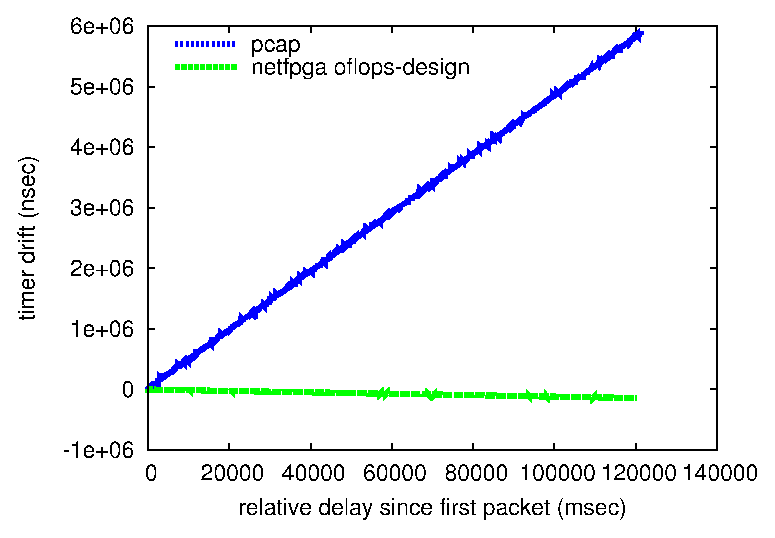
\includegraphics[width=0.99\textwidth]{timer_precision} 
 \caption{Evaluating timestamping precision using a DAG card.}
\label{fig:timestamping}
\end{minipage}
\end{figure}

The \oflops design philosophy aims to develop a low overhead abstraction layer
that allows interaction with an OpenFlow-enabled device over multiple data
channels.  The platform provides a unified system that allows developers to
control and receive information from multiple control sources: data and control
channels as well as SNMP to provide specific switch-state information.
For the development of measurement experiments over \oflops, the platform
provides a rich, event-driven, API that allows developers to handle events
programatically in order to implement and measure custom controller
functionality. The current version is written predominantly in C. Experiments
are compiled as shared libraries and loaded at run-time using a simple
configuration language, through which experimental parameters can be defined.
A schematic of the platform is presented in Figure~\ref{fig:oflops_design}.
Details of the \oflops programming model can be found in the API manual
\cite{oflops-manual}.

The platform is implemented as a multi-threaded application, to take
advantage of modern multicore environments. To reduce latency, our design
avoids concurrent access controls: we leave any concurrency-control complexity 
to individual module implementations. \oflops consists of the following five threads, 
each one serving specific type of events:\\
\textbf{1. Data Packet Generation}: control of data plane traffic generators.\\
\textbf{2. Data Packet Capture}: data plane traffic interception.\\
\textbf{3. Control Channel}: controller events dispatcher.\\
\textbf{4. SNMP Channel}: SNMP event dispatcher.\\
\textbf{5. Time Manager}: time events dispatcher.

\oflops provides the ability to control concurrently multiple data
channels to the switch. Using a tight coupling of the data and control 
channels, programers can understand the impact of the measurement
scenario on the forwarding plane. To enable our platform to run on
multiple heterogeneous platforms, we have integrated support for
multiple packet generation and capturing mechanisms. For the packet
generation functionality, \oflops supports three mechanisms:
user-space, kernel-space through the pktgen module~\cite{pktgen}, and
hardware-accelerated through an extension of the design of the NetFPGA
Stanford Packet Generator~\cite{Covington09}.  For the packet
capturing and timestamping, the platform supports both the pcap
library and the modified NetFPGA design. Each approach provides
different precisions and different impacts upon the measurement
platform.

A comparison of the precision of the traffic capturing mechanisms is 
presented in Figure~\ref{fig:timestamping}. In this experiment we 
use a constant rate 100 Mbps probe of small packets for a two minute 
period. The probe is duplicated, using an optical wiretap with negligible 
delay, and sent simultaneously to OFLOPS and to a DAG card. In the figure, 
we plot the differences of the relative timestamp between each OFLOPS 
timestamping mechanism and the DAG card for each packet. From the figure, 
we see that the pcap timestamps drift by 6 milliseconds after 2 minutes.
On the other hand, the NetFPGA timestamping mechanism has a smaller
drift at the level of a few microseconds during the same period.

\section{Measurement setup}\label{sec:oflops-switches}

The number of \of-enabled devices has slowly increased recently, with switch and
router vendors providing experimental \of support such as prototype and
evaluation firmware. At the end of 2009, the \of protocol specification was
released in its first stable version 1.0~\cite{openflow-spec}, the first
recommended version implemented by vendors for production systems.
Consequently, vendors did proceed on maturing their prototype implementations,
offering production-ready \of-enabled switches today. Using \oflops, we evaluate
\of-enabled switches from three different switch vendors.  Vendor 1 has
production-ready \of support, whereas vendors 2 and 3 at this point only provide
experimental \of support.  The set of selected switches provides a
representative but not exhaustive sample of available \of-enabled
top-of-rack-style switching hardware. Details regarding the CPU and the size of
the flow table of the switches are provided in Table~\ref{tbl:switch_list}.

\of is not limited to hardware. The \of protocol reference is the software
switch, OpenVSwitch~\cite{openvswitch}, an important implementation for
production environments. Firstly, OpenVSwitch provides a replacement for the
poor-performing Linux bridge~\cite{bianco10}, a crucial functionality for
virtualised operating systems.  Secondly, several hardware switch vendors use
OpenVSwitch as the basis for the development of their own \of-enabled firmware.
OpenVSwitch development team has standardised a clean abstraction over the
control of the switch silicon (similar to linux HAL), which allows code reuse
over any forwarding entity that implements the switch abstraction. Thus, the
mature software implementation of the \of protocol is ported to commercial
hardware, making certain implementation bugs less likely to (re)appear.  In this
paper, we study OpenVSwitch alongside our performance and scalability study of
hardware switches. Finally, in our comparison we include the \of switch design
for the NetFPGA platform~\cite{openflow-netfpga}. This implementation is based
on the \of reference implementation, extending it with a hardware forwarding
design. 

\begin{table}[h!]
  \begin{center}
{
  \begin{tabular}{ |c | c | c | }
    \hline                        
    \textbf{Switch} & \textbf{CPU} & \textbf{Flow table size} \\
    \hline  
    Switch1 & PowerPC 500MHz & 3072 mixed flows \\
    \hline  
    Switch2 & PowerPC 666MHz & 1500 mixed flows \\
    \hline  
    Switch3 & PowerPC 828MHz & 2048 mixed flows \\
    \hline  
    OpenVSwitch & Xeon 3.6GHz & 1M mixed flows \\
    \hline  
    NetFPGA &  DualCore 2.4GHz & 32K exact \& 100 wildcard \\
    \hline 
  \end{tabular}  

}
\end{center}
\caption{OpenFlow switch details.}
\label{tbl:switch_list}
\end{table}

In order to conduct our measurements, we setup \oflops on a dual-core
2.4GHz Xeon server equipped with a NetFPGA card.
For all the experiments we utilize the NetFPGA-based packet generating and 
capturing mechanism. 1Gbps control and data channels are connected directly 
to the tested switches. We measure the processing delay incurred by the 
NetFPGA-based hardware design to be a near-constant $900$ nsec independent 
of the probe rate.

%%%%%%%%%%%%%%%%%%%%%%%%%%%%%%%%%%%%%%%%%%%%%%%
\section{Switch Evaluation}\label{sec:oflops-result}
%%%%%%%%%%%%%%%%%%%%%%%%%%%%%%%%%%%%%%%%%%%%%%%%

% In this section we present a set of tests performed by \oflops to
% measure the behavior and performance of \of-enabled
% devices. These tests target (1) the \of packet processing 
% actions, (2) the update rate of the \of flow table along with 
% its impact on the data plane, (3) the monitoring capabilities provided 
% by \of, and (4) the impact of interactions between different 
% \of operations.

As for most networking standards, there are different ways to implement a
given protocol based on a paper specification. \of is not different in this
regard. The current reference implementation is defined through OpenVSwitch
\cite{openvswitch}. However, different software and hardware implementations may
not implement all features defined in the OpenVSwitch reference, or they may
behave in an unexpected way. In order to understand the behaviour of switch \of
implementation, we develop a suite of measurement experiments to
benchmark the functionality of the elementary protocol interactions.  These
tests target (1) the \of packet processing actions~\ref{sec:result-packets}, (2)
the packet interception and packet injection functionality of the
protocol~\ref{sec:result-pktin}, (3) the update rate of the \of flow table along
with its impact on the data plane,~\ref{sec:result-rate} (4) the monitoring
capabilities provided by \of, and (5) the impact of interactions between
different \of operations.


\subsection{Packet modifications}\label{sec:results-packets}

The \of specification \cite{openflow-spec} defines ten packet
modification actions which can be applied on incoming
packets. Available actions include modification of MAC, IP, and VLAN
values, as well as transport-layer fields. A flow definition can
contain any combination of them. The left column of
Table~\ref{tbl:feature_delay} lists the packet fields that can be
modified by an \of-enabled switch.
These actions are used by network devices such as IP routers (e.g.,
rewriting of source and destination MAC addresses) and NAT (rewriting
of IP addresses and ports). Existing network equipment is tailored to
perform a subset of these operations, usually in hardware to sustain
line rate. On the other hand, how these operations are to be used is
yet to be defined for new network primitives and applications, such as
network virtualization, mobility support, or flow-based traffic
engineering.

% Explain how we measure the time taken to perform the modification.
To measure the time taken by an OpenFlow implementation to modify a
packet field header, we generate from the NetFPGA card UDP packets of
100 bytes at a constant rate of 100Mbps (approx. 125 Kpps). 
This rate is high enough to give statistically significant results in
a short period of time, without causing any packet queuing for any of the
switches.  The flow table is initialized with a flow that
applies a specific action on all probe packets and the processing
delay is calculated using the transmission and receipt timestamps,
provided by the NetFPGA.
%, while also low enough so that the impact of
%queuing at the network interface cards can be ignored. 
%Each packet is
%timestamped when leaving the NetFPGA card. The packet then arrives at
%the OpenFlow switch via a direct 1Gbps Ethernet link, the switch
%matches the packet against the flow table, and sends it back to the
%NetFPGA card where it is timestamped again.

\begin{table*}[tb]
\begin{flushleft}
        \begin{tabular}[t]{ |l | c | c | c || c | c | c  || c | c | c | }
          \hline                       
          Mod. type & \multicolumn{3}{|c|}{Switch 1} & \multicolumn{3}{|c|}{ovs} &
          \multicolumn{3}{|c|}{Switch 2} \\ 
          \hline                       
          & med & sd & loss\%  & med & sd & loss\% & med & sd & loss\%\\
          \hline  
          Forward & 4 & 0 & 0 & 35 & 13 & 0& 6 & 0 & 0 \\
          \hline  
          MAC addr. & 4 & 0 & 0 & 35 & 13 & 0& 302 & 727 & 88\\
          \hline  
          IP addr. & 3 & 0 & 0 & 36 & 13 & 0 & 302 & 615 & 88\\
          \hline  
          IP ToS & 3 & 0 & 0 & 36 & 16 & 0 & 6 & 0 & 0\\
          \hline  
          L4 port & 3 & 0 & 0 & 35 & 15 & 0 & 302 & 611 &  88\\
          \hline  
          VLAN pcp & 3 & 0 & 0 & 36 & 20 & 0 & 6 & 0 & 0\\
          \hline  
          VLAN id & 4 & 0 & 0 & 35 & 17 & 0 & 301 & 610 & 88\\
          \hline  
          VLAN rem. & 4 & 0 & 0 & 35 & 15 & 0 & 335 & 626 & 88\\
      \hline
    \end{tabular}
   \begin{tabular}[t]{ |l | c | c | c || c | c | c | }
          \hline                       
          Mod. type & \multicolumn{3}{|c|}{Switch 3} & \multicolumn{3}{|c|}{NetFPGA}\\ 
          \hline                       
          & med & sd & loss\%  & med & sd & loss\% \\
          \hline  
          Forward & 5 & 0 & 0 & 3 & 0 & 0 \\
          \hline  
          MAC addr. & - & - & 100 & 3 & 0 & 0 \\
          \hline  
          IP addr. & - & - &  100 & 3 & 0 & 0 \\
          \hline  
          IP ToS & - & - & 100 & 3 & 0 & 0 \\
          \hline  
          L4 port & - & - & 100 & 3 & 0 & 0 \\
          \hline  
          VLAN pcp & 5 & 0 & 0 & 3 & 0 & 0 \\
          \hline  
          VLAN id & 5 & 0 & 0 & 3 & 0 & 0  \\
          \hline  
          VLAN rem. & 5 & 0 & 0 & 3 & 0 & 0 \\
      \hline
    \end{tabular}
 
\caption{Time in $\mu$s to perform individual packet modifications and packet
loss. Processing delay indicates whether the operation is
  implemented in hardware (\textless10$\mu$s) or performed by the CPU (\textgreater10$\mu$s).}
  \label{tbl:feature_delay}
\end{flushleft}
\end{table*}
% What the table shows...
Evaluating individual packet field modification,
Table~\ref{tbl:feature_delay} reports the median difference between
the generation and capture timestamp of the measurement probe along
with its standard deviation and percent of lost packets.

We observe significant differences in the performance of the hardware
switches due in part to the way each handles packet
modifications. Switch1, with its production-grade implementation,
handles all modifications in hardware; this explains its low packet
processing delay between 3 and 4 microseconds. On the other hand,
Switch2 and Switch3 each run experimental firmware providing only
partial hardware support for \of actions. Switch2 uses the switch
CPU to perform some of the available field modifications, resulting in two orders
of magnitude higher packet processing delay and variance.
Switch3 follows a different approach: All packets of flows with
actions not supported in hardware are silently discarded. The
performance of the OpenVSwitch software implementation lies between
Switch1 and the other hardware switches.  OpenVSwitch fully implements
all \of actions. However, hardware switches outperform
OpenVSwitch when the flow actions are supported in hardware.
% than the delay of the hardware path of the hardware switches,
% dominated by the NIC-CPU latency.
%
% For example, the time of an ensemble of modifications is dictated by the
% maximum time across all modifications.\todo{Last sentence is reported to be
% misleading by the reviewers}
% Furthermore, we notice that for switch1 and openvswitch there is
% limit of 7 actions, which may enveil similrities in the code base.
% From the results presented in Table~\ref{tbl:feature_delay}, we can
% already conclude that an experimental hardware-based OpenFlow
% implementation is likely to deliver poor performance compared to a
% mature software-based implementation running on commodity PC
% hardware

We conducted a further series of experiments with variable numbers of packet
modifications as flow actions. We observed, that the combined processing time of
a set of packet modifications is equal to the highest processing time across all
individual actions in the set. Furthermore, we notice that for Switch1 and 
OpenVSwitch there is a limit of 7 actions, which potentially exposes some
relation in the code base.

\subsection{Traffic interception and injection}\label{sec:results-pktin}

\begin{figure}[ht]
  \begin{center}
    \subfigure[Packet in message latency]
    {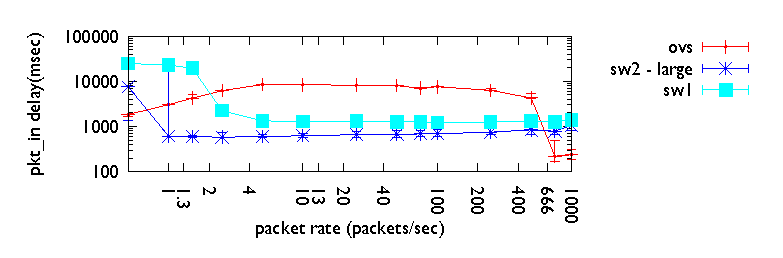
\includegraphics[width=0.99\textwidth]{pkt_in_delay}}
    \subfigure[Packet out message latenct]
	{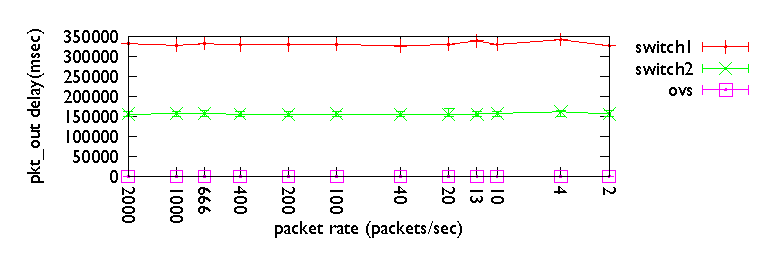
\includegraphics[width=0.99\textwidth]{pkt_out_delay}}
  \end{center}
  \caption{Latency to intercept or inject a packet using the \of protocol}
  \label{fig:pkt_in_out_delay}
\end{figure}

\of protocol permits a controller to intercept or inject traffic over the
control plane. This functionality permits to \of controller applications to be reactive and
handle traffic on a per-flow basis. Packet injection allows the controller to
interact with connected network hosts. The interception mechanism in \of has
been reported in the initials deployments of the protocol to cause significant
slow-down in the control plane and led to switch disconnection at high packet
rate~\cite{Kobayashi:vn}. This is a direct consequence of the silicon design in
current \of switches, that develop such functionality over a low-frequency
exception notification channel. In order to characterise this functionality, we
develop a simple experiment using \oflops that sends packet\_in messages over the
control channel at different rates
and measure the latency of the switch to process them. In
Figure~\ref{fig:pkt_in_out_delay}, we plot the latency induced on packets both
for Packet\_in and Packet\_out messages. We omit in this experiment Switch 3 as
this functionality cause high CPU utilisation and after a few seconds made the
switch unresponsive. For packet\_out messages, the switches rate limit through
the TCP rate control mechanism the rate of messages received and as a result they
provide a constant performance. For packet\_in messages, we observe a diverse
behaviour between hardware switches at high packet rates. For Switch 1, packet
loss and latency gets high for traffic rates above 400 packets per second.
Additionally, we noticed that the switch is able to process a maximum of 500
packets/sec. For Switch 2 latency and packet loss are significantly lower and
stable. Switch 2 faced problem to process packets at high rates, over 2000
packets per second. OpenVSwitch, has a high but stable latency for any tested
data rates. 

\subsection{Flow table update rate}\label{sec:results-rate}

% So far, we get packet modification primitives and the expected performance that software/hardware can/should deliver.
% 
\begin{figure}[ht]
  \begin{center}
    \subfigure[OpenVSwitch (log-log scale)]
    {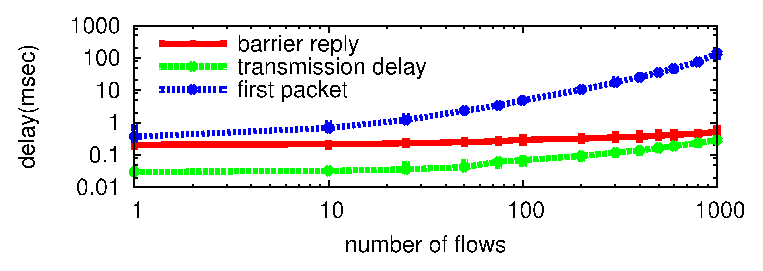
\includegraphics[width=0.99\textwidth]{openvswitch_mod_flow_exact_comparison}}
    \subfigure[Switch1 (log-log scale)]
	{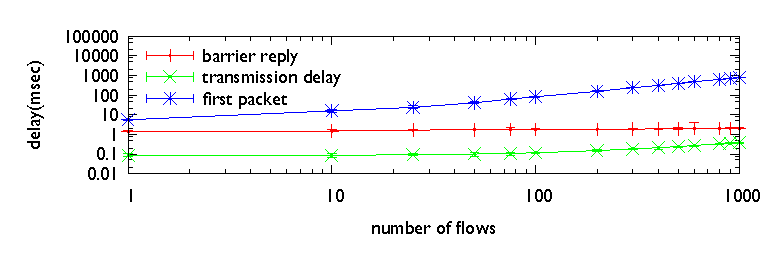
\includegraphics[width=0.99\textwidth]{nec_mod_flow_exact_comparison}}
  \end{center}
  \caption{Flow entry insertion delay: as reported using the
    \texttt{barrier} notification and as observed at the data
    plane.}
  \label{fig:flow_insertion_comparison}
\end{figure}

The flow table is a central component of an OpenFlow switch and is the
equivalent of a Forwarding Information Base (FIB) on routers. Given the
importance of FIB updates on commercial routers, e.g., to reduce the impact of
control plane dynamics on the data plane, the FIB update processing time of
commercial routers provide useful reference points and lower bounds for the time
to update a flow entry on an OpenFlow switch. The time to install a new entry on
commercial routers has been reported in the range of a few hundreds of
microseconds~\cite{shaikh-igp}.

OpenFlow provides a mechanism to define barriers between sets of
commands: the \texttt{barrier} command. According to the OpenFlow
specification~\cite{openflow-spec}, the barrier command is a way to be
notified that a set of OpenFlow operations has been completed. Further, 
the switch has to complete the set of operations issued prior to the barrier 
before executing any further operation. If the OpenFlow implementations 
comply with the specification, we expect to receive a barrier notification for 
a flow modification once the flow table of the switch has been updated, 
implying that the change can be seen from the data plane.

We check the behavior of the tested OpenFlow implementations,
finding variation among them. For OpenVSwitch and Switch1,
Figure~\ref{fig:flow_insertion_comparison} shows the time to install a
set of entries in the flow table. The NetFPGA-based switch results
(not reported) are similar to those of Switch1, while Switch2 and Switch3 
are not reported as this OpenFlow message is not supported by the firmware. 
For this experiment, \oflops relies on a stream of packets of 100 bytes at
a constant rate of 10Mbps that targets the newly installed flows in a
round-robin manner. The probe achieves sufficiently low inter-packet
periods in order to measure accurately the flow insertion time.
%With such a probe stream, we obtain an inter-packet
%period of less than 100$\mu$s, adequate for measuring any change in
%the flow-insertion time.

In Figure~\ref{fig:flow_insertion_comparison}, we show three different
times. The first, {\it barrier notification}, is derived by measuring the time 
between when the \textbf{first insertion command} is sent by the \oflops 
controller and the time the barrier notification is received by the PC. The 
second, {\it transmission delay}, is the time between the first and 
last flow insertion commands are sent out from the PC running \oflops. 
The third, {\it first packet}, is the time between the \textbf{first insertion
 command} is issued and a packet has been observed for the last of
the (newly) inserted rules. For each configuration, we run the
experiment 100 times and Figure~\ref{fig:flow_insertion_comparison}
shows the median result as well as the $10^{th}$ and $90^{th}$ percentiles 
(variations are small and cannot be easily viewed).
%\todo{point that the error
%  bounds are tight and cannot easily viewed on the graph}

From Figure~\ref{fig:flow_insertion_comparison}, we observe that even
though the {\it transmission delay} for sending flow insertion commands 
increases with their number, this time is negligible when compared with 
data plane measurements ({\it first packet}). Notably, the {\it barrier notification} 
measurements are almost constant, increasing only as the transmission delay 
increases (difficult to discern on the log-log plot) and, critically, this operation 
returns before any {\it first packet} measurement. This implies that the way
the {\it barrier notification} is implemented does not reflect the time when 
the hardware flow-table has been updated.

In these results we demonstrate how \oflops can compute per-flow
overheads. We observe that the flow insertion time for Switch1
starts at $1.8$ms for a single entry, but converges toward an
approximate overhead of $1$ms per inserted entry as the number of
insertions grows.

%%%%%%%%%%%%%%%%%%%%%%%%%%%%%%%%%%%%%%%%%%%%%%
\subsubsection*{Flow insertion types}
%%%%%%%%%%%%%%%%%%%%%%%%%%%%%%%%%%%%%%%%%%%%%%

\begin{figure}[h]
  \begin{center}
    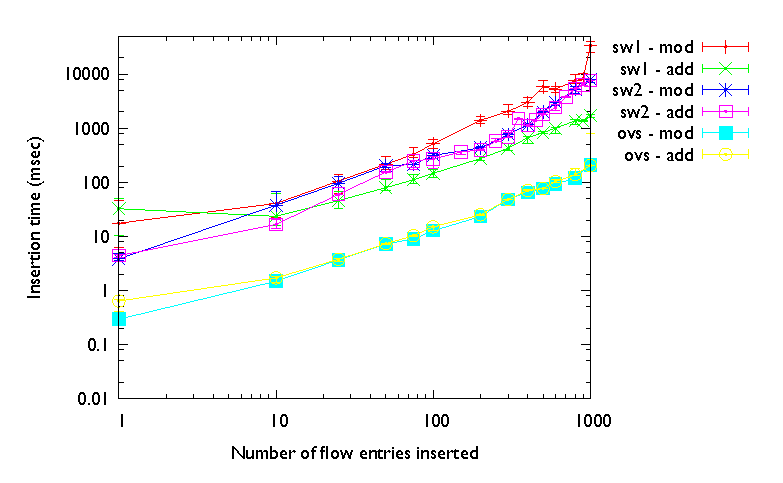
\includegraphics[width=0.80\textwidth]{flow_insertion_delay}
  \end{center}
  \caption{Delay of flow insertion and flow modification, as observed
    from the data plane (log-log scale).}
  \label{fig:flow_insertion_delay}
\end{figure}

We now distinguish between flow insertions and the modification of existing flows.  
With OpenFlow, a flow rule may perform exact packet matches or use wild-cards to 
match a range of values. Figure~\ref{fig:flow_insertion_delay} compares the flow
insertion delay as a function of the number of inserted entries. This is done for the 
insertion of new entries and for the modification of existing entries.

These results show that for software switches that keep all entries in memory, the 
type of entry or insertion does not make a difference in the flow insertion time.
Surprisingly, both Switch1 and Switch2 take more time to modify existing flow entries 
compared to adding new flow entries.  For Switch1, this occurs for more than 10 new 
entries, while for Switch2 this occurs after a few tens of new entries.
After discussing this issue with the vendor of Switch2, we came to the
following conclusion: as the number of TCAM entries increases, updates
become more complex as they typically requires re-ordering of existing
entries.

Clearly, the results depend both on the entry type and implementation.
For example, exact match entries may be handled through a hardware or
software hash table. Whereas, wild-carded entries, requiring support
for variable length lookup, must be handled by specialized memory
modules, such as TCAM. With such possible choices and range of
different experiments, the flow insertion times reported in
Figure~\ref{fig:flow_insertion_delay} are not generalizable, but
rather depend on the type of insertion entry and implementation.

% %%%%%%%%%%%%%%%%%%%%%%%%%%%
\subsection{Flow monitoring}\label{sec:results-monitoring}
% %%%%%%%%%%%%%%%%%%%%%%%%%%%

The use of OpenFlow as a monitoring platform has already been
suggested for the applications of traffic matrix
computation~\cite{opentm-pam,tm-presto} and identifying large traffic
aggregates~\cite{openflow-measurement-hotice}. To obtain direct
information about the state of the traffic received by an OpenFlow
switch, the OpenFlow protocol provides a mechanism to query traffic
statistics, either on a per-flow basis or across aggregates matching
multiple flows and supports packet and byte counters. 
%The result of a query returns packet and byte
%counters, either for the matched flows individually or for the
%aggregate.

We now test the performance implications of the traffic statistics reporting 
mechanism of OpenFlow. Using \oflops, we install flow entries that match 
packets sent on the data path. Simultaneously, we start sending flow statistics 
requests to the switch. Throughout the experiment we record: the delay getting 
a reply for each query, the amount of packets that the switch sends for each 
reply and the departure and arrival timestamps of the probe packets.

Figure~\ref{fig:stat_request} reports the time to receive a flow
statistics reply for each switch, as a function of the request
rate. Despite the rate of statistics requests being modest, quite high
CPU utilization results for even a few queries per second being
sent. Figure~\ref{fig:stat_request} reports the switch-CPU utilization
as a function of the flow statistics inter-request time. Statistics
are retrieved using SNMP. Switch3 is excluded for lack of SNMP
support.

\begin{figure}[h]
  \begin{center}
    \subfigure[Reply time.]
    {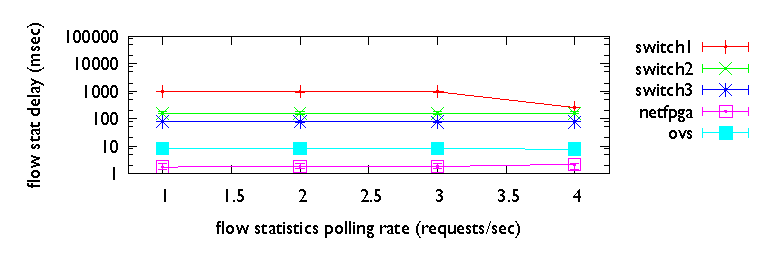
\includegraphics[width=0.99\textwidth]{flow_stats_delay}}
    \subfigure[CPU utilization.]
      {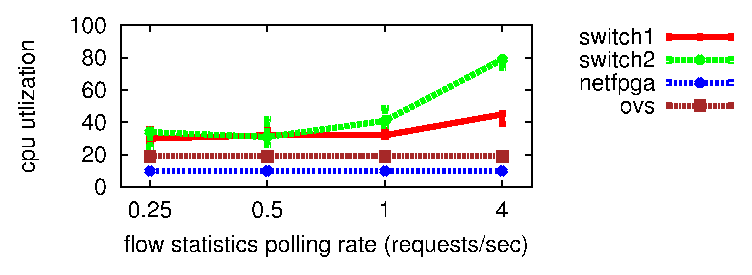
\includegraphics[width=0.99\textwidth]{flow_stats_cpu}\label{fig:stat_request_cpu}}
  \end{center}
  \caption{Time to receive a flow statistic (median) and corresponding CPU utilization.}
  \label{fig:stat_request}
\end{figure}

From the flow statistics reply times, we observe that all switches have (near-)constant 
response delays: the delay itself relates to the type of switch.
As expected, software switches have faster response times than
hardware switches, reflecting the availability of the information in memory
without the need to poll multiple hardware counters. These consistent response
times also hide the behavior of the exclusively hardware switches
whose CPU time increases proportionally with the rate of requests.  We
observe two types of behavior from the hardware switches: the switch
has a high CPU utilization, answering flow-stats requests as fast as
possible (Switch2), or the switch delays responses, avoiding
over-loading its CPU (Switch1). Furthermore, for Switch1,
we notice that the switch is applying a pacing mechanism on its
replies. Specifically, at low polling rates the switch splits its
answer across multiple TCP segments: each segment containing statistics for a
single flow.  As the probing rate increases, the switch
will aggregate multiple flows into a single segment. This suggests that 
independent queuing mechanisms are used for handling flow statistics 
requests. Finally, neither software nor NetFPGA switches see an 
impact of the flow-stats rate on their CPU, thanks to their significantly 
more powerful PC CPUs (Table~\ref{tbl:switch_list}).

%%%%%%%%%%%%%%%%%%%%%%%%%%%%%%%%%%%%%%%%%
\subsection{OpenFlow command interaction}\label{sec:results-interactions}
%%%%%%%%%%%%%%%%%%%%%%%%%%%%%%%%%%%%%%%%%

% why is it important this experiment

An advanced feature of the OpenFlow protocol is its ability to
provide applications with, e.g., flow arrival notifications from the 
network, while simultaneously providing fine-grain control of 
the forwarding process. This permits applications to adapt
in real time to the requirements and load of the
network~\cite{plug_n_serv,Yap09}. Under certain OpenFlow usage
scenarios, e.g., the simultaneous querying of traffic statistics and
modification of the flow table, understanding the behavior of the data
and control plane of OpenFlow switches is difficult without advanced
measurement instrumentation such as the one provided by \oflops. 
Through this scenario, we extend Section~\ref{sec:results-rate} to show 
how the mechanisms of traffic statistics extraction and table manipulation 
may interact. Specifically, we initialize the flow table with 1024 exact
match flows and measure the delay to update a subset of 100 flows. 
Simultaneously, the measurement module polls the switch for full table 
statistics at a constant rate. The experiment uses a constant rate 10Mbps 
packet probe to monitor the data path, and polls every 10 seconds for SNMP 
CPU values.

\begin{figure}[t!!]
  \begin{center}
    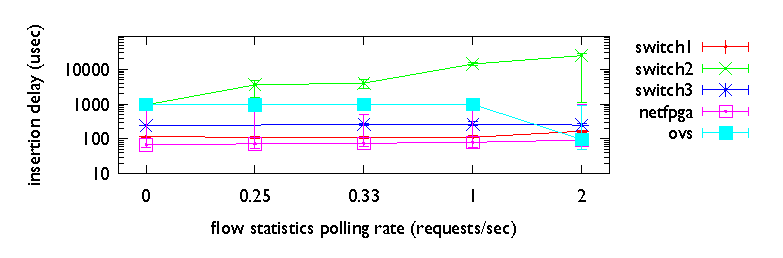
\includegraphics[width=0.99\textwidth]{interaction_test}
  \end{center}
  \caption{Delay when updating  flow table while the controller polls
    for statistics.}
  \label{fig:interaction_test}
\end{figure}

In this experiment, we control the probing rate for the flow statistics 
extraction mechanism, and we plot the time necessary for the modified 
flows to become active in the flow table. For each probing rate, we
repeat the experiment 50 times, plotting the median, $10^{th}$ and 
$90^{th}$ percentile. In Figure~\ref{fig:interaction_test} we can see
that, for lower polling rates, implementations have a near-constant
insertion delay comparable to the results of Section~\ref{sec:results-rate}.
For higher probing rates on the other hand, Switch1 and Switch3 do 
not differ much in their behavior. In contrast, Switch2 exhibits a noteworthy 
increase in the insertion delay explained by the CPU utilization increase
incurred by the flow statistics polling (Figure~\ref{fig:stat_request_cpu}). Finally,
OpenVSwitch exhibits a marginal decrease in the median insertion delay
and at the same time an increase in its variance. We believe this behavior 
is caused by interactions with the OS scheduling mechanism: the constant 
polling causes frequent interrupts for the user-space daemon of the switch, 
which leads to a batched handling of requests.

% \subsection{Timer precision} As part of each flow modification the
% protocol defines that the controller is able to define an expiration
% value for the flow. When a flow is expired, it is removed from the
% table. The protocol supports two different mechanism to define the
% timeout of a flow. Timeouts can be defined either based on the
% insertion time or the last time that the flow was used. The
% definition of the precision of this mechanism would be beneficial to
% applications that require high precision from the routing mechanism.
% In order to address the precision of the mechanism we are developing
% an experiment over the \oflops platform. The experiment utilizes 2
% ports of the switch and a single measurement probe with constant all
% field and random destination IP. During initialization the switch is
% initialized with a single wildcard flow that output packets to port
% 2. At time t=10 sec since the start of the experiment the controller
% sends an ensemble of exact match rules with different destination
% IP's and a hard expiration delay of 10 seconds. All the flows of the
% ensemble contain a single action which outputs packets on port
% 1. The experiments terminate when we receive all the flow expiration
% messages from the switch. During the experiment we log for each flow
% the time at which we received the first and last packet of the
% measurement probe for each destination IP. In the experiment we
% export as a parameter the number of flows send to the switch. For
% each number of flows we rerun the experiment for 20 times. In Figure
% \ref{fig:timer_precision} we present the results of our
% experiment. For each number of flows we plot an errorbar with the
% minimum, maximum and medium of the maximum error in the timeout of a
% flow based on the results of the packet timestamps of the
% measurement probe.
% \subsubsection*{Results}
% \subsection{Simulating a reactive switch} Simulate a Nox like
% behaviour and measure the time send at each stage of the flow
% insertion process. export as parameters the rate we send packets and
% the number of flows inserted.
% \subsubsection*{Results}
% LocalWords:  OpenFlow Oflops IP VLAN balancers SDNs virtualization NetFPGA th
% LocalWords:  UDP Mbps Gbps multiport timestamp OpenVSwitch dev dest src addr

% LocalWords:  NIC ToS TCP pcp interpacket TCAM lookup SNMP CPUs parameterising


\section{\of Macro-experimentation} \label{sec:sdnsim-intro}

% SDN paradigm provides functional evolution in a network that is backward
% compatible with existing network systems. The evolution is achieved through
% network control distribution to external programmable units. In order to have 
% effective control delegation, an SDN protocol
% \textit{must} provide sufficient forward plane control and feedback to the 
% controlling entity. So far the trend in \of design is to aggregate control in a single
% control unit, in order to have a single point of control in the network. This
% aggregation permits on one hand to achieve higher optimality in forwarding
% policy, while on the other hand the logic can be developed in richer programming
% environments, than the embedded systems usually found in current network
% devices.

\oflops, along with cbench~\cite{cbench}, provide a sufficient set of tools to
profile functionality of \of building blocks and understand the low-level
capabilities. Nonetheless, the provided measurements are not sufficient to
establish models that can predict network performance with tight error bounds.
The distribution of control functionality over multiple functional units, in
conjunction with the diverse behaviour of \of switch and controlling platforms,
reduce the ability to develop analytical models that can estimate the behaviour
of an SDN design. In order to reason on performance, as well as correctness,
developers have to revert to an experimental approach.  In the related
literature on network evaluation there have been two main experimental
mechanisms: \emph{realistic-testbed} and \emph{simulation}.

Realistic testbeds try to reconstruct in full detail the properties of the
deployment environment. This approach provides an optimal measurement
environment with complete control over the parameter of the experiment, but has
a significant overhead in terms of resource requirements and configuration time,
which scales badly as the experiment size increases.  Setting up a realistic
testbed for datacenter networking requires a large number of machines and
network devices with identical functionality in respect to the deployment
environment, interconnection planning and careful metrication and analysis of
the resulting system. In an effort to improve the scalability issues of
realistic testbeds, the research community has established a number of shared
testbeds. Such testbeds employ techniques such as virtualization and statistical
multiplexing, and provide low-level user access to sizable
infrastructures~\cite{planetlab,emulab}.  Nontheless, such platform are not
always a good fit for network experiments. Resource control
is reduced and measurement noise, due to infrastructure sharing, is not always
easy to detect and remove. 

In the simulation approach, researchers replace parts of the functionality of
the system by simpler models~\cite{Varga2008,issariyakul2012}.  Such
approaches aim to reduce the complexity of an experiment for large scale
networks, but faces a number of limitation.  Firstly, the fidelity of the
results depends greatly on the validity of the model assumptions. Secondly, in
order to simulate network experiments, users usually need to readjust the logic
of their experiments in order to fit the abstraction of the underlying models.
For example, POSIX socket-based controllers need to modify the control channel
abstraction in order to match the API of the simulation platform,
while forwarding plane traffic may have to be translated in a stochastic model. 

\sdnsim~\footnote{\sdnsim is under GPL licence and can be downloaded from
  \url{http://github.com/crotsos/sdnsim/}} is a novel network experimentation
framework, that bridges the two aforthmentioned approaches. The framework is
written in OcaML, a high performance functional language, and extends the
functionality of the Mirage~\footnote{\mirageurl} library OS. Developers can
implement the desired network functionality over the mirage OS abstraction, and
at the compilation step produce a number of different experimentation target.
\sdnsim provides two experimentation options: \emph{Simulation}, transforms
the high level logic in NS-3~\cite{ns3} simulation, and \emph{Emulation},
translates the high level logic of each host into Xen-based interconnected DomU
VMs. In addition, because \sdnsim reuse the abstraction provided by the Mirage
OS, functionality can also be translated to any of the available output of
the Mirage OS.

\section{Mirage Library OS} \label{sec:mirage-intro}

\begin{figure}
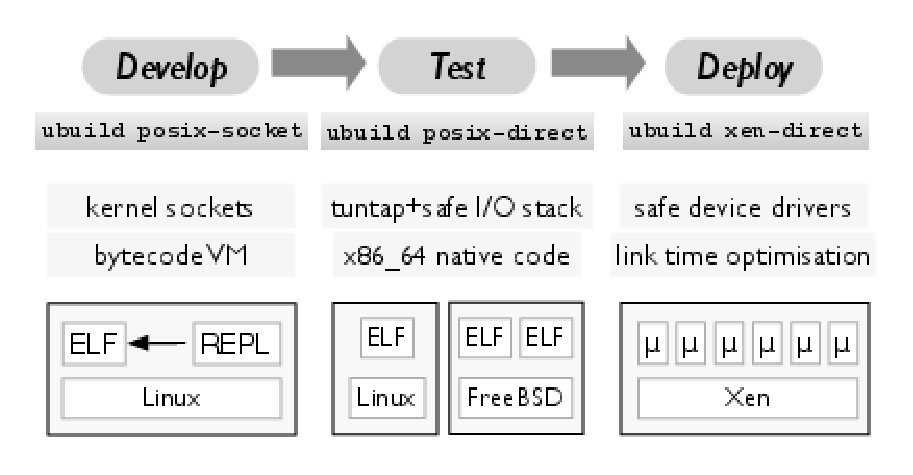
\includegraphics[width=0.9\textwidth]{mirage-toolchain}
\caption{Specialising a \mirage application through recompilation alone, from
  interactive UNIX Read-Eval-Print Loop, to reduce dependency on the host
  kernel, and finally a unikernel VM.}
\label{fig:mirage-toolchain}
\end{figure}

% Cloud computing has revolutionized the way the business use IT infrastructures
% as well as the way we develop distributed computing applications. The
% abstraction is straightforward. A third party entity takes responsibility to
% maintain a datacenter. This infrastructure, is partitioned into smaller virtual
% computational units which clients can rent in order to run their applications.
% The elegance of this model is based on simplicity of the abstraction that the
% cloud provider provides to the user and the ability to port existing services
% running on a personal computer or a server to the cloud platform. 

% Although the simplicity of the exposed abstraction, the cloud architecture
% consist of a complex set of processing layers. A single application VM would
% include: i) the virtualization runtime layer, ii) the guest OS kernel layer,
% iii) A language runtime layer (POSIX, JVM etc.) iv) user-space
% thread layer. This layer complexity, although it provides excellent backwards
% compatibility for existing datacenter applications, it makes the process of
% optimisation, debugging as well as security difficult, while there is a
% significant overlap on the functionality provided by each layer. 

Mirage is a cloud service development framework written in OCaml. Mirage
applications are single purpose appliances that are compile-time specialised
into standalone kernels deployable on the Xen platform. The aim of the framework
is to provide small size cloud OS images that are efficient and secure.  In
order to achieve this, Mirage revisits the idea of library OS; OS functionality
is separated into logical modules and added to an appliance only if the code
expresses an explicit dependency.  As a result, Mirage can generate small size
VM images with very fast boot times.  Furthermore, using OCaml, a type-safe
functional language, the framework is able to mitigate a number of security
attacks to applications.

Mirage executes OCaml code using a specialised language runtime modified in two
key areas: \textit{memory management} and \textit{concurrency}.  Since Mirage
applications are single process VMs, traditional complex memory virtualisation
and Address Space Randomisation (ASR) mechanisms are removed from the
architecture.  Mirage applications use a single address space, separated between
the text and data section of the program and the runtime heap. In addition,
since the program code is immutable during runtime, Mirage locks write access to
executable memory space, thus mitigating buffer overflow attacks.  Finally, in
order to improve performance for our system, Mirage provides a memory-safe
zero-copy mechanism and exposes applications to the memory space of the shared
memory ring.

In terms of concurrency, Mirage uses  the Lwt cooperative threading library
abstraction~\cite{lwt}. Lwt provides an OCaml syntax extension that can annotate
blocking IO and internally evaluate blocking functions into event
descriptors to provide straight-line control flow for the developer.  Written in
pure OCaml, Lwt threads are heap-allocated values, with only the thread main
loop requiring a C binding to poll for external events.  Mirage provides an
evaluator that uses Xen polling to listen for events and wake up lightweight
threads. The VM is thus either executing OCaml code or blocked, with no internal
preemption or asynchronous interrupts. The main thread repeatedly executes until
it completes or throws an exception, and the domain subsequently shuts down with
the VM exit code matching the thread return value.  A useful consequence is that
most scheduling and thread logic is contained in an application library, and can
thus be modified by the developer as they see fit. 

Mirage OS provides a simple API to applications developers, sufficient for
systems programming. This functionality is implemented by two core modules,
named \textit{Net} and \textit{OS}, which expose a minimum API to the network
and the device management stack.  The simplicity of the OS and Net modules,
permit Mirage to compile code to other target backends, apart from the Xen
platform. Specifically, Mirage can generate UNIX binaries, using both the POSIX
library network functionality and raw sockets, and even Javascript executables
that run in a browser. There is also currently an effort to port Mirage in the
FreeBSD kernel as well as over the BareMetalOS~\cite{baremetalOS}, an assembly OS.
The diverse set of deployment backends, provides  a sufficient environment for
test and optimization, as depicted in Figure~\ref{fig:mirage-toolchain}.
Developers build initially their core logic over the POSIX backend in order to
test the correctness of the code, then they can try their code over the Mirage
default network stack, to perform a small scale performance evaluation, and
finally they can synthesize the resulting deployable Xen Image.

% Although, OCaml is a functional language, it is able to generate highly
% performant binary code and application specific microbenchmarks has shown
% performance to be compare to C code implementations. 

\section{\sdnsim design} \label{sec:sdnsim-design}

\lstset{language=XML,
numberstyle=\footnotesize,
basicstyle=\ttfamily\footnotesize,
captionpos=b,
}
\begin{lstlisting}[caption={A sample \sdnsim configuration file interconnecting
  a server and a client host},label={lst:sdnsim-conf}]
<?xml version="1.0" encoding="ISO-8859-1"?>
<topology module="Simple_tcp_test" backend="ns3-direct" 
    duration="30">
  <modules>
    <library>lwt</library>
    <library>lwt.syntax</library>
    <library>cstruct</library>
    <library>cstruct.syntax</library>
    <library>mirage</library>
    <library>mirage-net</library>
    <library>pttcp</library>
  </modules>
  <node name="host1" main="host_inner"> 
    <param>1</param>
  </node>
  <node name="host2" main="host_inner"> 
    <param>2</param>
  </node>
  <link src="host1" dst="host2" delay="10" rate="100" 
    queue_size="100" pcap="false"/>
</topology>
\end{lstlisting}

\begin{figure}
\centering
\subfigure[NS3]{
 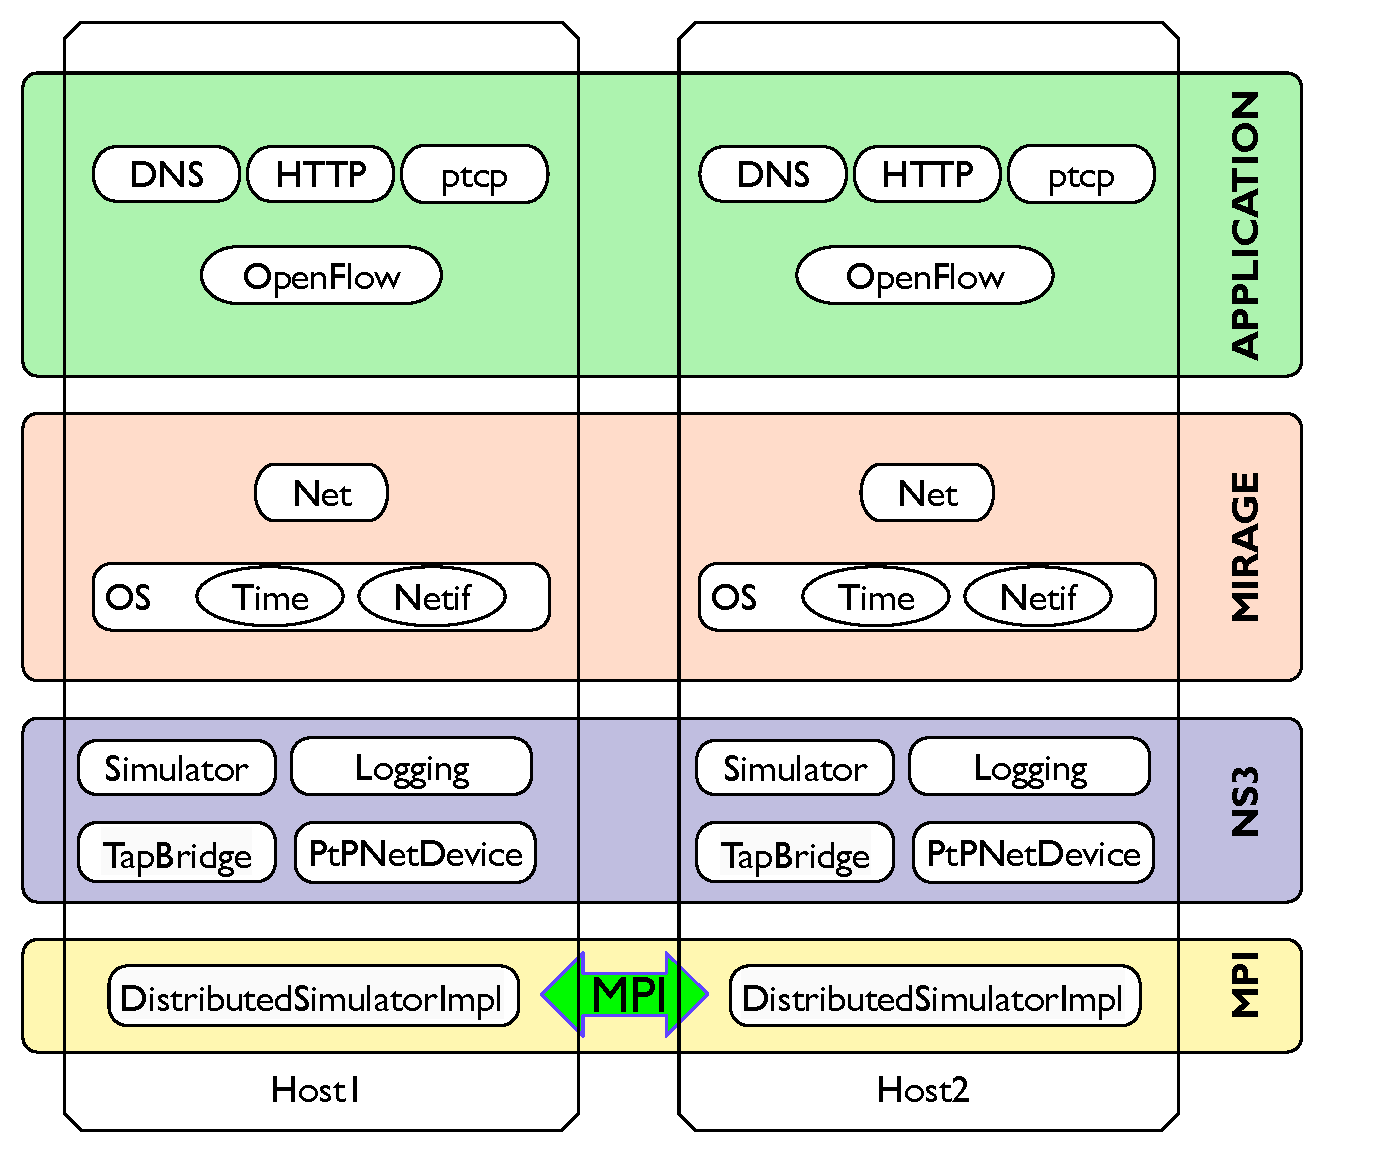
\includegraphics[width=0.45\textwidth]{sdnsim-arch-ns3}
 \label{fig:sdnsim-arch-ns3}}
\subfigure[Xen] {
 \includegraphics[width=0.45\textwidth]{sdnsim-arch-xen}
 \label{fig:sdnsim-arch-xen}}
\caption{\sdnsim host internal architecture: NS3
  simulation~\ref{fig:sdnsim-arch-ns3} and xen real-time
  emulation~\ref{fig:sdnsim-arch-xen}.}
\label{fig:sdnsim-arch}
\end{figure}

From the user perspective, \sdnsim consists of a single executable
that functions as an OCaml build system. Developers implement host
functionality as Mirage applications, and use a single XML file
to describe the network topology and assign functionality to network nodes.
A sample xml file is presented in Listing~\ref{lst:sdnsim-conf}. The
configuration describes a simple client~(host1)~-~server~(host2) configuration.
For an experiment definition, developers needs to define, at minimum,  the core
code module~(topology@module), the target executable~(topology@backend) and the
duration of the experiment~(topology@duration). In order to define a host,
\sdnsim uses a host xml entity. For each host users must define the host
name~(node@name) and the host main function~(node@main), while a number of named
parameters~(node/param) can be passed to the main function. Finally, developers
can define links between hosts~(link@src, link@dst) along with the
device~(link@queue\_size, link@pcap) and propagation properties~(link@rate,
link@delay), using the link xml entity. Links can be used also to integrate
external network interfaces in the simulation, in order to allow the experiment to
interact with entities outside of the experiment scope.

The functionality of a node in the \sdnsim platform can be split in 3 layers.  A
simple representation of the architecture of an \sdnsim host is depicted in
Figure~\ref{fig:sdnsim-arch}.  At the top layer of the host is the application
logic of the host. This layer is programmed by the developer, and define the
traffic load of the network and its forwarding logic. In order to allow
realistic traffic patterns, \sdnsim can reuse all the application protocol
libraries supported in the \mirage platform, namely DNS, HTTP, SSH and \of. For
the \of protocol library we modify the controller and switch functionality and
expose control hooks to define explicit lower bounds in processing latencies for
control and forward plane interactions.  This allows developers to inject
measurement results from \oflops and Cbench in their experiments.  Additionally,
we have re-implemented in OCaml the pttcp tcp test tool~\ref{pttcp}, in order to
allow model driven TCP and UDP traffic generation. 

In the middle layer of the host architecture, we reuse the network library and
the OS abstraction defined by the Mirage platform. These libraries are mapped in
the lower layer of the respective backend. Because these platforms aim to
develop an \of capable simulation platform, the main focus for the integration
between the two lower layer is the fidelity in network functionality and time
consistency. Currently, \sdnsim supports two backends, {\it NS3} and {\it Xen}.
In order to implement the lower layer integration, a different strategy has been 
followed for each backend. 

\subsection{Xen}

Mirage Xen Image, use a simple PV Boot
mechanism. The mechanism initializes a VM with a single virtual CPU, loads the
Xen event channel and jumps to the main function of the framework. The main function
enumerates IO devices and notifies the application and then progresses to the 
thread scheduler. As we have mentioned earlier, the threading
mechanism in Mirage is based on Lwt, a language extension which enables seamless
event-driven asynchronous programming. Using Lwt suntax, each closure can be
noted as blocking, and spawn a new lwt thread. At the lowest level, an lwt
thread is either tied to a blocking IO request, or a time dependent event. Using
this information, the scheduling logic works as follow: If no sleeping thread
is currently available to resume, the schduler calculates the
time left until the next time event and uses it as the timeout parameter for the
IO blocking method (named {\emph domainpoll}) provided by the Xen platform.
Domainpoll registers interest to the respective event handler and ask the Xen
scheduler to put the VM to sleep until either an event occurs or the timeout
option expires.Timing integration with the Xen platform is achieved through the Xen
shared\_info struct, a structure shared between the Dum0 and the DumU VMs. 
Network functionality is implemented over the IO interface of
the Xen NetFront driver.

\sdnsim uses Xen Managment API~(XenApi)to control the experimental
configuration over the Xen platform.
XenApi provides remote VM and resource allocation control of a Xen Domain. As a
result, \sdnsim is able to create and start VM instances, implements network
topologies through vif bridging in the Dum0 space, and assign link rate and
propagation delay to vif devices.  In a Xen-based emulation, \sdnsim  will
firstly compiles all required VM images, creates the appropriate host definition
and network topologies over the Xen platform and, in the end, start all VM images.

\subsection{NS3}

NS3 is a discrete time packet driven network simulation framework. The core of
the system consists of a discrete time event engine, while a set of NS3
libraries provide an extensive set of network applications, routing protocols,
data-link layer protocols and link emulations models. NS3 is widely used in
academia and is considered as the default simulation tool in the domain of
MANETs and wireless communications. 

The NS3 programming abstraction has a significant difference from available
Mirage backends. The event engine of NS3 is blocking, and thus a bad match for
the default Lwt thread scheduler. When an event occurs in NS3, the event engine
propagates the event to the registered event handler and the execution is
blocked until the event handler returns. The default Lwt thread scheduler
requires an infinite while loop in the main function of the program, in order to
implement its cooperative scheduling.  In order to implement the Mirage
abstraction over the NS3 engine, we had to integrate the thread scheduling
engine with the event engine. In terms of the time abstraction, the OS clock is
bridge with the NS3 simulation clock, while each sleep call is blocked and
scheduled as an NS3 time event. The thread is resumed from a sleep call when the
simulator fires the respective time event.  IO scheduling is integrates with the
network device abstraction of NS3. We register an event handler in the NS3 event
engine which can push data to the network thread and reschedule it, when a
packet is received. Finally, in order to avoid scheduling deadlocks the OS
schedules {\emph idle} time events that resume any yielded threads.

Network connectivity uses the link abstraction of a {\emph PointToPoint
  channel}. This model simulates a PPP link over a lossless medium, a valid
approximations for the full duplex non-shared medium of current network
datacenters. Traffic transmission, uses a single packet queue per network device
shared between the \mirage layer and the NS3 simulator engine.  We modify
the default NS3 device functionality and provide a channel to
report back pressure from the queue to the network stack of Mirage.

A performance limitation that we faced during the development of the NS3 backend
for \sdnsim is the natural inability of the OCaml runtime to support
multi-core programming. This is a core design decision for OCaml, which
provides predictable performance and avoids garbage collector synchronisation
delays. In order to make \sdnsim scalable for large network sizes we employed a
distributed version of the NS3 event engine which uses MPI for inter-process
communication~\cite{Pelkey:2011ua}. This simulation mechanism uses a simple and
conservative clock synchronisation mechanism, that ensures that all events are
executed in order. 


\section{\sdnsim evaluation} \label{sec:sdnsim-precision}

In order to evaluate the performance of the \sdnsim platform we develop a number
of small scale micro-benchmarks that evaluate the performance of the \of
protocol library, as well as, the scalability of the NS-3 backend.
In~\cite{madhavapeddy2013}, there is an exhaustive analysis of the performance of the
\mirage platform, which we omit from this section. In Section~\ref{sec:of-perf},
we use two off-the-self \of benchmarking platforms in order to characterise the 
performance of the controller and switch implementation. Further, in
Section~\ref{sec:sdnsim-ns3-perf} we characterise the scalability of the NS3 
backend.

% \subsection{\of library performance} \label{sec:of-perf}

\subsection{\mirage Controller}

We benchmark our controller library's performance through a simple baseline
comparison against two existing OpenFlow controllers, NOX and Maestro.
NOX~\cite{nox} is one of the first and most mature publicly available \of
controllers; in its original form it provides programmability through a set of
C++ and Python modules. In our evaluation we compare against both the master
branch and the \emph{destiny-fast} branch, a highly optimised version that
sacrifices Python integration for better performance. Maestro~\cite{cai2011} is
an optimised Java-based controller that aims to achieve fairness among switches.
We compare these against the Mirage controller targeting two different network
backends: \emph{mirage-unix} targets the UNIX Sockets backend and so uses the
existing Linux TCP/IP stack, while \emph{mirage-xen} targets the Xen hypervisor
and runs as a domU virtual machine using the Mirage TCP/IP stack.

Our benchmark setup uses the \emph{cbench}
application\footnote{\url{http://www.openflow.org/wk/index.php/Oflops}}. Each
emulated switch simultaneously generates \emph{packet-in} messages and the
program measures the throughput of the controller in processing these requests.
It provides two modes of operation, both measured in terms of \emph{packet-in}
requests processed per second: \emph{latency}, where only a single
\emph{packet-in} message is allowed in flight from each switch; and
\emph{throughput}, where each switch maintains a full 64\,kB buffer of outgoing
packet-in messages. The first measures the throughput of the controller when
serving connected switches fairly, while the second measures absolute throughput
when servicing requests.
                                                                       
We emulate 16 switches concurrently connected to the controller, each serving
100 distinct MAC addresses. We run our experiments on a 16-core AMD server
running Debian Wheezy with 40\,GB of RAM and each controller configured to use a
single thread of execution. We restrict our analysis to the single-threaded case
as Mirage does not yet support multi-threading. For each controller we run the
experiment for 120\,seconds and measure the per-second rate of successful
interactions. Table~\ref{tbl:controller} reports the average and standard
deviation of requests serviced per second.

Unsurprisingly, due to mature, highly optimised code, \emph{NOX fast} shows the
highest performance for both experiments. However, we note that the controller
exhibits extreme short-term unfairness in the throughput test.  \emph{NOX}
provides greater fairness in the throughput test, at the cost of significantly
reduced performance. Maestro performs as well as NOX for throughput but
significantly worse for latency, probably due to the overheads of the Java VM.
Finally, Mirage throughput is somewhat reduced from NOX fast but substantially
better than both NOX and Maestro with both backends; the Xen backend wins out
over the UNIX backend due to reduction of layers in the network stack. In
addition, Mirage Xen achieves the best product of performance and fairness among
all tested controllers in the throughput test.  Comparing latency, both Mirage
backends perform much better than Maestro but suffer somewhat in comparison to
NOX: we believe this is due to the lack of optimisation in the Mirage TCP/IP
stack.
\todo{Add latest results}

\begin{table}\small
\newcommand\T{\rule{0pt}{2.6ex}}
\newcommand\B{\rule[-1.2ex]{0pt}{0pt}}
\centering
\begin{tabular} { l | r@{.}l r@{.}l | r@{.}l r@{.}l }
\hline
\T \multirow{2}{*}{Controller} 
   & \multicolumn{4}{c|}{Throughput (kreq/sec)}  
   & \multicolumn{4}{c}{Latency (kreq/sec)} \\
\B & \multicolumn{2}{c}{avg} & \multicolumn{2}{c|}{std. dev.} 
   & \multicolumn{2}{c}{avg} & \multicolumn{2}{c}{std. dev.} \\
\hline
\T NOX fast   & 122&6 & \quad{} 44&8 & 27&4 & \quad{} 1&4 \\
NOX           &  13&6 &  1&2 & 26&9 & 5&6 \\
Maestro       &  13&9 &  2&8 &  9&8 & 2&4 \\
Mirage UNIX   &  68&1 & 11&7 & 21&1 & 0&2 \\
\B Mirage Xen &  86&5 &  4&4 & 20&5 & 0&0 \\
\hline
\end{tabular}
\caption{\label{tbl:controller}OpenFlow controller performance.}
\end{table}

\subsection{\mirage Switch}

We also use the \oflops benchmark platform~\cite{oflops} to evaluate
performance of the Mirage switch implementation. We compare against the Open
vSwitch\footnote{\url{http://openvswitch.org}}~(OVS) kernel implementation, an
OpenFlow-enabled software switch implemented as a Linux kernel module. OVS is
currently used by many datacenter service providers to enable virtual machines
to be bridged in dom0, while its OpenFlow functionality is used by vendors to
implement OpenFlow firmware.

For this experiment we use two virtual machines, one running the \oflops code,
the other running the OpenFlow switch configured with three interfaces bridged
separately in dom0. One interface provides a control channel for the switch,
while the other two are used as the switch's data channels. This represents a
setup that might be used to enable an application to modify switch
functionality without affecting the network functionality in dom0. Using
Oflops, we generate packets on one of the data channels and receive traffic on
the other, having inserted appropriate flow table entries at the beginning of
the test. We run the test for 30\,seconds using small packets (100\,bytes) and
varying the data rate.

\begin{figure}
\centering
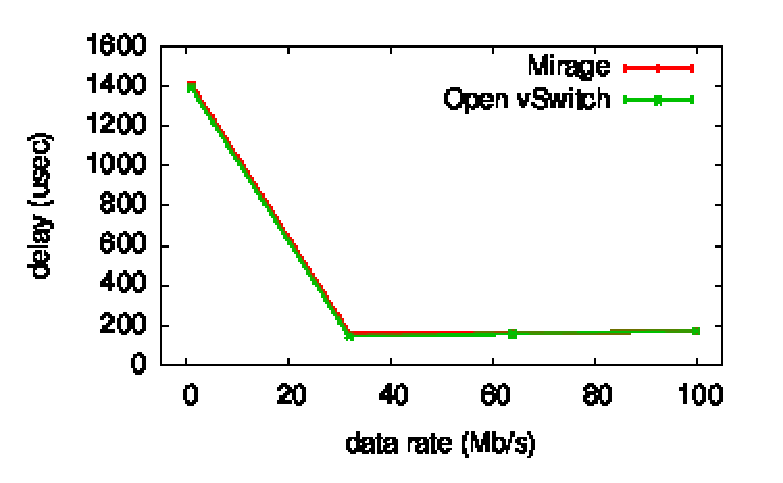
\includegraphics[width=\columnwidth]{switch-media-delay}
\caption{\label{fig:switch}Min/max/median delay switching 100\,byte packets
        when running the Mirage switch and Open vSwitch kernel module as domU
        virtual machines.}
\vspace{-2ex}
\end{figure}

Figure~\ref{fig:switch} plots as error boxes the min, median and max of the
median processing latency of ten test runs of the experiment. We can see that
the Mirage switch's forwarding performance is very close to that of Open
vSwitch, even mirroring the high per-packet processing latency with a probe
rate of 1\,Mb/s; we believe this is due to a performance artefact of the
underlying dom0 network stack. We omit packet loss due to space constraints,
but can report that both implementations suffer similar levels of packet loss.
However, the Mirage switch has a memory footprint of just 32\,MB compared with
the Open vSwitch virtual machine requirement of at least 128\,MB. We are
currently working toward better integration of the Mirage switch functionality
with the Xen network stack to achieve lower switching latency. As a result 

\subsection{NS-3 performance} \label{sec:sdnsim-ns3-perf}

In order to test the scaling properties of the NS3 backend we perform a simple
topology experiment, depicted in Figure~(Figure~\ref{Haris-Fig2}). The topology
consists of a number of switches and an even number of hosts, splitted in pairs and generating steady
state TCP between each pair. We use two variations of the topology: A
centralised topology where all hosts are  connected to a single switch, and a
localised topology, where hosts are distributed between two switches and traffic
remains local to the switch. Each switch is connected to an \of controller that
implements a learning switch. The experiment executes 30 seconds of simulation
time.

In Table~\ref{Haris-Table1}, we present the real execution time and the slowdown
factor of each simulation.  The results show that the platform can scale close
to linear when the hosts of the simulation create small autonomous partition.
In the centralised topology, the \of switch becomes a bottleneck of the simulation,
since it has to process sequentially all network events. In the localised
topology, the distributed nature of the event engine permits
parallelization of the event processing between the two switches, thus reducing
the experiment running time.

\begin{figure}
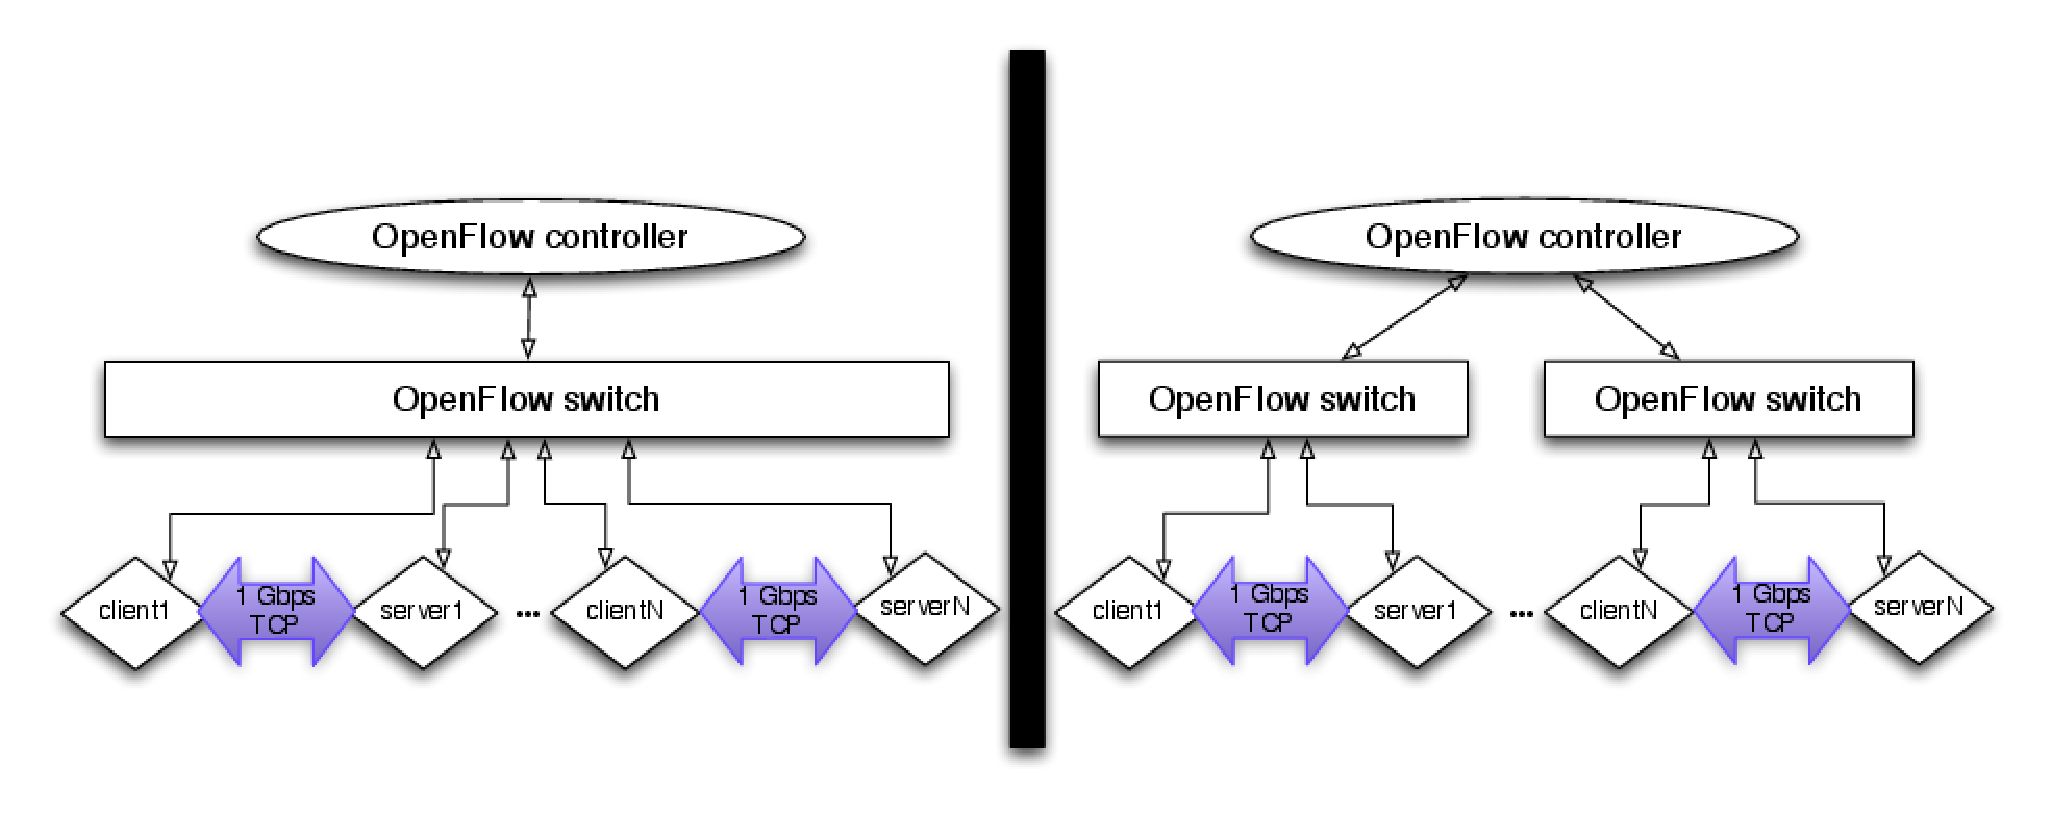
\includegraphics[width=0.9\textwidth]{sdnsim-topology}
\caption{Topology of two basic simulation scenarios for the SDNsim platform}
\label{Haris-Fig2}
\end{figure}

\begin{table}
\label{Haris-Table1}
\begin{center}
\begin{tabular}{|l|c|c|c|c|c|c|} \hline
&\multicolumn{3}{|c|}{Single Switch} & \multicolumn{3}{|c|}{two switches} \\
\cline{2-7}
Number of hosts & 2 & 8 & 12 & 4 & 8 & 12 \\
\hline 
Delay (in min) & 17 & 90 & 171 & 21 &50 & 82 \\
\hline
Slowdown factor & 34 & 180 & 242 & 42 & 100 & 164 \\
\hline 
\end{tabular}
\end{center}
\caption{\sdnsim simulation of a fat-tree topology over NS3 backend allows
  better scaling of the slowdown factor as the traffic is localised. }
\end{table}

\section{Security Tradeoffs on Datacenter Network Micro-control} \label{sec:rdsf-eval}
\todo{Maybe remove this section}
%%%%%%%%%%%%%%%%%%%%%%%%%%%%%%

\section{Summary and Conclusions}\label{sec:conclusion}
%%%%%%%%%%%%%%%%%%%%%%%%%%%%%%
\todo{Add some notes on \sdnsim}
We presented, \oflops, a tool that tests the capabilities and performance of 
OpenFlow-enabled software and hardware switches. \oflops combines advanced 
hardware instrumentation, for accuracy and performance, and provides an extensible 
software framework. We use \oflops to evaluate five different OpenFlow switch 
implementations, in terms of OpenFlow protocol support as well as performance.
%In our performance evaluation, we benchmark the packet processing, flow table
%modification and traffic statistics export functionalities of the switches.

We identify considerable variation among the tested OpenFlow implementations.
We take advantage of the ability of \oflops for data plane measurements to
quantify accurately how fast switches process and apply OpenFlow commands.
For example, we found that the barrier reply message is not correctly implemented,
making it difficult to predict when flow operations will be seen by the data plane.
Finally, we found that the monitoring capabilities of existing hardware switches 
have limitations in their ability to sustain high rates of requests. Further, at high 
rates, monitoring operations impact other OpenFlow commands.

We hope that the use of \oflops will trigger improvements in the
OpenFlow protocol as well as its implementations by various vendors.

%We also readily acknowledge this paper as a snapshot of work in
%progress; every set of results poses new questions but also the role
%of \oflops can evolve as new OpenFlow instantiations are introduced and
%existing ones refined; considerable opportunity exists for future
%work.

% LocalWords:  Oflops OpenFlow

%%% Local Variables: 
%%% mode: latex
%%% TeX-master: "../thesis"
%%% End: 

\chapter{Home network management scalability} \label{sec:homework} 

\ifpdf
\graphicspath{{Chapter2/Chapter2Figs/PNG/}{Chapter2/Chapter2Figs/PDF/}{Chapter2/Chapter2Figs/}}
\else 
\graphicspath{{Chapter2/Chapter2Figs/EPS/}{Chapter2/Chapter2Figs/}} 
\fi

In this chapter we explore applications of the SDN technology to scale network
management in home networks. Drawing conclusions from existing social and user
studies, we identify a series of user management requirements and we  
redesign the home network functionality and control abstraction addressing these
requirements. We present a Strawman implementation of a network design which
achieves simplicity and scalability of the control abstraction within the home
environment. Additionally, we propose an extension of our design, which bridges
the gap between the home network users performance requirements and the ISP
resource allocation policy, providing a simple, scalable and user-friendly QoS
mechanism.

In this chapter, motivated by the nature of the problems and the inherent
opportunities of home networks (Section~\ref{s:evolution}),  we present a home
router design~(Section~\ref{s:router}) and evaluate a number of proposed
protocol modifications placing the homeowner in direct control of their
network~(Section~\ref{s:protocols}). In addition, we present a simple QoS
mechanism enabling user-ISP collaboration to improve resource utilisation in the
last-mile bottleneck of the ISP (Section~\ref{s:qos}). Finally we conclude
the results of our exploration~(Section~\ref{s:conclusion}).

Note that throughout this Chapter we refer to the individual managing the home
network as the homeowner without loss of generality; clearly any suitably
authorised member of the household, owner or not, may be able to exercise control
based on specifics of the local context. 

\section{Motivations}\label{s:evolution}

In this section we elaborate on the nature of the problems and opportunities
inherent to home networks. We motivate motivate our thesis by presenting the
findings of relevant ethnographic and social studies
(Section~\ref{sec:homework:use_cases}) and set the requirements for our system
(Section~\ref{s:revolution}). 

\subsection{Home Network: Use cases} \label{sec:homework:use_cases}

Many empirical studies in recent years have explored the clear mismatch between
current networking technology and the needs of the domestic setting,  in both
the
UK~\mycite{tolmie07,rodden07,rodden04,rodden04,crabtree03}
and the
US~\mycite{shehan07,grinter05,sung07,chetty07,shehanpoole08}.
These studies present a weight of evidence that problems with home networking
are not amenable to solution via a `thin veneer' of user interface technology
layered atop the existing architecture.  Rather, they are \emph{structural},
emerging from the mismatch between the stable `end-to-end' nature of
the Internet and the highly dynamic and evolving nature of domestic
environments.  

Home networks use the same protocols, architectures, and tools once developed for the
Internet in the 1970s.  Inherent to the Internet's `end-to-end' architecture
is the notion that the core is simple and stable, providing only a semantically
neutral transport service.  The core protocols were designed for a certain
context of \emph{use} (assuming relatively trustworthy endpoints), made
assumptions about \emph{users} (skilled network and systems administrators both
using connected hosts and running the network core), and tried to accomplish a
set of \emph{goals} (e.g.,~scalability to millions of nodes) that simply do not
apply in a home network. 

In fact, the home network is quite different in nature to both core and
enterprise networks.  Existing studies~\mycite{tolmie07,shehan07,shehanpoole08}
suggest domestic networks tend to be relatively small in size with between 5 and
20 devices connected at a time.  The infrastructure is predominately
cooperatively self-managed by residents who are seldom expert in networking
technology and, as this is not a professional activity, rarely motivated to
become expert.  A wide range of devices connect to the home network, including
desktop PCs, games consoles, and a variety of mobile devices ranging from
smartphones to digital cameras.  Not only do these devices vary in capability,
they are often owned and controlled by different household members.  

To illustrate the situation we are addressing, consider the following three
example scenarios, drawn from  situations that emerged from fieldwork 
reported in more detail elsewhere~\mycite{wmust2011,Chetty10}: 

\begin{quote}
\textbf{Negotiating acceptable use}.  William and Mary have a spare room which
they let to a lodger, Roberto.  They are not heavy network users and so,
although they have a wireless network installed, they pay only for the lowest
tier of service and they allow Roberto to make use of it.  The lowest tier of
service comes under an acceptable use policy that applies a monthly bandwidth
cap.  Since Roberto arrived from Chile they have exceeded their monthly cap on
several occasions, causing them some inconvenience.  They presume it is
Roberto's network use causing this, but are unsure and do not want to cause
offence by accusing him without evidence.
\end{quote}

\begin{quote}
\textbf{Welcome visitors, unwelcome laptops}.  Steve visits his friends Mike and
Elisabeth for the weekend and brings his laptop and smartphone.  Mike has
installed several wireless access points throughout his home and has secured the
network using MAC address filtering in addition to WPA2.  To access the network,
Steve must not only enter the WPA2 passphrase, but must also obtain the MAC
addresses of his devices for Mike to enter on each wireless access point.  Steve
apologizes for the trouble this would cause and, rather than be a problem to his
hosts, suggests he reads his email at a local cafe.
\end{quote}

\begin{quote}
\textbf{Socially efficient network sharing}.  Richard, the teenage son of Derek
exhibits a great interest in online Music services. Derek works some times from
home, using the Terminal Services provided by his employee. Tension is created
between the household member,  as Derek blames Richard downloading activity for
his poor performing remote desktop application. 
\end{quote}

In such ways, simple domestic activities have deep implications for
infrastructures that generate prohibitive technical overheads.  In the first
scenario, the problem is simply that the network's behaviour is opaque and
difficult for normal users to inspect; in the second, the problems arise from
the need to control access to the network and the technology details exposed by
current mechanisms for doing so; in the third, the problem arises from the
inability of the resource allocation algorithm to capture the social aspect of
the home setting.  

Home networks enable provision of a wide range of services, e.g.,~file stores,
printers, shared Internet access, music distribution.  The broad range of
supported activities, often blending work and leisure, make network use very
fluid.  In turn, this makes it very hard to express explicitly \emph{a priori}
policies governing access control or resource management~\mycite{tolmie07}.
Indeed, fluidity of use is such that access control and policy may not even be
consistent, as network management is contingent on the household's immediate
needs and routines.

\subsection{Home Networks: Revolution!} \label{s:revolution}

Current network functionality is spread across multiple layers that implement
different abstractions, while multiple protocols are used to allow network hosts
to communication over these layers. Each layer exposes a different set of
control parameters and effective network management \emph{must} exercise control
on multiple layers. Ultimately, this control distribution architecture is not
scalable for the average user. Simply creating a user interface layer for the
existing network infrastructure will only reify existing problems.  Rather, we
need to investigate creation of new network architectures reflecting the
socio-technical nature of the home by taking into account both human and
technical considerations. Control of the network can be redefined, exposing only
the required control and semantically appropriate abstraction, in order to scale
controllability of the network.  
% For example, we
% may need to explore architectures that sacrifice scalability in favor of
% installability, evolvability, and maintainability.  

To this end we exploit local characteristics of the home: devices are often
collocated, are owned by family and friends who physically bring them into the
home, and both devices and infrastructure are physically accessible.
Essentially, the home's physical setting provides a significant source of
heuristics we can understand, and offers a set of well understood practises that
might be exploited in managing the infrastructure.  

We exploit human understandings of the local network and the home to guide
management of the supporting infrastructure~\mycite{crabtree03} by focusing on
the home router not only as the boundary point in an edge network but as a
physical device which can be exploited as a point of management for the domestic
infrastructure.  Within our router, we focus on flow management for three
reasons: 

\begin{itemize}
    \item we do not require forwarding scalability to the same degree as the
          core network; 
    \item doing so allows us to monitor traffic in a way that is more meaningful
          for users; and 
    \item we can apply per-flow queueing mechanisms to control bandwidth
          consumption, commonly requested by users.  
  \end{itemize}
%% \mort{distinction is now being pushed as: large-scale networks focus
%%      on packets not flows for scalability (plus other things of
%%      core/enterprise nets); we go for flows and explore impact of this
%%      decision} 

%% \mort{focusing on flows lets us (a) monitor traffic in a way that's
%%      (somewhat) meaningful for users (but cf.  wmust); (b) control
%%      traffic using a range of standard mechanisms such as per-flow
%%      queueing/qos} 

\section{Reinventing the Home Router} \label{s:router}
 
\begin{figure} 
  \centering 
  \includegraphics[trim=0.5cm 1cm 0.5cm 2.5cm, width=0.5\columnwidth]{architecture}
  \caption[Home router architecture]{\label{f:architecture}Home router architecture.  \ovs
    and NOX manage the wireless interface.  Three NOX modules
    provide a web services control API, a DHCP server with custom address
    allocation and lease management, and a DNS interceptor, all logging to the
    Homework Database (\emph{hwdb}) (\S\ref{s:protocols}). 
}\end{figure}

Our home router is based on Linux 2.6 running on a micro-PC
platform.\footnote{An Atom 1.6GHz eeePC 1000H netbook with 2GB of RAM running
  Ubuntu 10.04.} Wireless access point functionality is provided by the
\emph{hostapd} package.  The software infrastructure on which we implement our
home router, as shown in Figure~\ref{f:architecture}, consists of the \ovs \of
implementation, a NOX controller exporting a web service interface to control
custom modules that monitor and manage DHCP and DNS traffic, plus the Homework
Database~\mycite{sventek11:_infor_plane_archit_suppor_home_networ_manag} providing
an integrated network monitoring facility.  This gives us a setup very similar
to a standard operator-provided home router where a single box acts as wireless
access point, multiplexes a wired connection for upstream connectivity to the
ISP, and may provide a small number of other wired interfaces. 
                                                                    
We next describe the main software components upon which our router relies.
Using this infrastructure, a number of novel user interfaces was developed, one of
which we describe briefly below; details of the others are available
elsewhere~\mycite{mortier11:_suppor_novel_home_networ_manag}.  Note that a key
aspect of our approach is to avoid requiring installation of additional
software on client devices: doing so is infeasible in a home context where so
many different types of device remain in use over extended periods of time.

\subsection{\of, \ovs \& NOX} \label{s:openflow}

We provide \of support using \ovs~\mycite{openvswitch} and employ the
NOX~\mycite{gude08} control platform, an event-driven programmable controller with
C++ and Python module support, to develop our control logic.  Our control logic,
discussed in Section~\ref{s:protocols}, is implemented in five distinct modules.
The C++ module \textit{hwdb} synchronizes router state with the hwdb home
database, presented in Section~\ref{s:hwdb}, the C++ module
\textit{homework\_dhcp} implements our custom DHCP server, the C++ module
\textit{homework\_routing} implements the forwarding logic of the design, the
C++ module \textit{homework\_dns} implements our DNS filtering functionality and
the Python module \textit{homework\_rpc} exposes the control API through a Web
service. 

\begin{table}
  \begin{tabular} {p{0.35\columnwidth}p{0.55\columnwidth}} 
    \textbf{Method} & \textbf{Function} \\ 
    \url{permit/<eaddr>} & Permit access by specified client\\ 
    \url{deny/<eaddr>} & Deny access by specified client\\
    \url{status/[eaddr]} & Retrieve currently permitted clients, or status of specified client \\ 
    \url{dhcp-status/} & Retrieve current MAC--IP mappings\\
    \url{whitelist/<eaddr>} & Accept associations from client\\
    \url{blacklist/<eaddr>} & Deny association to client\\
    \url{blacklist-status/} & Retrieve currently blacklisted clients\\
    \url{permit-dns/<e>/<d>} & Permit access to domain \texttt{d} by client \texttt{e}\\ 
    \url{deny-dns/<e>/<d>} & Deny access to domain \texttt{d} by client \texttt{e}\\ 
  \end{tabular} 
  \caption{\label{t:api}Web service API;
    prefix all methods \texttt{https://\ldots/ws.v1/}.  $<$\,$X$\,$>$ and $[X]$
    denote required and optional parameters.}
\end{table}

Our router provides flow-level control and management of traffic via a single
\of datapath managing the wireless interface of the platform.\footnote{Without
  loss of generality, our home router has only a single wired interface so the
  only home-facing interface is its wireless interface; other home-facing
  interfaces would also become part of the \of datapath.} Control of the router
is provided via a simple web service (Table~\ref{t:api}).  Traffic destined for
the upstream connection is forwarded by the datapath for local processing via
the kernel bridge, with Linux's \emph{iptables} IP Masquerading rules providing
standard NAT functionality.\footnote{While NAT functionality could be
  implemented within NOX, it seemed neither interesting nor necessary to do so.}

%% Without loss of generality, the device we describe in this paper has
%% only a single wired interface so the only home facing interface is its
%% wireless interface, and this is the physical interface managed by the
%% OpenFlow datapath.

\subsection{The Homework Database} \label{s:hwdb}
 
%% \mort{reduce this- it's reported elsewhere: it's a streaming database,
%%  collecting ip layer supporting rpc interaction, and defaults to providing
%%  a Flows table among others; provides the basic measurement
%%  facility accessed by the many uis via rpc}
 
In addition to \ovs and NOX we make use of the Homework Database, \emph{hwdb},
an active, ephemeral stream
database~\mycite{sventek11:_infor_plane_archit_suppor_home_networ_manag}.  The
ephemeral component consists of a fixed-size memory buffer into which arriving
tuples (events) are stored and linked into tables.  The memory buffer is treated
in a circular fashion, storing the most recently received events inserted by
applications measuring some aspect of the system.  The primary ordering of
events is time of occurrence.  

The database is queried via a variant of CQL~\mycite{arasu05:_cql} able to express
both temporal and relational operations on data, allowing applications such as
our user interfaces to periodically query the ephemeral component for either raw
events or information derived from them.  Applications need not be collocated on
the router as \emph{hwdb} provides a lightweight, UDP-based RPC system that
supports one-outstanding-packet semantics for each connection, fragmentation and
reassembly of large buffers, optimization of ACKs for rapid request/response
exchanges, and maintains liveness for long-running exchanges.  Monitoring
applications request can execute temporal query on specific types of events.
\emph{hwdb} also provides notification functionality; applications may register
interest in \emph{future} behaviour patterns and receive notification when such
patterns occur in the database.  The work described in this paper makes use of
three tables: \emph{Flows}, accounting traffic to each 5-tuple flow;
\emph{Links}, monitoring link-layer performance; and \emph{Leases}, recording
mappings assigned via DHCP.

\subsection{The Guest Board} \label{s:guest-board}

% \mort{explicitly tie to ethno story} 

\begin{figure} 
  \centering 
  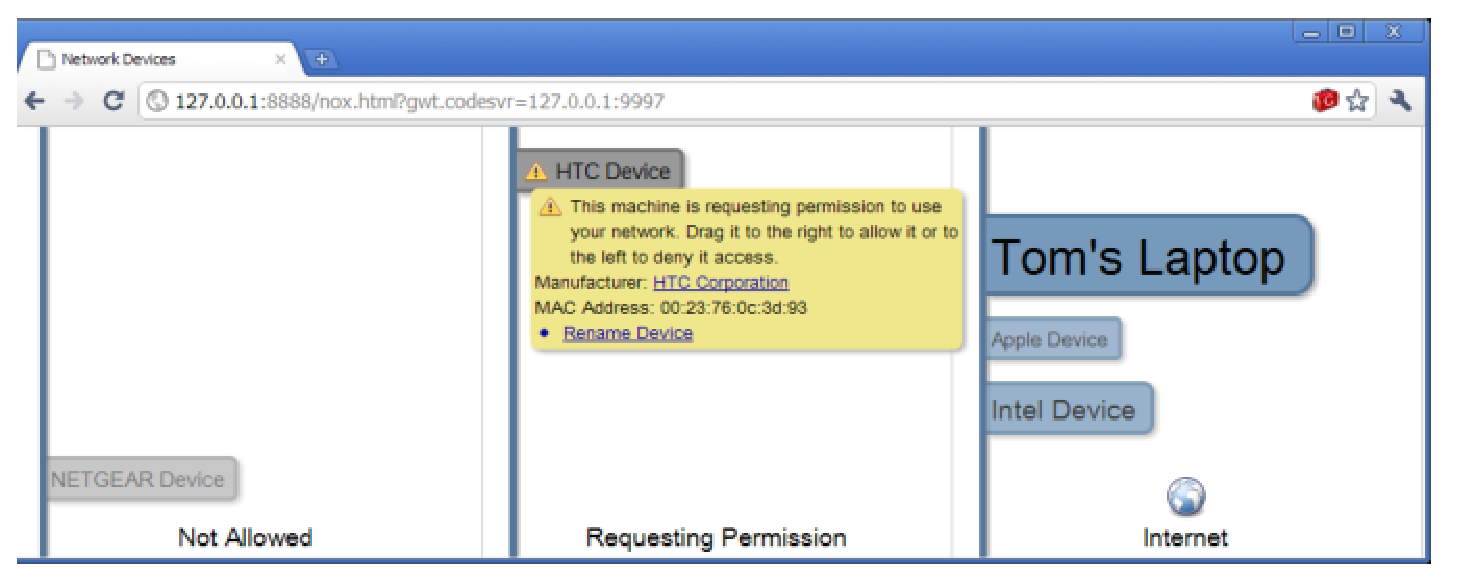
\includegraphics[width=0.9\columnwidth]{homework_guest_board}
  \caption[The \emph{Guest Board} control panel]{\label{f:guest-board}The \emph{Guest Board} control panel, showing an
    HTC device requesting connectivity.}
\end{figure}

This interface exploits people's everyday understanding of control panels in
their homes, e.g.,~heating or alarm panels, to provide users with a central
point of awareness and control for the network. This physical arrangement
provides a focal point for inhabitants to view current network status and to
manage the network.  The interface provides a real time display of the current
status of the network (Figure~\ref{f:guest-board}), showing devices in different
zones based on the state of their connectivity.  The display dynamically maps
key network characteristics of devices to features of their corresponding
labels.  Mappings in the current display are: 

\begin{itemize}
\item Wireless signal strength is mapped to device label transparency, so
      devices supplying weak signals fade into the background.
\item Device bandwidth use is proportional to its label size, e.g.,~Tom's Laptop
      in Figure~\ref{f:guest-board} is currently the dominant bandwidth user. 
\item Wireless Ethernet retransmissions show as red highlights on the device's
  label, indicating devices currently experiencing wireless reliability problems. 
\end{itemize}

Devices in range appear on the screen in real-time, initially in the leftmost
panel indicating they are within range of the home router but not connected.
The central panel in the control displays machines actively seeking to associate
to the access point. This zone exploits the underlying strategy of placing
people in the protocol, discussed in Section~\ref{s:protocols}.  When devices
unknown to the network issue DHCP requests, the router's DHCP server informs the
guest board and a corresponding label appears in this portion of the display.
If a user wishes to give permission for the machine to join the network they
drag the label to the right panel; to deny access, they drag the label to the
left panel. The guest board provides both a central control point and, by
drawing directly upon network information collected within our router, a
network-centric view of the infrastructure. 

\section{Putting People in the Protocol} \label{s:protocols}

%\mort{note that this is tied to social convention of home visiting, network
%part of the home not separate to it, etc}
We use our home router to enable \emph{ad hoc} control of network policy by
non-expert users via interfaces such as the Guest Board
(Figure~\ref{f:guest-board}).  This sort of control mechanism is a natural fit
to the local negotiation over network access and use that takes place in most
home contexts.  While we believe that this approach may be applicable to other
protocols, e.g.,~NFS/SMB, LPD, in this section we demonstrate this approach via
our implementation of a custom DHCP server and selective filters for wireless
association and DNS that enable management of device connectivity on a
per-device basis. 

Specifically, we describe and evaluate how our router manages IP address
allocation via DHCP, two protocol-specific (EAPOL and DNS) interventions it
makes to provide finer-grained control over network use, and its forwarding
path.  We consider three primary axes: \emph{heterogeneity} (does it still
support a sufficiently rich mix of devices); \emph{performance} (what is the
impact on forwarding latency and throughput of our design and implementation
decisions); and \emph{scalability} (how many devices and flows can our router
handle).  In general we find that our home router has ample capacity to support
observed traffic mixes, and shows every indication of being able to scale beyond
the home context to other situations, e.g., small offices, hotels. 

\subsection{Address Management} \label{s:addresses}

DHCP~\mycite{rfc:2131} is a protocol that enables automatic host network
configuration. It is based on a four way broadcast handshake that allows hosts
to discover and negotiate with a server their connectivity parameters.  As part
of our design we extend the functionality of the protocol to achieve two goals.
First, we enable the homeowner to control which devices are permitted to connect
to the home network by interjecting in the protocol exchange on a case-by-case
basis.  We achieve this by manipulating the lease expiry time, allocating only a
short lease (30s) until the homeowner has permitted the device to connect via a
suitable user interface.  The short leases ensure that clients will keep
retrying until a decision is made; once a device is permitted to connect, we
allocate a standard duration lease (1 hour).

Second, we ensure that all network traffic is visible to the home router and
thus can be managed through the various user interfaces built against it.  We do
so by allocating each device to its own /30 IP subnet, forcing inter-device
traffic to be IP routed via our home router.  This requirement arises because
wireless Ethernet is a broadcast medium so clients will ARP for destinations on
the same IP subnet enabling direct communication at the link-layer.  In such
situations, the router becomes a link-layer device that simply schedules the
medium and manages link-layer security -- some wireless interfaces do not even
make switched Ethernet frames available to the operating system. The result
is that traffic between devices in the
home, such as music distribution and file stores, becomes invisible to the
home router.  By allocating addresses from distinct subnets, all traffic
between clients must be transmitted to the gateway address, ensuring all
traffic remains visible to our home router. 
Our custom DHCP server allocates /30 subnet to each host from 10.2.*.*/16 with
standard address allocation within the /30 (i.e.,~considering the host part of
the subnet, 00 maps to the network, 11 maps to subnet broadcast, 01 maps to the
gateway and 10 maps to the client's interface itself). Thus, each local device
needs to route traffic to any other local device thought the router, making
traffic visible in the IP layer.
%% We deal with the case of
%% misbehaving/malicious clients attempting to subvert our address
%% allocations in~\S\ref{s:association}. 
% \mort{point to lack of perf implications?  or just pull to here?}
%
% The DHCPOFFER generated by our home router in response to a previously unknown
% client allocates a /30 subnet from 10.2.*.*/16 with standard address
% allocation within the /30 (i.e.,~considering the two least significant bits of
% the subnet, 00 maps to the network, 11 maps to subnet directed broadcast, 01
% maps to the gateway and 10 maps to the client's interface itself).  This
% allocation pattern ensures that all traffic for locally connected devices is
% sent via the router, since all devices are on distinct, non-overlapping IP
% subnets.  This would not be the case if addresses were allocated to clients
% from the same subnet, e.g.,~clients were all simply allocated addresses
% directly from 10.*.*.*/8.

We measured the performance of our DHCP implementation and found that, as
expected, per-request service latency scales linearly with the number of
simultaneous requests.  Testing in a fairly extreme scenario, simultaneous
arrival of 10 people each with 10 devices,  gives a median per-host service time
of 0.7s.

\subsection{Per-Protocol Intervention} \label{s:association}

Our current platform intervenes in two specific protocols providing greater
control over access to the wireless network itself, and to Internet services
more generally. 

\begin{figure} \centering \includegraphics[width=0.8\columnwidth]{eapol}
  \caption[802.11i handshake]{\label{f:association}802.11i handshake, part of the association
    process.  Note that MIC (Message Integrity Code) is an alternate term for
    MAC, used in such contexts to avoid confusion with Media Access Control.}
  \end{figure}
 
%% \mort{also intercept DNS- figures from previous section show that this
%%      will introduce negligible extra latency} 

Our home router supports wireless Ethernet security via 802.11i with EAP-WPA2,
depicted in Figure~\ref{f:association}, using \emph{hostapd}.  In EAP-WPA2
security mechanism, the
client (\emph{supplicant}) and our router (\emph{authenticator}) negotiate two
keys derived from the shared master key via a four-way handshake, through the
EAPOL protocol.  The \emph{Pairwise Transient Key} (PTK) is used to secure and
authenticate communication between the client and the router; the \emph{Group
  Transient Key} (GTK) is used by the router to broadcast/multicast traffic to
all associated clients, and by the clients to decrypt that traffic.  All
non-broadcast communication between clients must therefore pass via the router
at the link-layer (for decryption with the source's PTK and re-encryption with
the destination's PTK), although the IP routing layers are oblivious to this if
the two clients are on the same IP subnet.\footnote{The 802.11i specification
  defines a general procedure whereby two clients negotiate a key for mutual
  communication (\emph{Station-to-station Transient Key}, STK).  However, the
  only use of this procedure in the specification is in \emph{Direct Link Setup}
  (DLS) used in supporting 802.11e, quality-of-service.  This can easily be
  blocked by the access point, and in fact is not implemented in the
  \emph{hostapd} code we use, so we do not consider it further.
  %\mort{emphasise this bit?  also wifidirect - embedding of ``soft'' ap inside
  %wifi device - completely orthogonal?}i
  }

Periodically, a timeout event at the access point initiates rekeying of the PTK,
visible to clients only as a momentary drop in performance rather than the
interface itself going down.  We use this to apply blacklisting of clients
deemed malicious, such as a client that attempts to communicate directly (at the
link-layer) with another client, i.e.,~attempting to avoid their traffic being visible
to our home router.  We wait until the rekeying process begins and then decline
to install the appropriate rule to allow rekeying to complete for the client in
question.  This denies the client access even to link-layer connectivity, as
they will simply revert to performing the four-way handshake required to obtain
the PTK\@.  This gives rise to a clear trade-off between security and performance:
the shorter the rekeying interval, the quicker we can evict a malicious client
but the greater the performance impact on compliant clients.  

\begin{figure} 
  \centering 
  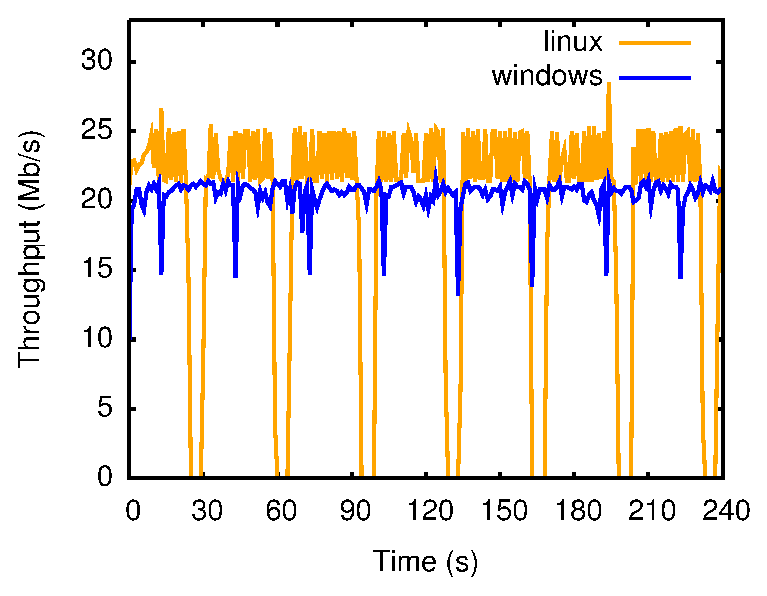
\includegraphics[width=0.5\columnwidth]{Chapter2/Chapter2Figs/rekeying}
  \caption[Affect on TCP throughput from 802.11i rekeying]
  {\label{f:rekeying}Affect on TCP throughput from 802.11i rekeying every 30s
      for Linux 2.6.35 using a Broadcom card with the \emph{athk9} module; and
      Windows 7 using a proprietary Intel driver and card.} 
\end{figure}

\begin{figure*} \centering
 \subfigure[homework switching latency up to 10k concurrent flows]{\includegraphics[width=0.45\columnwidth]{Chapter2/Chapter2Figs/latency-test}\label{f:homework:performance-latency-small}}
 \subfigure[homework packet throughput up to 10k concurrent flows]{\includegraphics[width=0.45\columnwidth]{Chapter2/Chapter2Figs/throughput-test}\label{f:homework:performance-throughput-small}}
 \subfigure[homework switching latency up to 50k concurrent flows]{\includegraphics[width=0.45\columnwidth]{Chapter2/Chapter2Figs/latency-large-test}\label{f:homework:performance-latency}}
 \subfigure[homework packet throughput up to 50k concurrent flows]{\includegraphics[width=0.45\columnwidth]{Chapter2/Chapter2Figs/throughput-large-test}\label{f:homework:performance-throughput}} 
 \caption[Switching performance of home router]{\label{f:performance}Switching performance of \ovs component
    of our home router showing increasing median per-packet latency
    (Figure~\ref{f:homework:performance-latency},~\ref{f:homework:performance-latency-small}) and
    decreasing median packet throughput
    (Figure~\ref{f:homework:performance-throughput},~\ref{f:homework:performance-throughput-small}) with the number of flows.  The upper set
    of graphs
    (Figure~\ref{f:homework:performance-throughput},\ref{f:homework:performance-latency}) extends the $x$-axis from 10,000 to 500,000.}
\end{figure*}

To quantify the impact of 802.11i rekeying, we observed throughput over several
rekeying intervals.  Figure~\ref{f:rekeying} shows the transient impact to a
steady-state TCP flow of setting the
rekeying interval to 30s: rekeying causes a periodic dip in throughput as the
wireless Ethernet transparently buffers packets during rekeying before
transmitting them as if nothing had happened.  This shows the trade-off between
performance and responsiveness of this approach: to be highly responsive in
detection of misbehaving clients imposes a small performance degradation.  As a
compromise, when a device is blacklisted, all of its traffic and subsequent
rekeying exchanges are blocked.  Thus the misbehaving device is prevented from
sending or directly receiving any traffic before rekeying takes place, The
device will be able to receive only broadcast traffic in the interim due, to the
use of the GTK for such frames, until the AP initiate the negotiation of a new
key.  This allows us to pick a relatively long rekey interval (5 minutes) while
still being able to respond quickly to misbehaving devices.

We also intercept DNS to give fine-grained control over access to Internet
services and websites.  DNS requests are intercepted and dropped if the
requesting device is not permitted to access that domain.  Any traffic the
router encounters that is not already permitted by an explicit OpenFlow flow
entry has a reverse lookup performed on its destination address.  If the
resulting name is from a domain that the source device is not permitted to
access, then a rule will be installed to drop related traffic.  Performance is
quite acceptable, as indicated by latency results in Figure~\ref{f:performance}:
the extra latency overhead introduced by our router is negligible compared to
the inherent latency of a lookup to a remote name server.  
% Extending this
% fine-grained control requires more accurate identification of traffic to
% application, particularly for more complex network uses such as BitTorrent and
% Skype, and is a problem we are investigating in ongoing work.

\subsection{Forwarding} \label{s:forwarding}
 
Our router consists of a single \ovs that manages interface
\emph{wlan0}.  \ovs is initialised with a set of flows that push
DHCP/BOOTP and IGMP traffic to the controller for processing.
\ovs by default will also forward to the controller traffic not matched
by any other installed flow, which is handled as follows:

\textbf{Non-IP traffic}.  The controller acts as a proxy ARP server, responding
to ARP requests from clients.  Misbehaving devices are blacklisted via a rule
that drops their EAPOL~\mycite{rfc:3748} traffic thus preventing session keys
negotiation.
% implementing the WPA security association with the access point, so dropping
% it, prevents association.  
Finally, other non-IP non-broadcast traffic has source and destination MAC addresses verified
to ensure both are currently permitted.  If so, the packet is forwarded up the
stack if destined for the router, or to the destination otherwise.  In either
case, a suitable \of rule with a 30 second idle timeout is also installed to
shortcut future matching traffic.

\textbf{Unicast IP traffic}.  First, a unicast packet is dropped if it does not
pass all the following tests: 
\begin{itemize}
    \item its source MAC address is permitted; 
    \item its source IP address is in 10.2.x.y/16; and
    \item its source IP address matches that allocated by DHCP\@.  For valid
      traffic destined to the Internet, a flow is inserted that forwards packets
      upstream via the bridge and IP masquerading.  
\end{itemize} 
Unicast IP traffic that passes but is destined outside the home network has a
rule installed to forward it upstream via the bridge and IP masquerading.  For
traffic that is to remain within the home network a flow is installed to route
traffic as an IP router, i.e.~rewriting source and destination MAC addresses
appropriately.  All these rules are installed with 30s idle timeouts, ensuring
that they are garbage collected if the flow goes idle for over 30s.

\textbf{Broadcast and multicast IP traffic}.  Due to our address allocation
policy, broadcast and multicast IP traffic requires special attention.  Clients
send such traffic with the Ethernet broadcast bit\footnote{I.e.,~the most
  significant bit of the destination address} set, normally causing the hardware
to encrypt with the GTK rather than the PTK so all associated devices can
receive and decrypt those frames directly.  In our case, if the destination IP
address is all-hosts broadcast, i.e.,~255.255.255.255, the receiver will process
the packet as normal.  Similarly, if the destination IP address is an IP
multicast address, i.e.,~drawn from 224.*.*.*/4, any host subscribed to that
multicast group will receive and process the packet as normal. Finally, for
local subnet broadcast the router will rebroadcast the packet, rewriting the
destination IP address to 255.255.255.255. This action is required because the
network stack of the hosts filters broadcast packets from different IP subnets.

To assess switching performance, we examine both latency and packet throughput
as we increase the number of flows, $N$, from 1--500,000. In this measurement we
employ a PC, functioning as a data generator and receiver, connected directly
over a 1~Gbps full-duplex Ethernet link to our home route configured to forward all
received packets back to the incoming port. 
% During the experiment, the
% measurement PC uses the pktgen~\mycite{pktgen} kernel module to generate 1 Gbps 
% UDP traffic from a single IP address targeting variable
% number of destination hosts, thus introducing an equivalent number of network
% flows in the network, and measures the processing delay of the router, to
% receive a packet on a port and forward it back the same port. 
Each test runs for two minutes, a sufficient period to oberve the network
performance behaviour, generating packets at line rate from a single
source to $N$ destinations each in its own 10.2.*.*/30 subnet, creating equally
$N$ unique network flows.  As these are stress tests we use large packets
(1500B) for the latency tests and minimal packets (70B)\footnote{The 30B extra
  overhead is due to \emph{pktgen}~\mycite{olsson05}, the
  traffic generation tool used.} for the throughput tests, selecting
destinations at random on a per-packet basis.  Results are presented as the
median of 5 independent runs with error bars giving the min and max values. 

Figure~\ref{f:performance} shows median per-packet switching delay and per-flow
packet throughput using either exact-match rules or a single wildcard rule per
host.  Performance is quite acceptable with a maximum switching delay of
560$\mu$s and minimum throughput of 40,000
packets/second~(Figure~\ref{f:homework:performance-latency},\ref{f:homework:performance-latency-small});
initial deployment data suggests a working maximum of 3000 installed flows which
would give around 160,000 packets/second throughput (small packets) and
500$\mu$s switching delay (large
packets)~(Figure~\ref{f:homework:performance-latency-small},\ref{f:homework:performance-throughput-small}).
Using a similar topology we evaluate the performance of multi-homing in Linux hosts.
Figure~\ref{f:stack-throughput} shows that the Linux
networking stack is quite capable of handling the unusual address allocation
pattern resulting from the allocation of each wireless-connected device to a
distinct subnet which requires the router's wireless interface to support an IP
address per connected device. Increasing the number of assigned IP address has
no impact on the processing latency and minimizes marginally the maximum packet
processing rate. This performance behaviour can also be explained by the trie
data structure, used by thr Linux kernel to implement longest prefix match, which scale
lookup complexity logarithmically with respect to the number of IP addresses. 

\subsection{Discussion}

Our evaluation shows that \ovs can handle orders of magnitude more rules
than required by any reasonable home deployment.  Nonetheless, to protect
against possible denial-of-service attacks on the flow tables, whether
accidental or malicious, our home router monitors the number of
per-flow rules introduced for each host.  If this exceeds a threshold then
the host has its per-flow rules replaced with a single per-host rule, while the
router simultaneously invokes user interface callback to inform the homeowner of the
device's odd behaviour. 

The final aspect to our evaluation is compatibility: given that our router
exercises protocols in somewhat unorthodox ways, how compatible is it with
standard devices and other protocols?  We consider compatibility along three
separate dimensions: range of existing client devices; deployed protocols that
rely on broadcast/multicast behaviours; and support for IPv6. 

\begin{figure} 
  \centering 
  \subfigure[Packet
  throughput]{\includegraphics[width=0.49\columnwidth]{Chapter2/Chapter2Figs/stack-throughput-latency}\label{f:homework:stack-throughput}}
  \subfigure[Packet
  latency]{\includegraphics[width=0.49\columnwidth]{Chapter2/Chapter2Figs/stack-throughput-throughput}\label{f:homework:stack-latency}}
  \caption[Switching performance of Linux network]{\label{f:stack-throughput}Switching performance of Linux network
    stack under our address allocation policy. Throughput
    (Figure~\ref{f:homework:stack-throughput}) shows a
    small linear decrease while switching delay
    (Figure~\ref{f:homework:stack-latency}) remains
    approximately constant as the number of addresses allocated to the interface
    increases.} \end{figure}

\paragraph{Devices} Although we exercise DHCP, DNS and EAPOL in unorthodox ways
to control network access, behaviour follows the standards once a device is
permitted access.  To verify that our home router is indeed suitable for use in
the home, we tested against a range of commercial wireless devices running a
selection of operating systems. 

\begin{table*} \centering\footnotesize
  \begin{tabular}{lp{0.33\textwidth}p{0.42\textwidth}} \bf Device & \bf Denied &
    \bf Blacklisted\\

Android 2.x & Reports pages unavailable due to DNS.  & Retries several times
before backing off to the 3g data network.\\

iTouch/iPhone & Reports server not responding after delay based on configured
DNS resolver timeout.  & Requests new wireless password after 1--2 minutes.\\

OSX 10.6 & Reports page not found based on configured DNS resolver timeout.  &
Requests new wireless password after 1--2 minutes.\\

Microsoft Windows XP & Silently fails due to DNS failure.  & Silently
disconnects from network after 4--5 minutes.\\

Microsoft Windows 7 & Warns of partial connectivity.  & Silently disconnects
from network after 4--5 minutes.\\

Logitech Squeezebox & Reports unable to connect; allows server selection once
permitted.  & Flashes connection icon every minute as it attempts and fails to
reconnect.  \\ 

Nintendo Wii & Reports unable to reach server during ``test'' phase of
connection.  & Reports a network problem within 30s.\\

Nokia Symbian OS & Reports ``can't access gateway'' on web access.  & Reports
disconnected on first web access.\\ \end{tabular}
\caption{\label{t:devices}Observed interactions between devices and our home
  router when attempting to access the network.}
\end{table*}

Table~\ref{t:devices} shows the observed behaviour of a number of common
home-networked devices: in short, all devices operated as expected once
permitted access.  DNS interception was not explicitly tested since, as an
inherently unreliable protocol, all networking stacks must handle the case that
a lookup fails anyway.  Most devices behaved acceptably when denied access via
DHCP or EAPOL, although some user interface improvements could be made if the
device were aware of the registration process.  The social context of the home
network means no problem was serious: in practice the user requesting access
would be able to interact with the homeowner, enabling social negotiation to
override any user interface confusion. 

%% We initially investigated using different subnet allocations with
%% short (30s) lease times to more easily distinguish hosts that are
%% trying to connect but are waiting for the homeowner to permit them
%% access.  Unfortunately, due to a variety of issues with common client
%% DHCP implementations, e.g., Android not correctly obeying lease
%% times,\footnote{\url{http://www.net.princeton.edu/android/android-stops-renewing-lease-keeps-using-IP-address-11236.html}} 
%% this broke device interfaces sufficiently that doing so would only
%% increase user confusion.

\paragraph{Broadcast protocols} A widely deployed set of protocols relying on
broadcast and multicast behaviours are those for `zero conf' functionality.  The
most popular are Apple's \emph{Bonjour} protocol; \emph{Avahi}, a Linux variant
of Bonjour; Microsoft's \emph{SSDP} protocol, now adopted by the UPnP forum; and
Microsoft's \emph{NetBIOS}.  

Bonjour and Avahi both rely on periodic transmission of multicast DNS replies
advertising device capabilities via TXT records.  SSDP is similar, but built
around multicast HTTP requests and responses.  We tested Bonjour specifically by
setting up a Linux server using a Bonjour-enabled daemon to share files.  We
observed no problems with any clients discovering and accessing the server, so
we conclude that Bonjour, Avahi and SSDP would all function as expected. 

NetBIOS is somewhat different, using periodic network broadcasts to disseminate
hosts' capabilities.  In doing so we observed a known deficiency of NetBIOS: it
cannot propagate information for a given workgroup between different
subnets.\footnote{\url{http://technet.microsoft.com/en-gb/library/bb726989.aspx}}
However, installing a WINS server on the router mitigates this problem.
%\mort{although ugly, this would work at little cost and the other benefits seem
%significant. no extra attack surface because can configure nox/ovs/firewall to
%deny access to it from outside the home network}

In general, it may seem that our address allocation policy introduces link-layer
overhead by forcing all packets to be transmitted twice in sending them via the
router.  However this is not the case: due to use of 802.11i, unicast IP traffic
between two local hosts must \emph{already} be sent via the access point.  As
the source encrypts its frames with its PTK, the access point must decrypt and
re-encrypt these frames with the destination's PTK in order that the destination
can receive them.  Multicast and all-hosts broadcast IP traffic is sent using
the GTK, so can be received directly by all local hosts.  Only directed
broadcast IP traffic incurs overhead which though is a small proportion of the
total traffic; data from a limited initial deployment (about one month in two
homes) suggests that broadcast and multicast traffic combined accounts for less
that 0.1\% (packets and bytes) in both homes.
% \mort{cite?}
%, concurring with other larger (albeit non-domestic) datasets.  we have already
%discussed this previsouly : although other clients receive it at the
%link-layer, the address allocation policy means they will discard it, leaving
%it to the home router to replicate and retransmit all such traffic.  We do not
%consider this significant as data from a limited initial deployment (about one
%month in two homes) suggests that a very small amount of traffic is affected:
%broadcast and multicast traffic combined accounts for less that 0.1\% (packets
%and bytes) in both homes, concurring with other larger (albeit non-domestic)
%datasets.\mort{cite?}


\paragraph{IPv6 support} 

IPv6 support is once more receiving attention due to recent exhaustion of the
IPv4 address space.  Although our current implementation does not support IPv6
due to limitations in the current Open vSwitch and NOX releases,\footnote{\of
  provides support in its 1.4 release of the protocol; NOX currently has no
  support for IPv6; and \ovs only supports IPv6 as a vendor extension of the
  OpenFlow protocol.} we briefly discuss how IPv6 would be supported on our
platform.  While these limitations prevent a full working implementation in our
platform, we have verified that behaviour of both DHCPv6 and the required ICMPv6
messages was as expected, so we do not believe there are any inherent problems
in the approaches we describe below.

Addition of IPv6 support affects the network layer only, requiring consideration
of routing, translation between network and link layers, and address
allocation.  Deployment of IPv6 has minimal impact on routing, limited to the
need to support 128~bit addresses and removal, in many cases, of the need to
perform NAT~\footnote{Some operators may still prefer to use NAT as part of a
  legacy of address management and operations.}.  Similarly, supporting
translation to lower layer addresses equates to supporting ICMPv6 Neighbour
Solicitation messages which perform equivalent function to ARP.

Address allocation is slightly more complex but still straightforward.  IPv6
provides two address allocation mechanisms: \emph{stateless} and
\emph{stateful}.  The first allows a host to negotiate directly with the router
using ICMPv6 Router Solicitation and Advertisement packets to obtain network
details, IP netmask and MAC address.  Unfortunately this process requires that
the router advertises a 64 bit netmask, of which current plans allocate only one
per household, with the result that all hosts would end up on the same subnet.
The second builds on DHCPv6 where addresses are allocated from a central entity
and may have arbitrary prefix length.  This would enable our router to function
in much the same manner as currently, although it would need to support the
ICMPv6 Router Advertisement message to support router discoverability by hosts. 

In order to test the functionality, we set up a simple hardcoded version of our
design. Specifically, we allocate a public IPv6 /64 prefix to our home router.
The router uses the ISC DHCPv6 server implementation, configured to allocate
addresses from a /120 subnet.  Additionally, on the router we run the RADVD
daemon to reply appropriately to ICMPv6 messages.  Using this network setup, we
tested MacOSX, Windows and Linux IPv6 network stacks and verified correct network
configuration and Internet connectivity. 


\section{Putting people in the Resource Allocation Policy}\label{s:qos}

\begin{figure}
  \centering
  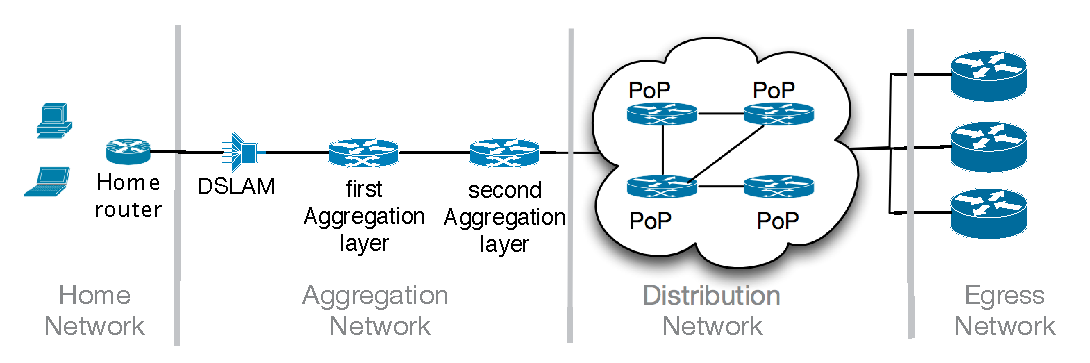
\includegraphics[width=0.95\columnwidth]{isp_plan}
  \caption[ISP network architecture]{\label{fig:isp_plan} ISP network architecture is logically divided in 3
    zones: The {\it Aggregation Network}, the {\it Distribution Network}\/ and
    the {\it Egress Network}.}
\end{figure}

As we have discussed in Section~\ref{sec:intro:net_evolution}, providing strong
performance guarantees in large production networks using commodity technologies
exhibits poor scalability. There are two primary approaches followed by the network
community, to scale resource allocation policies: \emph{network resource
  over-provision}; and \emph{application-aware traffic engineering}.  Resource
over-provision increases available resources thus removing performance
bottlenecks. Application-aware network engineering extends the network
policy to  manage efficiently application traffic, e.g.~VoIP traffic is serviced
by a separate high-priority VLAN\@. Nonetheless, the applicability of these
approaches in broadband networks is limited. On the one hand, resource
over-provision faces a non-scalable deployment cost on the edges of the
network~\footnote{Optical link installation costs vary between \$50-\$200 per
  foot, while fiber installation in municipal areas has an annual cost of \$1.91
  per foot~\mycite{backhaul-cost}. Such upgrades preclude a significant upgrade
  cost for equipment.}, while, on the other hand, application-aware network
engineering raises legal issues for Internet providers~\mycite{hahn06}. In this
section, we propose an architectural extension in the last-mile of the ISP,
enabling homeowners to define per-application resource requirements.  The
architecture improves the ISP resource allocation policy, as well as, the user
experience.  For the rest of this section, we discuss the architecture of
current broadband networks and their  inherent limitations in resource allocation
(Section~\ref{s:qos:motivation}), we present the architecture of our
system (Section~\ref{s:qos:architecture}), and we evaluate its impact on specific
applications classes (Section~\ref{s:qos:eval}).

\subsection{ISP resource allocation} \label{s:qos:motivation}

In order to motivate the reader on the benefits of our architecture, we firstly
present the architecture of current broadband networks and identify their
performance bottleneck. Figure~\ref{fig:isp_plan} presents a generic model for
the network architecture for a residential broadband ISP\@. Although, exact
architecture details remain undisclosed, there is a high level design pattern,
organising the ISP network in three domains: the \textit{aggregation network};
the \textit{distribution network}; and the \textit{egress network}. The
aggregation network contains the digital subscriber line access multiplexer
(DSLAM) which translates DSL packets to Ethernet frames, the Broadband Remote
Access Server (BRAS), an authenticating and policy enforcing network device,
and a series of aggregation switches which multiplex traffic between the BRAS and
the distribution network.  Traffic from the aggregation network routes through
the distribution network towards either the egress network or towards a local
aggregation switch. The distribution network consists of a small number of
large routers interconnected using high capacity links.  ISPs typically employ
network tunnelling technologies, like MPLS, in the distribution network to
minimize forwarding state.  The egress network of an ISP consists of large
routers, hosted in Internet Exchange Points (IXP), which connect the ISP with
peering ASes.

A number of research papers have identified a significant bottleneck in the
last-mile of the network~\mycite{Dischinger:2007bg,Akella2003}: the link between
the DSLAM and the aggregation network. This bottleneck can be explained by the
high oversubscription ratio of such links, which commonly varies between 10:1
and 50:1~\mycite{canada-subscription}, depending on population density of an area
and market dynamics~\mycite{sky-oversubscription}.  

Our system aims to bridge a fundamental communication gap between the ISP and
homeowners. Users perceive network traffic as an ensemble of flows belonging to
a specific application and priority class within the home social context,
e.g.~Skype VoIP traffic has a higher priority than web browsing traffic and
parents' teleworking traffic is more important than kids' entertainment traffic.
ISPs view household traffic as a packet aggregate with a specific IP address, on
which resource allocation mechanisms apply monthly or daily traffic
caps~\mycite{virgin-caps,bt-caps}.  Network caps rate-limit heavy-hitting
households and provide long-term fairness between users. This approach degrades
severely the short-term performance for latency-bound applications, such as
remote desktop and VoIP\@. Effectively, there is an incentive for ISPs and
homeowners to collaborate and control more efficiently the traffic resources
within the user cap.  Homeowners can annotate high priority flows within their
traffic aggregate and thus improve their experience. ISPs can increase
the user-friendliness of their network policy and offload some of the resource
allocation complexity to end-users. 

Our design virtualises network control and resources in the last-mile and
delegates control to a homeowner-managed \of controller.  The household
controller uses the \of protocol to assign traffic flows to appropriate priority
queues.  While the proposed solution cannot always guarantee end-to-end resource
allocation, it provides a sufficient mechanism to handle in a user-friendly
manner edge-network congestion, and scale the configuration complexity. 

\subsection{Architecture Design} \label{s:qos:architecture}

Congestion in the last-mile requires resource control both in the home network
and within the ISP network. Home traffic is asymmetric and  the network
bottleneck lies beyond the control of the homeowner, thus requiring control on
both traffic directions.  Our architecture consists of three subsystems: a
data-collection daemon on the end-systems of the home network, a FlowVisor
instance in the ISP network translating user flow prioritisation into
forwarding policy, and a policy enforcing daemon on the home network router. 

\paragraph*{Data collection on End-systems}

In order to map network flows to applications, we developed a light cross-platform
daemon recording the content of the end-host connection table.  The daemon
collects mappings between flow tuples and applications names.  Information is
collected from the connection table of the OS and stored in the HWDB database.
The daemon accesses the connection table entries using the
\textit{netfilter-conntrack} library~\mycite{netfilter} in Linux systems, the
\textit{Windows Filtering Platform}~\mycite{win-wfp} in Windows systems and the
\textit{sysctl} for Darwin/MacOSX system.  In order to match each network tuple
with an application, we use the \texttt{lsof} command in Unix-like systems and
the \texttt{netstat -p} command in Windows.


\paragraph*{ISP policy translation}

\begin{figure}
  \centering
  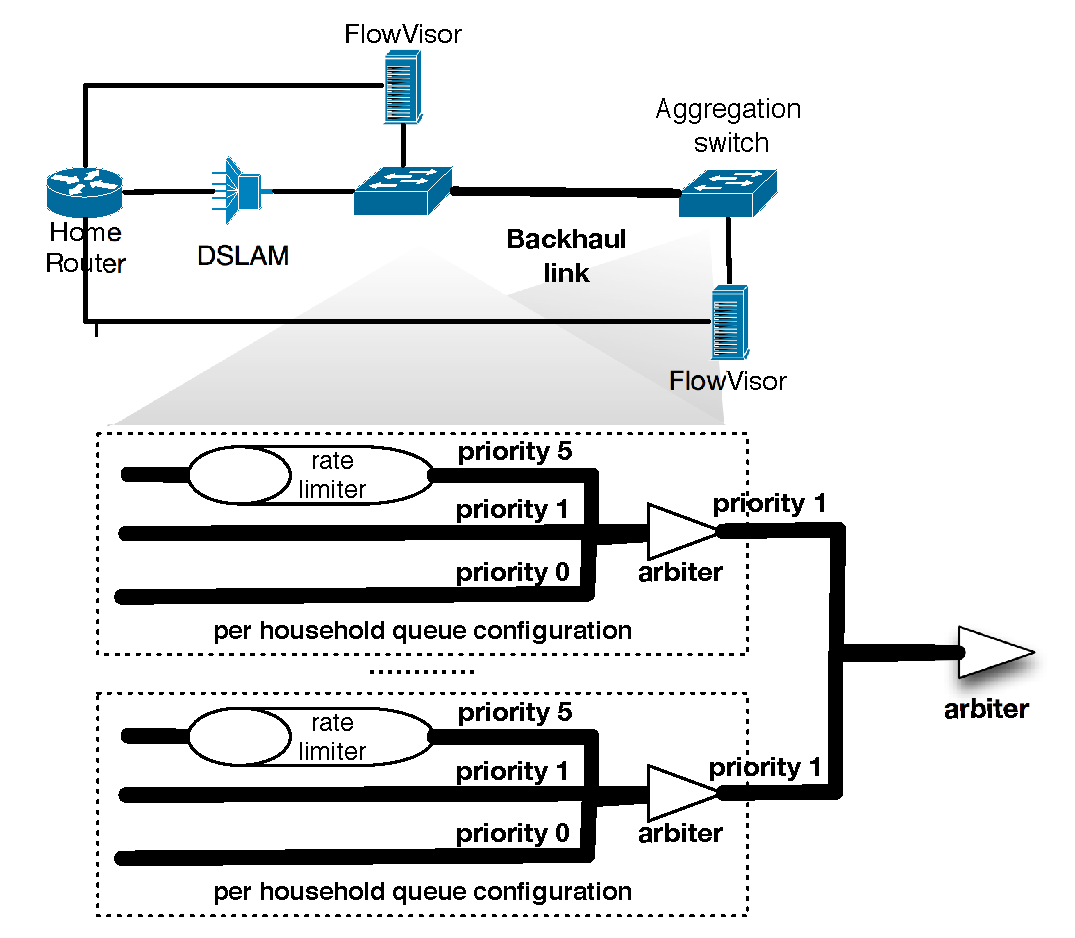
\includegraphics[width=0.7\columnwidth]{queue_design}
  \caption[User-driven QoS architecture]{User-driven network resource allocation architecture. 
    \label{fig:queue_design} A virtual control slice of the downlink between the backhaul
    network and the DSLAM is exposed to each homeowner.  The switch
    uses three queues per-household: A {\it low latency,
      high priority} \/queue, a {\it medium priority} \/queue and a {\it default}
    \/queue.}
\end{figure}

Figure~\ref{fig:queue_design} presents the network architecture of our system.
The resource mechanism exercises control on the home router and on the first layer
of aggregation switches.  The ISP exposes an \of control abstraction which
virtualises switch resources on the aggregation switches using
FlowVisor~\mycite{flowvisor-osdi}, while each home router runs an \of
controller, controlling the home Internet traffic.  The FlowVisor is configured
to provide a clean separation between household control domains in order to
mitigate control or eavesdropping attacks between households. \texttt{pkt\_in}
messages are propagated only to the respective home controller based on IP
addresses, and the home controller can only view and insert flows containing
public IP of the home network\@.   In the household, the resource control mechanism
augments the control logic, presented in the previous section. In order to
minimize forwarding state in the ISP network, the control abstraction on the
aggregation switches is used to control only the incoming Internet traffic,
while the outgoing traffic can be effectively controlled on the local router. 

At the aggregation switch and the home router, we setup three traffic shaping
queues for each household. A \textit{low latency, high priority}~(LLHP) queue, a
\textit{medium priority}~(MP) queue and a default queue.  The LLHP queue has the
highest priority between the household queues and rate limits traffic to the
minimum guaranteed bandwidth per-household~(e.g.~for 1GbE uplink with a sharing
ratio of 1:100, the LLHP queue will limit traffic to 10Mbps), providing strong
low-bandwidth and low-latency guarantees. The MP queue doesn't enforce any rate
limit, but it has a priority which is between the LLHP and the default queue.
MP queue can be used by latency-tolerant high-priority applications.  Finally,
the default queue is used to handle all other traffic types.  The household
queue hierarchies are multiplexed towards the output port using a Round-Robin
scheduler with equal priority for each household. Such large scale queue
hierarchies are currently supported by service provider network equipment
(e.g.~Cisco ASR 9000 routers provide 500000 queues per line
card~\mycite{cisco-asr-qos}) and ISPs use this functionality to implement their
capping policy. By default, all network flows are forwarded to the default queue
and the home \of controller at run-time assigns flows dynamically to higher
priority queues.  The enhanced control of our network architecture
provides some interesting building blocks to enable novel economical models for
residential broadband customers. For example, users can enhance network
performance by purchasing additional flow table entries or by increasing their
minimum guaranteed bandwidth on the edge.

Because our system design provides extensive forwarding control to end-users, we
fortify the design with a set of mechanisms to reduce the ability of end-users
to compromise network functionality.  Firstly, fair allocation of flow table
entries to each household, ensures fair utilisation of the forwarding resources
in the aggregate switch. Secondly, the FlowVisor instance rate limits \of
control channel interactions per household to mitigate DoS attacks. Finally, the
Flowvisor instance discards flows that may create loops in the network,
e.g.~flow rules that forwards packet to the incoming port. 

\paragraph*{Home \of controller}

\begin{figure}
  \centering
  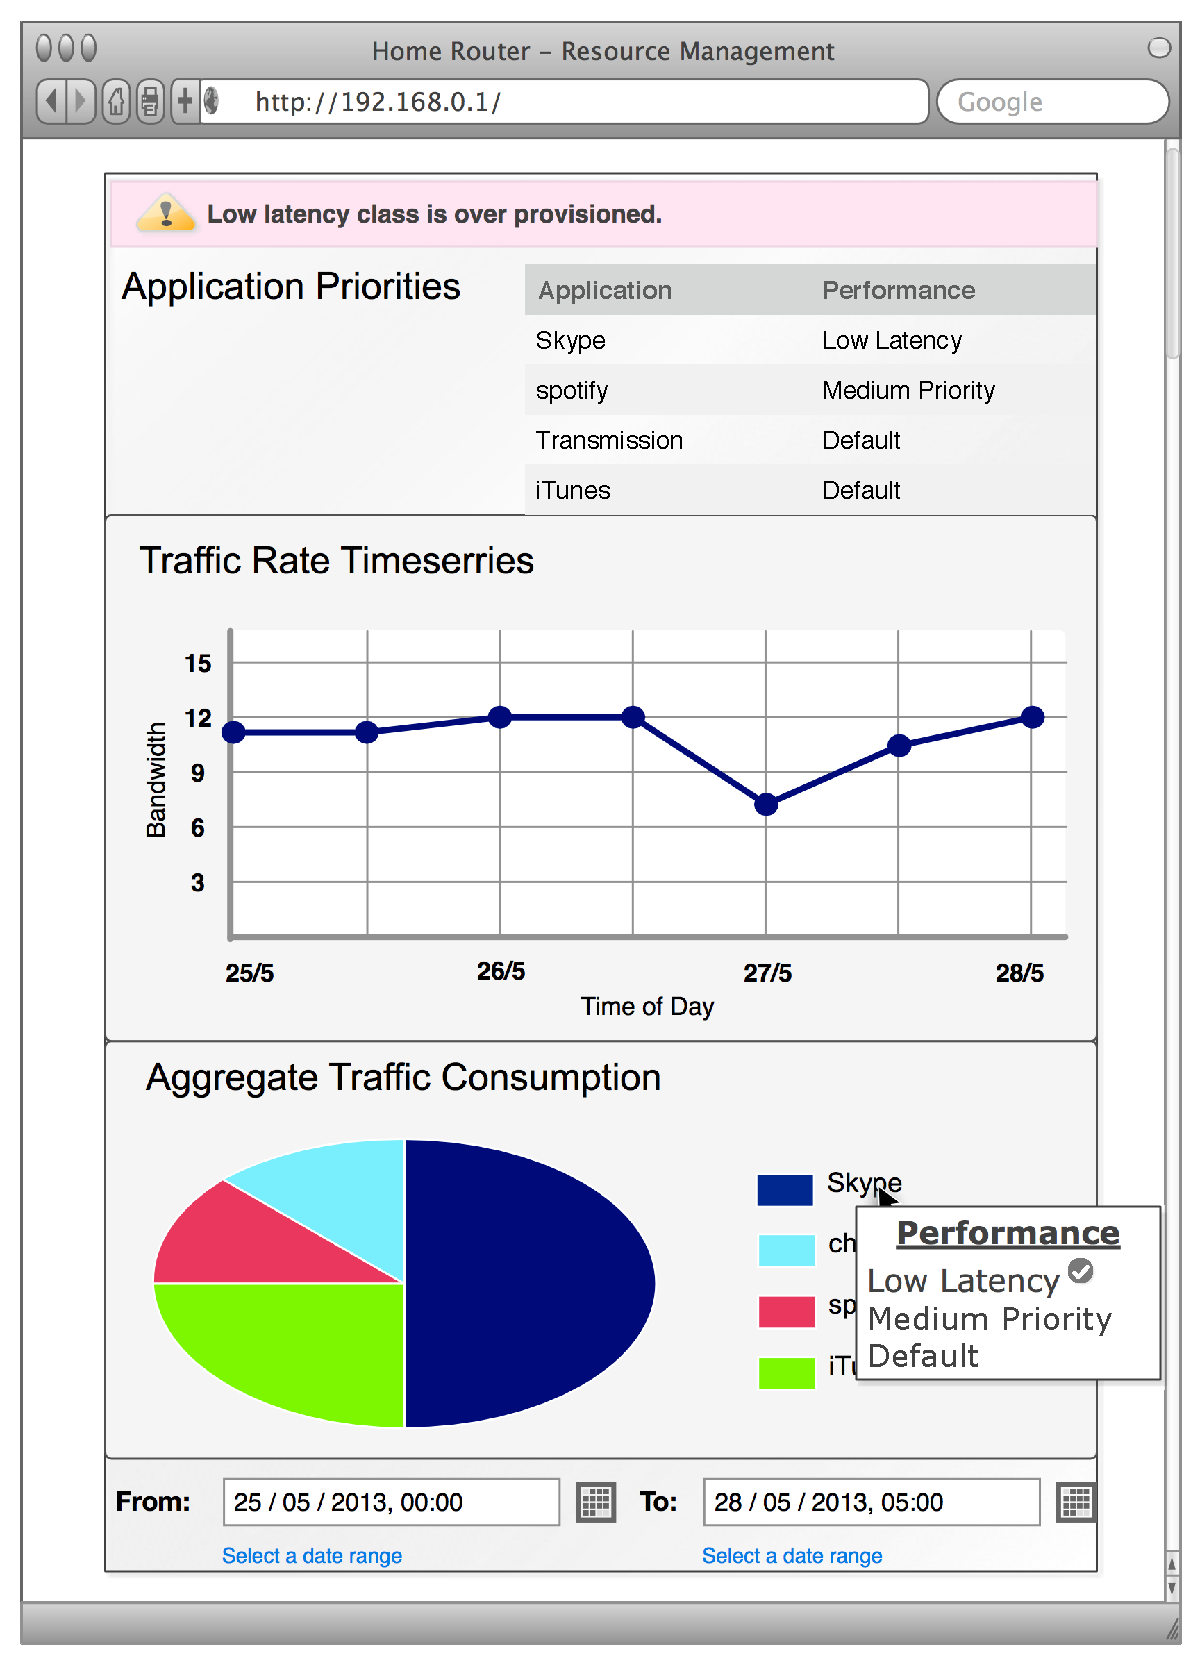
\includegraphics[width=0.8\columnwidth]{homework_intf_qos}
  \caption[QoS user interface]{\label{fig:homework_intf_qos} QoS user interface.
    The user is able to view the network utilisation per application, as well as
    express application prioritisation.}
\end{figure}

In our design, the home router is the rendez-vous point between the policies of the two
entities. In the home setting, the router is responsible to store
traffic statistics, record the user application priority, and at run-time map
application flows to the appropriate queue.  We use three tables in HWDB to
store relevant information; namely \texttt{Application tuple},
\texttt{Application timeseries} and \texttt{Application priority} tables.  The
\texttt{Application tuple} table stores mappings between applications and flow
tuples populated with data from the end-host data-collection daemons.  The
\texttt{Application timeserries} table stores per-application network
utilization information populated with data from the router using \of
\texttt{flow\_stats} message.  Finally, the \texttt{Application priority} table
stores the user's application prioritisation policy. 

We expose resource control of our system to home members through a web interface,
presented in Figure~\ref{fig:homework_intf_qos}.  Through this interface the
user can inspect per-application, aggregate and timeserries resource consumption,
retrieved from the \texttt{Application timeseries} table, and configure
application prioritisation stored in the \texttt{Application priority}.
Additionally, the interface notifies the user when the policy over-utilizes the
LLHP queue.  Specifically, we use the packet loss counter of the \of~{\tt
  queue\_stats} message to trigger notifications during high packet loss
incidents.  Through this interface, we try to address the issues raised
by~\mycite{Chetty10}. 

During operation, the proposed design extends the forwarding logic described
earlier. Specifically, for each network flow destined to a non-local host, once
the controller verifies policy compatibility, it maps the flow to an
application, using the \texttt{Application tuple} table data,  and to a priority
queue, using the \texttt{Application priority} table. The controller sends a
{\tt flow\_mod} message with an {\tt enqueue} action to assign the flow to the
appropriate queue. In addition, if the application priority is not the default,
then the controller will also send a {\tt flow\_mod} packet to the FlowVisor
instance to setup the incoming direction of the flow. 

\subsection{Evaluation} \label{s:qos:eval}

\begin{figure}
  \centering
  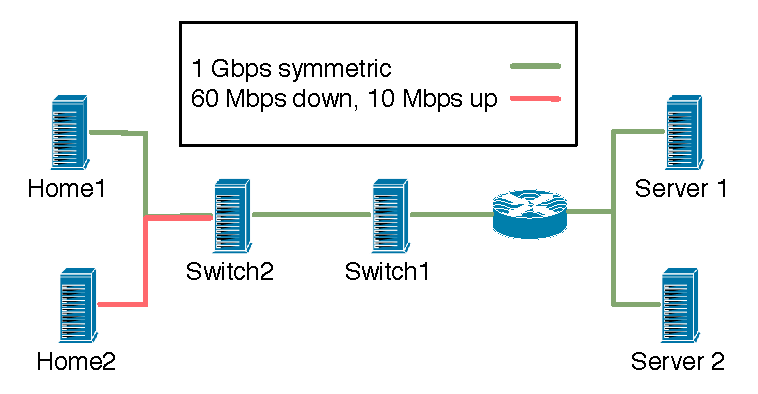
\includegraphics[width=0.6\columnwidth]{queue_eval_setup}
  \caption{\label{fig:queue_eval_setup} QoS mechanism evaluation topology.}
\end{figure}

\begin{table}
  \begin{tabular} {|l|c|l|c|}
    \hline
    \multicolumn{2}{c}{Web traffic} & Gaming traffic & \\
    \textbf{Parameter} & \textbf{Distribution} & \textbf{Parameter} & \textbf{Distribution} \\
    \hline
    objects per page    & Pareto(2.43, 3.0)       & inter-packet gap & lognormal(79.34, 0.25)\\
    inter-request delay & Pareto(1.5, 0.75)       & packet size      & Constant(0.05) \\
    inter-object delay  & Weinbull(1.46, 0.382)   & &                 \\
    object size         & lognormal(1.318, 9.357) & &   \\
    \hline
  \end{tabular} 
  \caption{\label{t:homework:performance-web-model}Model parameters for HTTP~\mycite{Barford1998} and
    gaming~\mycite{Lang2004} traffic generation.}
\end{table}


In this section, we evaluate the impact of our architecture on
performance-sensitive applications.  Figure~\ref{fig:queue_eval_setup} presents
the topology we employ for our evaluation.  \textit{Home1} and \textit{Home2}
emulate household Internet traffic,  \textit{Server1} and \textit{Server2}
emulate Internet services,  \textit{Switch1} emulates the last-mile of the ISP
network and \textit{Switch2} emulates the Internet path between the aggregation
layer of the ISP and the Internet services. In detail, Home1 emulates a single
household running a resource critical application towards Server1, while Home2
emulates an ensemble of nine households generating bursty HTTP requests towards a
web service on Server2, using the web model in
Table~\ref{t:homework:performance-web-model}.  Switch1 provides asymmetric
Internet links with 4 Mbps downlink capacity and  512 Kbps uplink capacity to
each household and  connects them to the ISP distribution network through a 4
Mbps symmetric link, thus providing a downstream subscription ratio $1:10$.
Switch2 propagates traffic between Switch1, Server1 and Server2, adding 10~msec
of one-way latency to each direction. Each node in the  topology runs on a
different host equipped with a quad core Intel CPU (Core 2 Quad Q6600), 4 Gbytes
RAM and a quad-port 1 GbE Intel card. Switch1 and Switch2 use \ovs to implement
fast packet forwarding functionality.

Using the aforementioned topology, we evaluate the impact of our architecture
on two popular applications, VoIP and Gaming. Without loss of generality, the
selected applications provide a representative set in terms of  latency and
throughput requirements.  We emulate VoIP traffic, using a constant rate 250
Kbps TCP
flow~\footnote{\url{https://support.skype.com/en/faq/FA1417/how-much-bandwidth-does-skype-need}},
while for gaming traffic we use a UDP probe based on the model presented in
Table~\ref{t:homework:performance-web-model}. We conduct the measurement for
300 seconds, initializing the network without any traffic prioritisation, and
we enable our architecture after 150 seconds of execution, assigning the HTTP
application on the default queue and the VoIP and Gaming applications on the
LLHP queue. Figures~\ref{f:homework:performance-qos-gaming}
and~\ref{f:homework:performance-qos-voip} present the results of the experiment
for the gaming and VoIP applications respectively. More specifically, we
present the per-packet latency for gaming and the instantaneous
application-perceived throughput for VoIP, along with the instantaneous
aggregate throughput of all HTTP flows. For the gaming application, we observe
that packets face significant latencies (200-500 msec), primarily due to
queueing delays when they coexisting in a congested link with HTTP flows and
the network is not using any short-term resource control. The latency is
effectively minimized when we enable our architecture without significant
performance limitation for HTTP traffic. Similarly, VoIP traffic experiences
significant throughput variations (200-350 Kbps) which are eliminated when the
flow is assigned to the LLHP queue.  The results verify that the proposed
short-term resource control mechanism can significantly improve user
experience and effectively improve network performance for applications
with strict resource requirements, while introducing minimal impact on
co-existing application performance. 

\begin{figure*} \centering
 \subfigure[Gaming]{\includegraphics[width=0.49\columnwidth]{Chapter2/Chapter2Figs/homenet-prio-gaming}\label{f:homework:performance-qos-gaming}}
 \subfigure[VoIP]{\includegraphics[width=0.49\columnwidth]{Chapter2/Chapter2Figs/homenet-prio-voip}\label{f:homework:performance-qos-voip}}
 \caption[QoS mechanism Latency and throughput evaluation]{\label{f:homework:performance-qos} Latency and throughput performance
  of the QoS architecture. The QoS mechanism is enabled after 150 seconds of
  execution, reducing significantly packet latency and providing accurate
  throughput bounds.}
\end{figure*}

\section{Summary} \label{s:conclusion}

This chapter has drawn upon previous user studies to reflect on the distinct
nature of home networks and the implications for domestic network
infrastructures.  Three particular user needs that arose from home network user
studies were for richer visibility into and greater control over the home
wireless network, as well as the home as part of the everyday management of the
home by inhabitants.  We  considered how to exploit the nature of the home
network in order to shape how it is presented and opened to user control and ultimately
to provide scalable management through a novel control plane architecture.  

We used the \ovs and NOX platforms to provide flow-based management of the home
network.  As part of this flow-based management, we exploited the social
conventions in the home to manage introduction of devices  to the network, and
their subsequent access to each other and Internet hosted services.  This
required modification of three standard protocols, DHCP, EAPOL and DNS, albeit
in their behaviour but \emph{not} their wire formats, due to the need to retain
compatibility with legacy deployed stacks. In addition, in our exploration we
presented a simple mechanism enabling home user to guide the ISP resource
allocation mechanism in order to fulfil application requirements.  Our
exploration, on one hand, provides strong evidence that appropriate design of
the control plane architecture can transform and scale the management effort,
while on the other hand, it suggests that existing presumptions could usefully
be re-examined to see if they still apply in a network context.  In the next
chapter we explore application of SDN technologies in connectivity scalability. 

% \section{Technological and Social aspects of home networking} \label{s:elephant}
% 
% The growth in the number of IP-enabled devices over the last decade  has
% expanded the use-cases for in-home wired and wireless networking; from Internet
% connection sharing to local media sharing, gaming, and other applications.  Home
% network functionality, unlike other network environments, contains a strong
% social aspect, which establishes a dynamic relationship between the technology
% and the social organisation of the setting, exhibiting some unique properties.
% In this Section, we summarize finding of relevant studies and elaborate on the
% characteristics of home network environments, both from a social and an
% engineering perspective.  More specifically, in Section~\ref{s:home_measurement}
% we present the distinct technical characteristics of home network technologies,
% while in Section~\ref{s:home_social} we focus on the social characteristics of
% home networking, using findings from relevant ethnographic studies. 
% 
% \subsection{Home Networking as a system} \label{s:home_measurement}
% 
% Home networks are highly heterogeneous edge networks, typically
% Internet-connected via a single broadband link, where non-expert network
% operators provide a wide range of services to a small set of users.
% While we focus on home networks, we note that many environments, e.g.,~small
% offices, coffee shops, hotels, exhibit similar characteristics and thus may
% benefit from similar approaches. Such capabilities are likely to be infeasible
% in more traditional settings, e.g.,~backbone and enterprise networks.  In this
% section we use existing studies to present the technical characteristics of
% modern home network. 
% % More specifically, we present the type of devices
% % connected to a home network, the properties of the local and Internet traffic
% % and the properties of local and Internet connectivity. 
% 
% % Home network measurement studies have focused both on the local network
% % properties as well as the nature of the Internet traffic. Local network analysis
% % provides useful insight on the way devices interact within the house and the
% % possible performance limitations. Such measurement studies focused mainly on
% % developing active or passive measurement tools, that runs on end-hosts in the
% % network and collect data. 
% Home networks commonly provide local device connectivity through wired and
% wireless Ethernet, both supported by modern PCs. Wired network adapters
% predominantly support the 802.3ab (1 Gbps full-duplex) standard and wireless
% network adapters support predominantly 802.11a/g (54 Mbps) standards, while
% 802.11n (600 Mbps) support is slowly increasing.  Wired Ethernet connectivity
% provides high data rates with negligible medium interferences, but fails in
% supporting flexible spatial mobility within the household. In contrast, wireless
% Ethernet connectivity supports extensive device mobility, but network
% performance is susceptible to environmental parameters.  \mycite{homenetProfiler}
% study the availability of wireless connectivity in home networks and report on
% average good signal coverage~($<$ -80dBm), verifying a significant technological
% improvement which overcomes connectivity problem highlighted by earlier
% studies~\mycite{Yarvis05characterizationof}. In addition, the authors observe
% significant wireless network overhearing,  with end-hosts  picking up 10
% wireless networks on average, a third of which used overlapping channels.  The
% accessibility of wireless networks beyond the physical home  limits highlights a
% significant access control problem. The WPA encryption scheme, used
% predominantly to mitigate this problem, ensures network data integrity but lucks
% flexibility; pre-shared key knowledge provides full access to the home network.
% 
% Home networks use predominantly ADSL and cable technologies to provide Internet
% connectivity, while fiber, 3G and satellite technologies are not uncommon. As a
% result, Internet connectivity exhibits high variance in performance, depending
% extensively on the medium and the ISP\@.  \mycite{Dischinger2007} present an early
% broadband performance study, reporting significant performance variance and a
% bottleneck on the last mile of the link.  \mycite{Sundaresan2011} contact a
% similar studies, running though measurements probes on the home router, and
% detect significant effects on network throughput and latency by ISP throttling
% mechanisms, like PowerBoost~\mycite{powerboost}. Finally, \mycite{Kreibich10} verify
% the bufferbloat problem in residential broadband ISPs.  The importance of
% Internet performance for residential broadband networks is reflected on a
% governmental level, where independent state authorities evaluate ISP service
% quality~\mycite{fcc, ofcom}.  
% 
% Home networks exhibit unique applications and traffic characteristics.
% \mycite{Reggani12} contact an in-network passive measurement and study the host
% network behaviour, under different network environments. The study concludes
% that in the home network end-hosts exhibits a distinct network behaviour,
% generating high volumes of filesystem and P2P applications, while a significant
% portion of the traffic remains local.  Residential broadband Internet traffic
% patterns exhibit significant temporal and spatial variability.  \mycite{Cho2006}
% detect in 2005 significant volumes of P2P traffic in Japanese bradband ISPs.
% More recently, \mycite{Maier2009} analyse traffic traces from a German ADSL
% provider and detect a significant shift towards web applications.
% \mycite{Erman2011} detect similar trends in US broadband traces, identifying more
% that 70\% of the network traffic being HTTP and serving primarily online video
% and one-click hosting services. 
% 
% In terms of device demographics, relevant studies identify an increase in the
% number and heterogeneity of connected devices. \mycite{homenetProfiler} present a
% user survey reporting that home networks host on average 7-8 devices. In
% addition, the users report wide variability in connected devices
% (e.g.~smartphones, tablets, game consoles, etc.), highlighting a strong openness
% requirement in any modification in the network functionality.  Nonetheless,
% \mycite{Hatonen10} test off-the-self home routers and unveil high variability in
% the semantics of the NAT and DNS implementations.  Since such routers are widely
% deployed in home networks, applications remain robust towards this variability.
% % to consider this variability as acceptable. 
% % widespread usage of such routing kit, the impact to home networking appears to be
% % minimal and home network environment appears to be resilient to non-standard
% % router implementations. 
% 
% \subsection{Home Network as a social activity} \label{s:home_social}
% 
% Home networks technologies provide an excellent setting to study the
% interactions of social behaviours and technology.  Studies in the field usually
% engage in user interviews in order to understand how users perceive and interact
% with network technologies. 
% 
% An important aspect in analysing the home network from a social aspect, requires
% an in-depth understanding of the user perception of  home network technologies.
% \mycite{shehanpoole08,grinter05} analyse user sketches presenting their network
% technology understanding and highlight two important observations; user opacity
% to the network increases inversely proportional to their user network experience
% -- verifying the effectiveness of the network abstraction, and users identify
% network devices using the social context of the home network.  Further,
% \mycite{tolmie07} perform an empirical analysis of the home member interactions
% with network technologies. Their finding point out that users appear reluctant
% to optimize network configuration, while they experience tolerable performance.
% Such tasks though can become more elegant if they have small duration and
% consist of well-defined steps. Furthermore, interest conflicts, arising due to
% resource sharing, are usually solved through negotiation between household
% members. Furthermore, relevant studies have highlighted the importance of
% accurate information of the utilization and state of the network for network
% management. \mycite{Chetty10} analyse the effect of bandwidth utilization
% visualisation in user experience, reporting improved user understanding of
% network functionality and troubleshooting, but also raised privacy concerns. 
% 
% Home network configuration and management are influenced to a great extend by
% the design of the house and the routines of the house members.  \mycite{Rodden03}
% use the~\mycite{Brand94} model of home architecture temporal evolution, to analyse
% the relationship between ubiquitous technologies and home design and understand
% the interactions between home design and network usage. The study reports that
% network decisions are severely affected by the design of the house, e.g.,
% location of the network router, while at the same time, users confuse the limits
% of the house with the limits of their network, e.g.~users declare wireless
% encryption as irrelevant, since it is contained within the limits of the house.
% % In~\mycite{rodden04,crabtree03} the authors monitor the real time communications
% % and information flows in a multi-member household. The study concludes that
% % communication activities have a location reference defined to the involved
% % member as well as the house planning, while activities can be synthesized as
% % sequences into higher order activities. Additionally, using these
% % observations, they propose a framework which can model such interactions. 
% In addition, \mycite{shehan07} analyse common management and configuration
% problems in home networks and draw parallels with respective design decisions in
% the network systems.  They present a weight of evidence, pointing out that
% problems with current network technologies are not amenable to solution via a
% `thin veneer' of user interface technology layered atop the existing
% architecture.  Rather, they are \emph{structural}, emerging from the mismatch
% between the stable `end-to-end' nature of the Internet and the highly dynamic
% and evolving nature of domestic environments.  

\chapter{Scalable User-centric cloud networking}
\ifpdf
    \graphicspath{{Chapter3/Chapter3Figs/PNG/}{Chapter3/Chapter3Figs/PDF/}{Chapter3/Chapter3Figs/}}
\else
    \graphicspath{{Chapter3/Chapter3Figs/EPS/}{Chapter3/Chapter3Figs/}}
\fi

In this chapter we explore application of the SDN technology in personal cloud
computing applications. In the recent years, the development in cloud computing
applications provided a number of popular Internet-wide services that allow
users to interconnect at the application layer and share information. Through
this approach users bypass the restrictions imposed in the Internet by deployed
middleboxes, at the cost though of exposing their information to third party
cloud service providers and reduced performance and efficiency. 

Using SDN technologies, we design an architecture that allows users to
interconnect their devices with minimum interactions with the cloud
infrastructure.The propose architecture deploy an openflow-enabled bridge and a
local controller on each device. Each controller by default forwards packets as
normal on the local network. The forwarding logic, though,  is augmenting
through a distributed coordination protocol which permits nodes to negotiate
possible connection opportunities and establish ad-hoc tunnels, enabling as a
result an Internet-wide distributed control mechanism. At the core of
our design, we tranform the naming service host abstraction. Each device
acquires a global domain name, while each name resolution triggers a connection
engine, that tries to find the best possible bidirectional channel between the
two nodes. The naming service uses the established
DNSSEC extension, providing a fully authenticated and secure control
mechanism among \signpost and applications. Further, the distributed nature
of the naming hierarchy in the Internet permits seamless control distribution.

In order to understand the impact of the proposed architecture we develop a
strawman implementation, named {\it Signpost}. Signpost implements the core of
the control logic of the proposed architecture. Additionally, it integrades a
number of network tactics of established tunneling and notification mechanisms.
Currently \signpost provides integration of the main architecture with SSH, OpenVPN,
TOR, Privoxy, Multicast-DNS and Nat punching. 

In the chapter we present in Section~\ref{sec:signpost-introduction} the
motivation for this work, followed then by the key observations for our design
in section~\ref{sec:signpost-design}. Following the results of our
observations, we present in section~\ref{sec:signpost-architecture} the
architecture of our proposed proposed strawman implementation of the controller
and the details of the tactics. Finally, in Section~\ref{sec:signpost-evaluation}
we present a number of micro-benchmark tests for our system and conclude in
Section\ref{sec:signpost-conclusion}.

\section{Introduction}\label{sec:signpost-introduction}

Present the gap in network understanding between the clients and the ISP and
present a tool that allows to bridge it.

\section{Enabling edge user-driven connectivity}\label{sec:signpost-design}

\section{Signpost Architecture}\label{sec:signpost-architecture}

\section{Evaluation}\label{sec:signpost-evaluation}

\section{Conclusions}\label{sec:signpost-conclusion}
%\section{Second Section}
%\markboth{\MakeUppercase{\thechapter. My Second Chapter }}
%and here I write more ...
%
%\subsection{first subsection in the Second Section}
%... and some more ...
%
%\subsection{second subsection in the Second Section}
%... and some more ...
%
%\subsection{third subsection in the Second Section}
%... and some more ...

% ------------------------------------------------------------------------

%%% Local Variables: 
%%% mode: latex
%%% TeX-master: "../thesis"
%%% End: 

\def\baselinestretch{1}
\chapter{Conclusions and Future Work} \label{sec:conclusions}

\def\baselinestretch{1.66}

This chapter concludes the dissertation by summarising the work it described,
and noting areas in which further work is required.

\section{Summary}

This dissertation has addressed issues of control plane performance scalability
using the SDN paradigm.  Chapter~\ref{s:introduction:introduction} began by
motivating the requirement to scale the functionality of existing network
protocols and technologies in order to support the design limitation which are
highlighted by increased adoption of networks.  We argued that control plane
performance is multi-dimensional (e.g.~resource control, management,
connectivity), which have variable importance for application and depend highly
on the deployment environment. We claimed that speciailized control plane
architectures can mitigate network bottlenecks, introduced by protocol design,
while ensuring backwards compatibility and high performance, by addressing the
requirement and opportunities of the deployed environment. 

Chapter~\ref{ch:background} then considered background and related work to the
problem of network control. We provided a bottom-up design discussion on
available network control mechanisms. We elaborated on the architecture of
current network devices and presented a generic design model of the integration
between the control and data plane in a single device in order to highlight the
physical limitations in  network performance. Furthermore, we reviewed
the current production-level network control protocols and mechanisms for the
data link and network layers and it was argued that their ability for responsive
flexible and user friendly control is reduced. Furthermore, we surveyed a
series of experimental approaches which address network control limitation and
provide flexible, distributed and evolvable control.  Namely we present Active
Network, Devolved Control of ATM Networks and Software Defined Networking. In
order to highlight the opportunities provided by these mechanisms, we concluded
this chapter with an extensive presentation of novel control applications build
on top of the SDN paradigm. 

The bulk of the experimental contribution of this dissertation was reported in
the following three chapters. Chapter~\ref{sec:sdn_scalability} analysed the
elementary scalability of the SDN paradigm. In this chapter, we presented two
measurement platforms, enabling network experimenters to evaluate the
performance of SDN architectures. \oflops is a high-precision
hardware-accelerated \of switch measurement platform which enables experimenters
to understand the performance behaviour of \of-enabled devices, and \sdnsim, a
lightweight high-precision network simulation and emulation framework. Using
\oflops, we develop and run a series of tests characterising the elementary
functionalities of the \of protocol and detect significant variance between
switch protocol implementations. \sdnsim is a high precision experimentation
environment, which allows users to implement their control logic and traffic
models and evaluate the performance of an SDN architecture. The platform
provides the ability to simulate, using the \ns{3} platform, or emulate, using
the Xen virtualisation platform, a experimental definition.  The platform
provides enhanced realism on the performance characteristics of the network
control plane, while through our evaluation we highlighted the scalability of
experimentation.  Using \sdnsim, we replicate the functionality of a small-scale
datacenter network and highlighted the effectiveness of control centralisation.

Chapter~\ref{sec:homework} elaborated the problem of management scalability in
modern home networks. Using ethnographic and measurement studies of the home
setting, we identified significant mismatches between the user-requirement and
user-understanding of network functionality and the existing technologies.
Motivated by this observation, we redesign the home router, implementing a
series of control modifications which enhance user control and bridge the user
perception with the underlying network functionality. The proposed architecture
is extended with a collaborative resource control mechanism which integrates
users application-level requirements with the ISP policy, in an effort to
develop a user-friendly control scheme for the last-mile bottleneck in
residential broadband networks. We presented the development of a strawman
implementation of our system and verified that the architectures incurs minimal
impact on network functionality, the protocol modifications remain
backwards compatible with a number of popular devices, OSes and applications and
that the resource control mechanism improves the support for latency and
bandwidth sensitive applications in congested residential networks. 

Chapter~\ref{sec:signpost} discussed Internet-scale naming and connectivity
scalability.  Through the work of this chapter, we aimed to develop a
decentralised and Internet-wide federated network between the devices of a user.
We motivated our effort by presenting the limitations of existing approaches in
terms of usability and privacy and argued that an evolved control plane for
end-hosts can address such limitations and support all required functionality.
We proposed the \signpost architecture providing secure, continuous and
decentralised inter-device connectivity. \signpost reuses existing connectivity
mechanisms to provide ad-hoc end-to-end path between devices. The system
provides a global naming structure and uses the DNS protocol to establish a
global control channel through which \signpost automates distributed evaluation
and configuration of connection establishing mechanisms.  We presented a
strawman implementation  of the \signpost architecture and its integration with
the \openvpn, TOR, SSH, Privoxy, NAT punching and DNS-SD mechanisms.  Using the
\signpost strawman implementation, we characterised the low impact of the
architecture to network functionality and its backwards compatibility with
existing applications. 

\section{Summary of Contributions}

The dissertation makes the following three contributions:

\paragraph{Control plane scalability} 
In this thesis we present the first scalability characterisation of \of
implementations. We highlighted the significant performance diversity between
implementations which can affect the performance and the correctness of control
architectures.  Furthermore, we developed \sdnsim, an experimentation platform
for SDN architectures, providing the ability to emulate and simulate network
experiments. \sdnsim provides high fidelity on replicating the control channel
of the network and provides intuitive control between fidelity and scalability. 
Using \sdnsim we evaluate the performance of a hierarchical control architecture
in a small-scale datacenter.

\paragraph{Management scalability}

This thesis presented a novel control architecture establishing scalable
management for home network. We presented a flow-based controller, which exploit
the social conventions in the home to manage introduction of devices  to the
network, and their subsequent access to each other and Internet hosted services.
Additionally, we proposed a modification in the control architecture of the ISP
network, which enables users to express and enforce their resource requirements
in a user-friendly manner. We provided strong evidence on the scalability,
backwards compatibility and effectiveness of our solution.  

\paragraph{Connectivity and naming scalability}

This thesis analysed the significant limitation introduced by the current
Internet architecture on the connectivity ability between the devices of users.
In order to mitigate these limitations we presented \signpost, a decentralised
control architecture providing global names for user devices and continuous
connectivity between them. We presented the flexibility of \signpost to
encapsulate a wide range of connection establishing mechanism and provided
strong evidence on its backward-compatibility with existing applications and its
performance scalability. 

\section{Future Work}
  
The experimental results and the practical solutions presented in the thesis
provide fruitful seeds to cultivate a wider research agenda on control plane
evolvability.

\subsection{Distributed network control}

One the first use cases of the SDN paradigm was the centralisation of control in
order to improve policy effectiveness and ease network management.  Nonetheless this
vision has evolved and refocuses on the development of distributed control
architectures. Control distribution is motivated by two observations.  Firstly,
load and latency of the control channel increases proportionally to the size of the
network, while reliability guarantees relax. Secondly,
defining one global control policy which is able to encapsulate multiple policy
aspects (e.g.~security, performance, access control) exhibits significant
complexity. Applications have shifted to a multi-controller paradigm using
either centralised proxies~\cite{flowvisor-osdi} or separating the network
in domains and use distribute algorithms to synchronise state between
controllers~\cite{Koponen10}. 

The work presented in Chapter~\ref{sec:sdn_scalability} provide a scalable
control experimentation platform, a powerful tool to understand further the
impact of  distributed design patterns on the performance of a network.
Hierarchical control, as presented through the evaluation experiment using the
\sdnsim, has low impact on network performance, but a complete architectural
design requires further evaluation of mechanisms with strong control plane
responsiveness and reliability guarantees. 

\subsection{User-centric networking}

As we have discussed in Chapter~\ref{sec:homework}, current network technologies
exhibit a significant mismatch with the user requirements. The outcomes from the
previous two chapter have provided strong evidence on the ability of networks to
reconsider control and augment it with meaningful user input. Rather than
relegating users to an artifact of the application layer, accommodating users
and their relationships at all layers of the system can improve user
satisfaction and network functionality. We consider two main extensions on the
work of the thesis, towards this goal. 

Firstly, a number of areas arise from the work in Chapter~\ref{sec:homework}.
The presented control architecture provides novel opportunities to augment home
network functionality and exploit the wider social context of the home setting.
In the local network, home guests can inject their configuration in the local
network policy and improve their experience. This approach is not limited in
the local network and can expand to wider contexts. For example, neighbours can
negotiate  resource control by taking advantage of the social context in a
neighbourhood. Users can coordinate socially to share unutilized resources on
the last mile of the residential connection,  e.g.~exchange high priority
traffic for specific timeslots with neighbours.

Secondly, a number of pieces of work arise from Chapter~\ref{sec:signpost}.  The
\signpost design at the moment is limited in its policy expressiveness, which
though is sufficient to address our motivations.  Nonetheless, the
authentication primitives can provide a scalable and global mechanism to develop
novel network policy frameworks and address a series of problems stemming from
the inability of the network layer to authenticate network end-points.
Furthermore, the hierarchical structure of the \signpost architecture can be
used to reflect higher level social relationship and increase the in-network
flexibility. Bigraph theory provides a sufficient framework to model and scale
the complexity of such control designs. 

% For example, the devices of a user who is a member of the University
% of Cambridge can connect through the \signpost architecture with the university
% network control plane,  when a device is connected to the university network. 
% At run-time the device \signpost daemon can negotiate with the university
% \signpost controller the device network requirements and reflect them in the
% University network control.

\section{Conclusion}

In summary, this dissertation has argued that network technologies exhibit
significant limitation to scale their functionality and support the multiple
aspects of network performance. We identified these limitations on the
unforeseen functional requirements occurring  by the wide adoption of network
technologies. In order to address these limitations, we content that network
control must be redesign and specialized in order to fit the requirements and
the take advantage the properties of the deployment environment. This
dissertation has presented and evaluated mechanisms to control plane
functionality, management and connectivity scalability. 





\backmatter % book mode only
\appendix
%\include{Appendix1/appendix1}
%\include{Appendix2/appendix2}

\bibpunct{[}{]}{,}{a}{}{;}

\bibliographystyle{plainnat}
% \bibliographystyle{Classes/CUEDbiblio}
% \bibliography{plain}
% \bibliographystyle{Classes/jmb}
\renewcommand{\bibname}{References} % changes default name Bibliography to References
\bibliography{References/references-bk,References/rfc-bk} % References file

\end{document}
